\documentclass[11pt,]{article}
\usepackage{lmodern}
\usepackage{amssymb,amsmath}
\usepackage{ifxetex,ifluatex}
\usepackage{fixltx2e} % provides \textsubscript
\ifnum 0\ifxetex 1\fi\ifluatex 1\fi=0 % if pdftex
  \usepackage[T1]{fontenc}
  \usepackage[utf8]{inputenc}
\else % if luatex or xelatex
  \ifxetex
    \usepackage{mathspec}
  \else
    \usepackage{fontspec}
  \fi
  \defaultfontfeatures{Ligatures=TeX,Scale=MatchLowercase}
  \newcommand{\euro}{€}
\fi
% use upquote if available, for straight quotes in verbatim environments
\IfFileExists{upquote.sty}{\usepackage{upquote}}{}
% use microtype if available
\IfFileExists{microtype.sty}{%
\usepackage{microtype}
\UseMicrotypeSet[protrusion]{basicmath} % disable protrusion for tt fonts
}{}
\usepackage[margin=1in]{geometry}
\usepackage{hyperref}
\PassOptionsToPackage{usenames,dvipsnames}{color} % color is loaded by hyperref
\hypersetup{unicode=true,
            pdfborder={0 0 0},
            breaklinks=true}
\urlstyle{same}  % don't use monospace font for urls
\usepackage{color}
\usepackage{fancyvrb}
\newcommand{\VerbBar}{|}
\newcommand{\VERB}{\Verb[commandchars=\\\{\}]}
\DefineVerbatimEnvironment{Highlighting}{Verbatim}{commandchars=\\\{\}}
% Add ',fontsize=\small' for more characters per line
\usepackage{framed}
\definecolor{shadecolor}{RGB}{248,248,248}
\newenvironment{Shaded}{\begin{snugshade}}{\end{snugshade}}
\newcommand{\KeywordTok}[1]{\textcolor[rgb]{0.13,0.29,0.53}{\textbf{{#1}}}}
\newcommand{\DataTypeTok}[1]{\textcolor[rgb]{0.13,0.29,0.53}{{#1}}}
\newcommand{\DecValTok}[1]{\textcolor[rgb]{0.00,0.00,0.81}{{#1}}}
\newcommand{\BaseNTok}[1]{\textcolor[rgb]{0.00,0.00,0.81}{{#1}}}
\newcommand{\FloatTok}[1]{\textcolor[rgb]{0.00,0.00,0.81}{{#1}}}
\newcommand{\ConstantTok}[1]{\textcolor[rgb]{0.00,0.00,0.00}{{#1}}}
\newcommand{\CharTok}[1]{\textcolor[rgb]{0.31,0.60,0.02}{{#1}}}
\newcommand{\SpecialCharTok}[1]{\textcolor[rgb]{0.00,0.00,0.00}{{#1}}}
\newcommand{\StringTok}[1]{\textcolor[rgb]{0.31,0.60,0.02}{{#1}}}
\newcommand{\VerbatimStringTok}[1]{\textcolor[rgb]{0.31,0.60,0.02}{{#1}}}
\newcommand{\SpecialStringTok}[1]{\textcolor[rgb]{0.31,0.60,0.02}{{#1}}}
\newcommand{\ImportTok}[1]{{#1}}
\newcommand{\CommentTok}[1]{\textcolor[rgb]{0.56,0.35,0.01}{\textit{{#1}}}}
\newcommand{\DocumentationTok}[1]{\textcolor[rgb]{0.56,0.35,0.01}{\textbf{\textit{{#1}}}}}
\newcommand{\AnnotationTok}[1]{\textcolor[rgb]{0.56,0.35,0.01}{\textbf{\textit{{#1}}}}}
\newcommand{\CommentVarTok}[1]{\textcolor[rgb]{0.56,0.35,0.01}{\textbf{\textit{{#1}}}}}
\newcommand{\OtherTok}[1]{\textcolor[rgb]{0.56,0.35,0.01}{{#1}}}
\newcommand{\FunctionTok}[1]{\textcolor[rgb]{0.00,0.00,0.00}{{#1}}}
\newcommand{\VariableTok}[1]{\textcolor[rgb]{0.00,0.00,0.00}{{#1}}}
\newcommand{\ControlFlowTok}[1]{\textcolor[rgb]{0.13,0.29,0.53}{\textbf{{#1}}}}
\newcommand{\OperatorTok}[1]{\textcolor[rgb]{0.81,0.36,0.00}{\textbf{{#1}}}}
\newcommand{\BuiltInTok}[1]{{#1}}
\newcommand{\ExtensionTok}[1]{{#1}}
\newcommand{\PreprocessorTok}[1]{\textcolor[rgb]{0.56,0.35,0.01}{\textit{{#1}}}}
\newcommand{\AttributeTok}[1]{\textcolor[rgb]{0.77,0.63,0.00}{{#1}}}
\newcommand{\RegionMarkerTok}[1]{{#1}}
\newcommand{\InformationTok}[1]{\textcolor[rgb]{0.56,0.35,0.01}{\textbf{\textit{{#1}}}}}
\newcommand{\WarningTok}[1]{\textcolor[rgb]{0.56,0.35,0.01}{\textbf{\textit{{#1}}}}}
\newcommand{\AlertTok}[1]{\textcolor[rgb]{0.94,0.16,0.16}{{#1}}}
\newcommand{\ErrorTok}[1]{\textcolor[rgb]{0.64,0.00,0.00}{\textbf{{#1}}}}
\newcommand{\NormalTok}[1]{{#1}}
\usepackage{graphicx,grffile}
\makeatletter
\def\maxwidth{\ifdim\Gin@nat@width>\linewidth\linewidth\else\Gin@nat@width\fi}
\def\maxheight{\ifdim\Gin@nat@height>\textheight\textheight\else\Gin@nat@height\fi}
\makeatother
% Scale images if necessary, so that they will not overflow the page
% margins by default, and it is still possible to overwrite the defaults
% using explicit options in \includegraphics[width, height, ...]{}
\setkeys{Gin}{width=\maxwidth,height=\maxheight,keepaspectratio}
\setlength{\parindent}{0pt}
\setlength{\parskip}{6pt plus 2pt minus 1pt}
\setlength{\emergencystretch}{3em}  % prevent overfull lines
\providecommand{\tightlist}{%
  \setlength{\itemsep}{0pt}\setlength{\parskip}{0pt}}
\setcounter{secnumdepth}{5}

%%% Use protect on footnotes to avoid problems with footnotes in titles
\let\rmarkdownfootnote\footnote%
\def\footnote{\protect\rmarkdownfootnote}

%%% Change title format to be more compact
\usepackage{titling}

% Create subtitle command for use in maketitle
\newcommand{\subtitle}[1]{
  \posttitle{
    \begin{center}\large#1\end{center}
    }
}

\setlength{\droptitle}{-2em}
  \title{\LARGE{SAA and SAMC for minimum graph bisection} \vspace{1pc}}
  \pretitle{\vspace{\droptitle}\centering\huge}
  \posttitle{\par}
  \author{\Large{Tyler Grimes} \vspace{1pc}}
  \preauthor{\centering\large\emph}
  \postauthor{\par}
  \predate{\centering\large\emph}
  \postdate{\par}
  \date{\today}


% Redefines (sub)paragraphs to behave more like sections
\ifx\paragraph\undefined\else
\let\oldparagraph\paragraph
\renewcommand{\paragraph}[1]{\oldparagraph{#1}\mbox{}}
\fi
\ifx\subparagraph\undefined\else
\let\oldsubparagraph\subparagraph
\renewcommand{\subparagraph}[1]{\oldsubparagraph{#1}\mbox{}}
\fi

\usepackage{times}
\usepackage{amsmath, amsthm, amssymb}
%\usepackage{hanging} %For hanging indent in bibliography.
\usepackage{enumerate} %For numbered lists.
\usepackage{enumitem} %To change subitem numbering (1.1), (1.2), etc
\setlist[enumerate]{labelsep=*, leftmargin=1.5pc, noitemsep}
\setlist[enumerate, 1]{label=(\arabic*)}
\setlist[enumerate, 2]{label=(\arabic{enumi}.\arabic*), leftmargin=2.2pc}
\setlist[enumerate, 3]{label=(\arabic{enumi}.\arabic{enumii}.\arabic*), leftmargin=3pc}
%\setlist[enumerate]{label*=\arabic*.}
\usepackage{geometry}
 \geometry{
 lmargin = 1.5in,
 rmargin = 1.5in,
 tmargin = 1in,
 bmargin = 1in
 }
\allowdisplaybreaks

\begin{document}
\maketitle

\setlength{\parindent}{2em} \setlength{\parskip}{0em}

\section{Introduction}\label{introduction}

Let \(G = (V, E)\) be an undirected graph with verticies
\(V = \{1, ..., n\}\) having weights \(w_i\) with \(0<w_i\leq p\) for
\(i = 1,...,n\) and some positive constant \(p\), and \(m = |E|\) edges
with weights \(c_{i, j} \geq 0\) for \(i, j = 1, ...,n\) where
\(c_{i, j} = 0\) indicates that there is no edge between verticies \(i\)
and \(j\).

There are many variations to the graph partition problem. In general,
consider the problem of partitioning the verticies into \(k\) disjoint
\emph{admissible} sets, \(A_1, ..., A_k\), with
\(V = A_1 \cup ... \cup A_k\). A vertex set \(A\) is admissible if
\(size(A) = \sum_{j \in A}w_j \leq p\). A partition is admissible if
each set in the partition is admissible.

A partition generates a graph cut after removing all edges between
verticies in different subsets. That is, for each \(i \in V\), set
\(c_{i, j} = 0\) if \(i\) and \(j\) are not in the same subset. For a
given partition \(A_1, ..., A_k\), we can denote the set of removed
edges by
\(R_{A_1, ..., A_k} = \left\{\{i, j\}: \{i, j\} \not\subset A_p \ \text{for any} \ p\right\} \subseteq E\),
or similarly, the set of retained edges
\(K_{A_1, ..., A_k} = \left\{\{i, j\}: \{i, j\} \subset A_p \ \text{for some} \ p\right\} \subseteq E\).
The \emph{external cost} of a partition is defined as
\(E(A_1, ..., A_k) = \sum_{\{i, j\} \in R} c_{i, j}\), that is, the sum
of all removed edge weights. The \emph{internal cost} of a partition is
defined as \(I(A_1, ..., A_k) = \sum_{\{i, j\} \in K} c_{i, j}\), that
is, the sum of all retained edge weights.

The optimization problem is to find an admissible partition that has
minimal external cost. Note that the solution to this problem need not
be unique. In addition, since the total weight of all edges is constant,
this problem is equivalent to finding an admissible partition that has
maximal internal cost.

\subsection{Brute force search and computational
complexity}\label{brute-force-search-and-computational-complexity}

An exact solution can be found by a brute force search. This procedure
would entail iterating through all possible partitions and calculating
the external cost of each. If an admissible partition is found that has
the lowest cost observed up to that point, the solution is updated to be
this partition. This method is simple, but is intractible even for small
graphs. Consider the graph of \(n\) verticies with all verticies having
weight \(w_i = 1\), and we wish to find a partition of \(k\) subsets
each of size \(p\) where \(kp = n\). There are
\(\left(\begin{matrix} n \\ p \end{matrix}\right)\) ways to choose the
first subset, \(\left(\begin{matrix} n - p \\ p \end{matrix}\right)\)
ways to choose the second, and so on. We don't care about the \(k!\)
ways of ording the subsets, so the total number of partitions is \[
\frac{1}{k!}\left(\begin{matrix} n \\ p \end{matrix}\right)
\left(\begin{matrix} n-p \\ p \end{matrix}\right)
...
\left(\begin{matrix} 2p \\ p \end{matrix}\right)
\left(\begin{matrix} p \\ p \end{matrix}\right).
\] With just 30 verticies and \(k=2\) partitions (\(p = 15\)), there are
on the order of 10\^{}7 partitions. With 100 verticies, that number
grows to over 10\^{}28. It turns out that this problem is NP-complete
(Gary \& Johnson, 1979), and so an efficient approximation method is
desirable.

\subsection{Heuristics}\label{heuristics}

Instead of using a method that guaruntees to find the global optimum,
heuristic techniques are employed which run faster and provide good, but
not always optimal, solutions. One class of heuristics iteratively
improves a partition by swapping or moving verticies between partitions
one at a time. This class is referred to as move-based algorithms or
local searches. One such method is the Kernighan-Lin (KL) algorithm
(Kernighan \& Lin, 1970). However, these approaches can get stuck at a
local optimum. This leads to the second class of heuristics, namely,
stochastic methods, which can avoid local trips. An early application of
simmulated annealing was used in this context (Kirkpatrick, 1984).

To handle very large graphs, multilevel approaches have been proposed
(Karypis \& Kumar, 1995). However, these methods still rely on local
search and stochastic methods to refine their solutions.

The remaining sections provide a brief summary of the KL and simulated
annealing algorithms, followed by two proposed heuristics based on SAA
and SAMC. Our attention will be restricted to the minimum graph
bisection problem (that is, where \(k=2\) and \(kn = p\)). A small
simulation is run for a cursory investigation into the performance of
these four methods.

\section{Kernighan-Lin (KL) algorithm}\label{kernighan-lin-kl-algorithm}

The KL algorithm (Kernighan \& Lin, 1970) is a heuristic that runs in
\(O(n^3)\) time. The procedure starts with a random partition. It then
iteratively finds a pair of verticies in each subset that gives the
largest decrease (or smallest increase) in cut size if the two are
swapped. This pair is then locked, and the procedure repeats until all
verticies are locked. At the end, the subset of swaps that gives the
total largest decrease in cut size is chosen, and the swaps are
performed. If none of the swaps reduce the cut size, then the initial
partition is left unchanged. The resulting partition can then be fed
back into the procedure, repeating the algorithm until the cut size can
no longer be decreased (a local optimal is found).

This algorithm can be extended to handle \(k\)-way partitions, unequal
size partitions, and unequally weighted verticies, however the addition
of dummy verticies is required for the latter two.

\vspace{2pc}\hrule

\vspace{0.2cm}

\noindent\textbf{KL algorithm}:

\vspace{-0.5cm}\begin{flalign*}
\textit{Parameters}\text{:} \  &\text{$W$ - a $2n \times 2n$ adjacency matrix.} &\\ 
&\text{$A$ - optional: start from an initial partition $A$ and $\bar{A}$. $A$ must be of length $n$.}
\end{flalign*}\vspace{-0.5cm}

\begin{enumerate}
\item If $A$ is not provided, initialize $A$ and $\bar{A}$ by randomly assigning $n$ verticies to $A$ and the rest to $\bar{A}$.
\item For each vertex $c$, initialize the external cost $E_c = \sum_{v\in\bar{C}} W_{cv}$, the internal cost $I_c = \sum_{v\in C} W_{cv}$, and the D-value (cost reduction for moving $c$) $D_c = E_c - I_c$, where $C$ is the partition subset containing $c$.
\item For i in 1 to n:
  \begin{enumerate}
  \item Compute the cost reduction $g_{aa'} = D_a + D_{a'} - 2W_{aa'}$ of each pair of unlocked verticies $a \in A$ and $a' \in \bar{A}$.
  \item Find the pair $(a, a')$ that has maximal cost reduction $g_{aa'}$.
  \item Set $(a_i, a_i') = (a, a')$, $\hat{g}_i = g_{aa'}$ and mark $a$ and $a'$ as locked.
  \item Update $D_x' = D_x + 2W_{xa} - 2W_{xa'}$ and $D_y' = D_y + 2W_{ya} - 2W_{ya'}$ for all unlocked $x \in A$ and unlocked $y \in \bar{A}$.
  \end{enumerate}
\item Find $k$ such that $G_k = \sum_{i=1}^k \hat{g}_i$ is maximized.
\item If $G_k > 0$, swap each pair $(a_i, a_i')$ for $i = 1, ..., k$.
\item Return $A$ and $\bar{A}$
\end{enumerate}\hrule

\section{Simulated annealing (SA)}\label{simulated-annealing-sa}

Simulated annealing was introduced by Kirkpatrick (1984) who also showed
how it can be applied to the graph bisection problem. Johnson et al.
(1989) reported on an extended empirical study comparing SA to KL. It
was shown that SA performed better on sparse random graphs, but worse on
graphs with geometric structure.

For the minimum graph bisection problem, a potential solution \(S\)
forms a partition \(\left\{S, \bar{S}\right\}\), with both subsets
having equal size. A neighbor \(S'\) of \(S\) is a partition obtained by
swapping one pair of verticies \((a, b)\), \(a\in S\) and
\(b \in \bar{S}\). The cost of a solution
\(cost(S) = \sum_{i \in S, j \in \bar{S}} W_{ij}\) is the external cost
of the partition.

The minimization problem is to find

\begin{equation}\label{minimization}
S = \min_{S \in \chi} cost(S),
\end{equation}

\noindent where \(\chi\) is the set of all possible bipartitions. This
minimization problem is equivalent to sampling from the Boltzmann
distribution

\begin{equation}\label{boltzmann}
P_{\tau*}(S) \propto \exp\{-cost(S)/\tau*\}
\end{equation}

\noindent as the temperature \(\tau*\) is lowered toward zero on a
logarithmic cooling schedule (Kirkpatrick et al., 1983). However, log
cooling is usually too slow be of use, so we instead approximate the
procedure by using a square-root cooling schedule.

\vspace{2pc}\hrule

\vspace{0.2cm}

\noindent\textbf{SA algorithm}:

\vspace{-0.5cm}\begin{flalign*}
\textit{Parameters}\text{:} \  &\text{$W$ - a $2n \times 2n$ adjacency matrix.} &\\
&\text{$\tau_0$ - the starting temperature (must be strictly positive).}
\end{flalign*}\vspace{-1cm}

\begin{enumerate}
\item Initialize a solution $S$ by randomly assigning $n$ verticies to $A$ and the rest to $\bar{A}$.
\item Set the initial temperature $\tau = \tau_0$.
\item While not yet frozen:
  \begin{enumerate}
    \item Pick a random neighbor $S'$.
    \item Compute $\Delta = cost(S) - cost(S')$.
    \item Set $S_{t + 1} = S'$ with probability $min(1, \exp(-\Delta/\tau))$. Else $S_{t + 1} = S_{t}$.
    \item Cool the temperature $\tau_{t + 1} = \tau_0/\sqrt{\text{t}}$.
  \end{enumerate}
\item Return the $S$ with the lowest cost.
\end{enumerate}\hrule

\vspace{2pc}

The procedure should be iterated until convergence; however, determining
whether the procedure has converged is difficult. Instead, the procedure
can be run for a fixed number of iterations, or until the temperature is
lowered below some threshold.

\section{Simulated stochastic annealing approximation
(SAA)}\label{simulated-stochastic-annealing-approximation-saa}

The SAA algorithm (Liang et al., 2014) can be applied to the graph
partitioning problem. This is a direct extention of SA, only now a
record is maintained of where we have been in the sample space. This
history is taken into account when deciding on an uphill move, making
the move more likely if the region has not been explored in a while. The
sample space is partitioned into \(m\) subsets

\begin{align*}
E_1 &= \{S : cost(S) \leq c_1\}, ..., \\
E_{m - 1} &= \{S : c_{m - 2} < cost(S) \leq c_{m-2}\}, \\
E_{m} &= \{S : cost(S) > c_{m - 1}\},
\end{align*}

\noindent where \(c_1 < ... < c_{m - 1}\) are user specified values. The
Boltzmann distribution from (\ref{boltzmann}) is adjusted to

\begin{equation}
P_{\theta_t, \tau_{t + 1}}(S) \propto \sum_{i = 1}^{m} \exp \left\{-cost(S)/\tau_{t + 1} - \theta_{t}^{(i)}\right\}I(S \in E_i),
\end{equation}

\noindent where \(I(\cdot)\) is the indicator function, \(\theta_t\) is
a vector of length \(m\) with \(\theta_1\) initialized to zero and
\(\theta_{t + 1} = \theta_t + \gamma_{t + 1}H_{\tau_{t + 1}}(\theta_t, S_{t+1})\),
\(\gamma_t = \left(\frac{T_0}{max(t, T_0)}\right)\) is the gain factor
sequence, \(\tau_t = \tau_0/\sqrt{t}\) is the temperature sequence,
\(H_{\tau_{t + 1}}(\theta, S) = e_{J(S)} - \pi\), \(e_{J(S)}\) is a
vector of \(m-1\) zeroes and a \(1\) at the \(J(S)\)'th index, \(J(S)\)
is the index of \(E\) that \(S\) is in, and
\(\pi_i = \frac{\exp(-\eta(i - 1))}{\sum_{k = 1}^{m}\exp(-\eta(i - 1))}\)
is the desired sampling distribution over the partition (\(\eta = 0.05\)
will be used).

\vspace{2pc}\hrule

\vspace{0.2cm}

\noindent\textbf{SAA algorithm}:

\vspace{-0.5cm}\begin{flalign*}
\textit{Parameters}\text{:} \  &\text{$W$ - a $2n \times 2n$ adjacency matrix.} &\\
&\text{$\tau_0$ - the starting temperature (must be strictly positive).} &\\
&\text{$E$ - the partition of the sample space.}
\end{flalign*}

\begin{enumerate}
\item Initialize a solution $S_1$ by randomly assigning $n$ verticies to $A$ and the rest to $\bar{A}$.
\item Initialize $t = 1$, $\tau_t = \tau_0$, $\theta_t = 0$
\item While not yet frozen:
  \begin{enumerate}
    \item Pick a random neighbor $S'$
    \item Compute $\Delta = cost(S) - cost(S')$.
    \item Set $S_{t + 1} = S'$ with probability $\min\left(1, \exp(-\Delta/\tau + \theta_{J(S)} - \theta_{J(S')})\right)$. Else set $S_{t+1} = S_{t}$
    \item Update $\theta_{t + 1} = \theta_t + \gamma_{t + 1}(e_{J(S_{t + 1})} - \pi))$
    \item Cool the temperature $\tau_{t + 1} = \tau_0/\sqrt{t + 1}$.
    \item Set $t = t + 1$
  \end{enumerate}
\item Return the $S$ with the lowest cost.
\end{enumerate}\hrule

\section{Stochastic approximation Monte Carlo
(SAMC)}\label{stochastic-approximation-monte-carlo-samc}

The SAMC algorithm (Liang et al., 2007) can also be applied to the graph
partitioning problem. This is a sampling procedure that partitions the
sampling space in the same way as SAA. However, there is no annealing
here. The target distribution is,

\begin{equation}
P_{\theta_t}(S) \propto \sum_{i = 1}^{m} \exp \left\{-cost(S) - \theta_{t}^{(i)}\right\}I(S \in E_i).
\end{equation}

Recall that \(\theta\) is updated by
\(\theta_{t + 1} = \theta_t + \gamma_{t + 1}(e_{J(S_{t + 1})} - \pi))\).
If \(\pi\) is uniform, then SAMC performs a random walk along the
subregions. By setting
\(\pi_i = \frac{\exp(-0.05(i - 1))}{\sum_{k = 1}^{m}\exp(-0.05(i - 1))}\),
the sampler is encouraged to spend more time in the lower subregions.
Although there is no guaruntee of converging to a global minimum, SAMC
is immune to local traps and will continuously explore the low
subregions.

\vspace{2pc}\hrule

\vspace{0.2cm}

\noindent\textbf{SAMC algorithm}:

\vspace{-0.5cm}\begin{flalign*}
\textit{Parameters}\text{:} \  &\text{$W$ - a $2n \times 2n$ adjacency matrix.} &\\
&\text{$E$ - the partition of the sample space.} &\\
&\text{$ITER$ - the number of iterations to perform.}
\end{flalign*}\vspace{-1cm}

\begin{enumerate}
\item Initialize a solution $S_1$ by randomly assigning $n$ verticies to $A$ and the rest to $\bar{A}$.
\item Initialize $t = 1$ and $\theta_t = 0$
\item For ITER iterations:
  \begin{enumerate}
    \item Pick a random neighbor $S'$
    \item Compute $\Delta = cost(S) - cost(S')$.
    \item Set $S_{t + 1} = S'$ with probability $\min\left(1, \exp(-\Delta + \theta_{J(S)} - \theta_{J(S')})\right)$. Else set $S_{t+1} = S_{t}$
    \item Update $\theta_{t + 1} = \theta_t + \gamma_{t + 1}(e_{J(S_{t + 1})} - \pi))$
    \item Set $t = t + 1$
  \end{enumerate}
\item Return the $S$ with the lowest cost.
\end{enumerate}\hrule

\vspace{2pc}

\section{Simulation}\label{simulation}

A small simulation study is performed to compare the four procedures.
The first task is to generate a graph. The structure of the graph should
be given consideration, as each method will perform differently
depending on the properties of the graph. However, we only consider
sparce graphs here, with each node being connected to 5\% of the other
nodes on average. After the edges are determined, the edge weights are
each generated independently from a uniform distribution. Graphs of size
\(n = 100, 250, 500, 750, 1000, 2000, 5000,\) and \(10000\) were
considered.

The initial temperature for the SA and SAA procedures are set at
\(\tau_0 = 100\). For SAA and SAMC, a partition size of \(m = 101\) is
used. To determine the upper and lower thresholds for the partition, the
minimum cost \(c^*\) from the first 1000 iterations of SA is used. Set
\(c_1 = 0.8c^*\) and \(c_{m - 1}=1.5c^*\). The \(T_0\) used by the gain
factor is set to \(5000\).

The KL algorithm is applied iteratively by passing back in the partition
it produces until it can no longer improve the partition. The SA, SAA,
and SAMC methods are run for \(10^5\) iterations each. The results from
one sample of each graph size are shown below.

\begin{figure}[hbpt]
  \begin{tabular}{cc}
    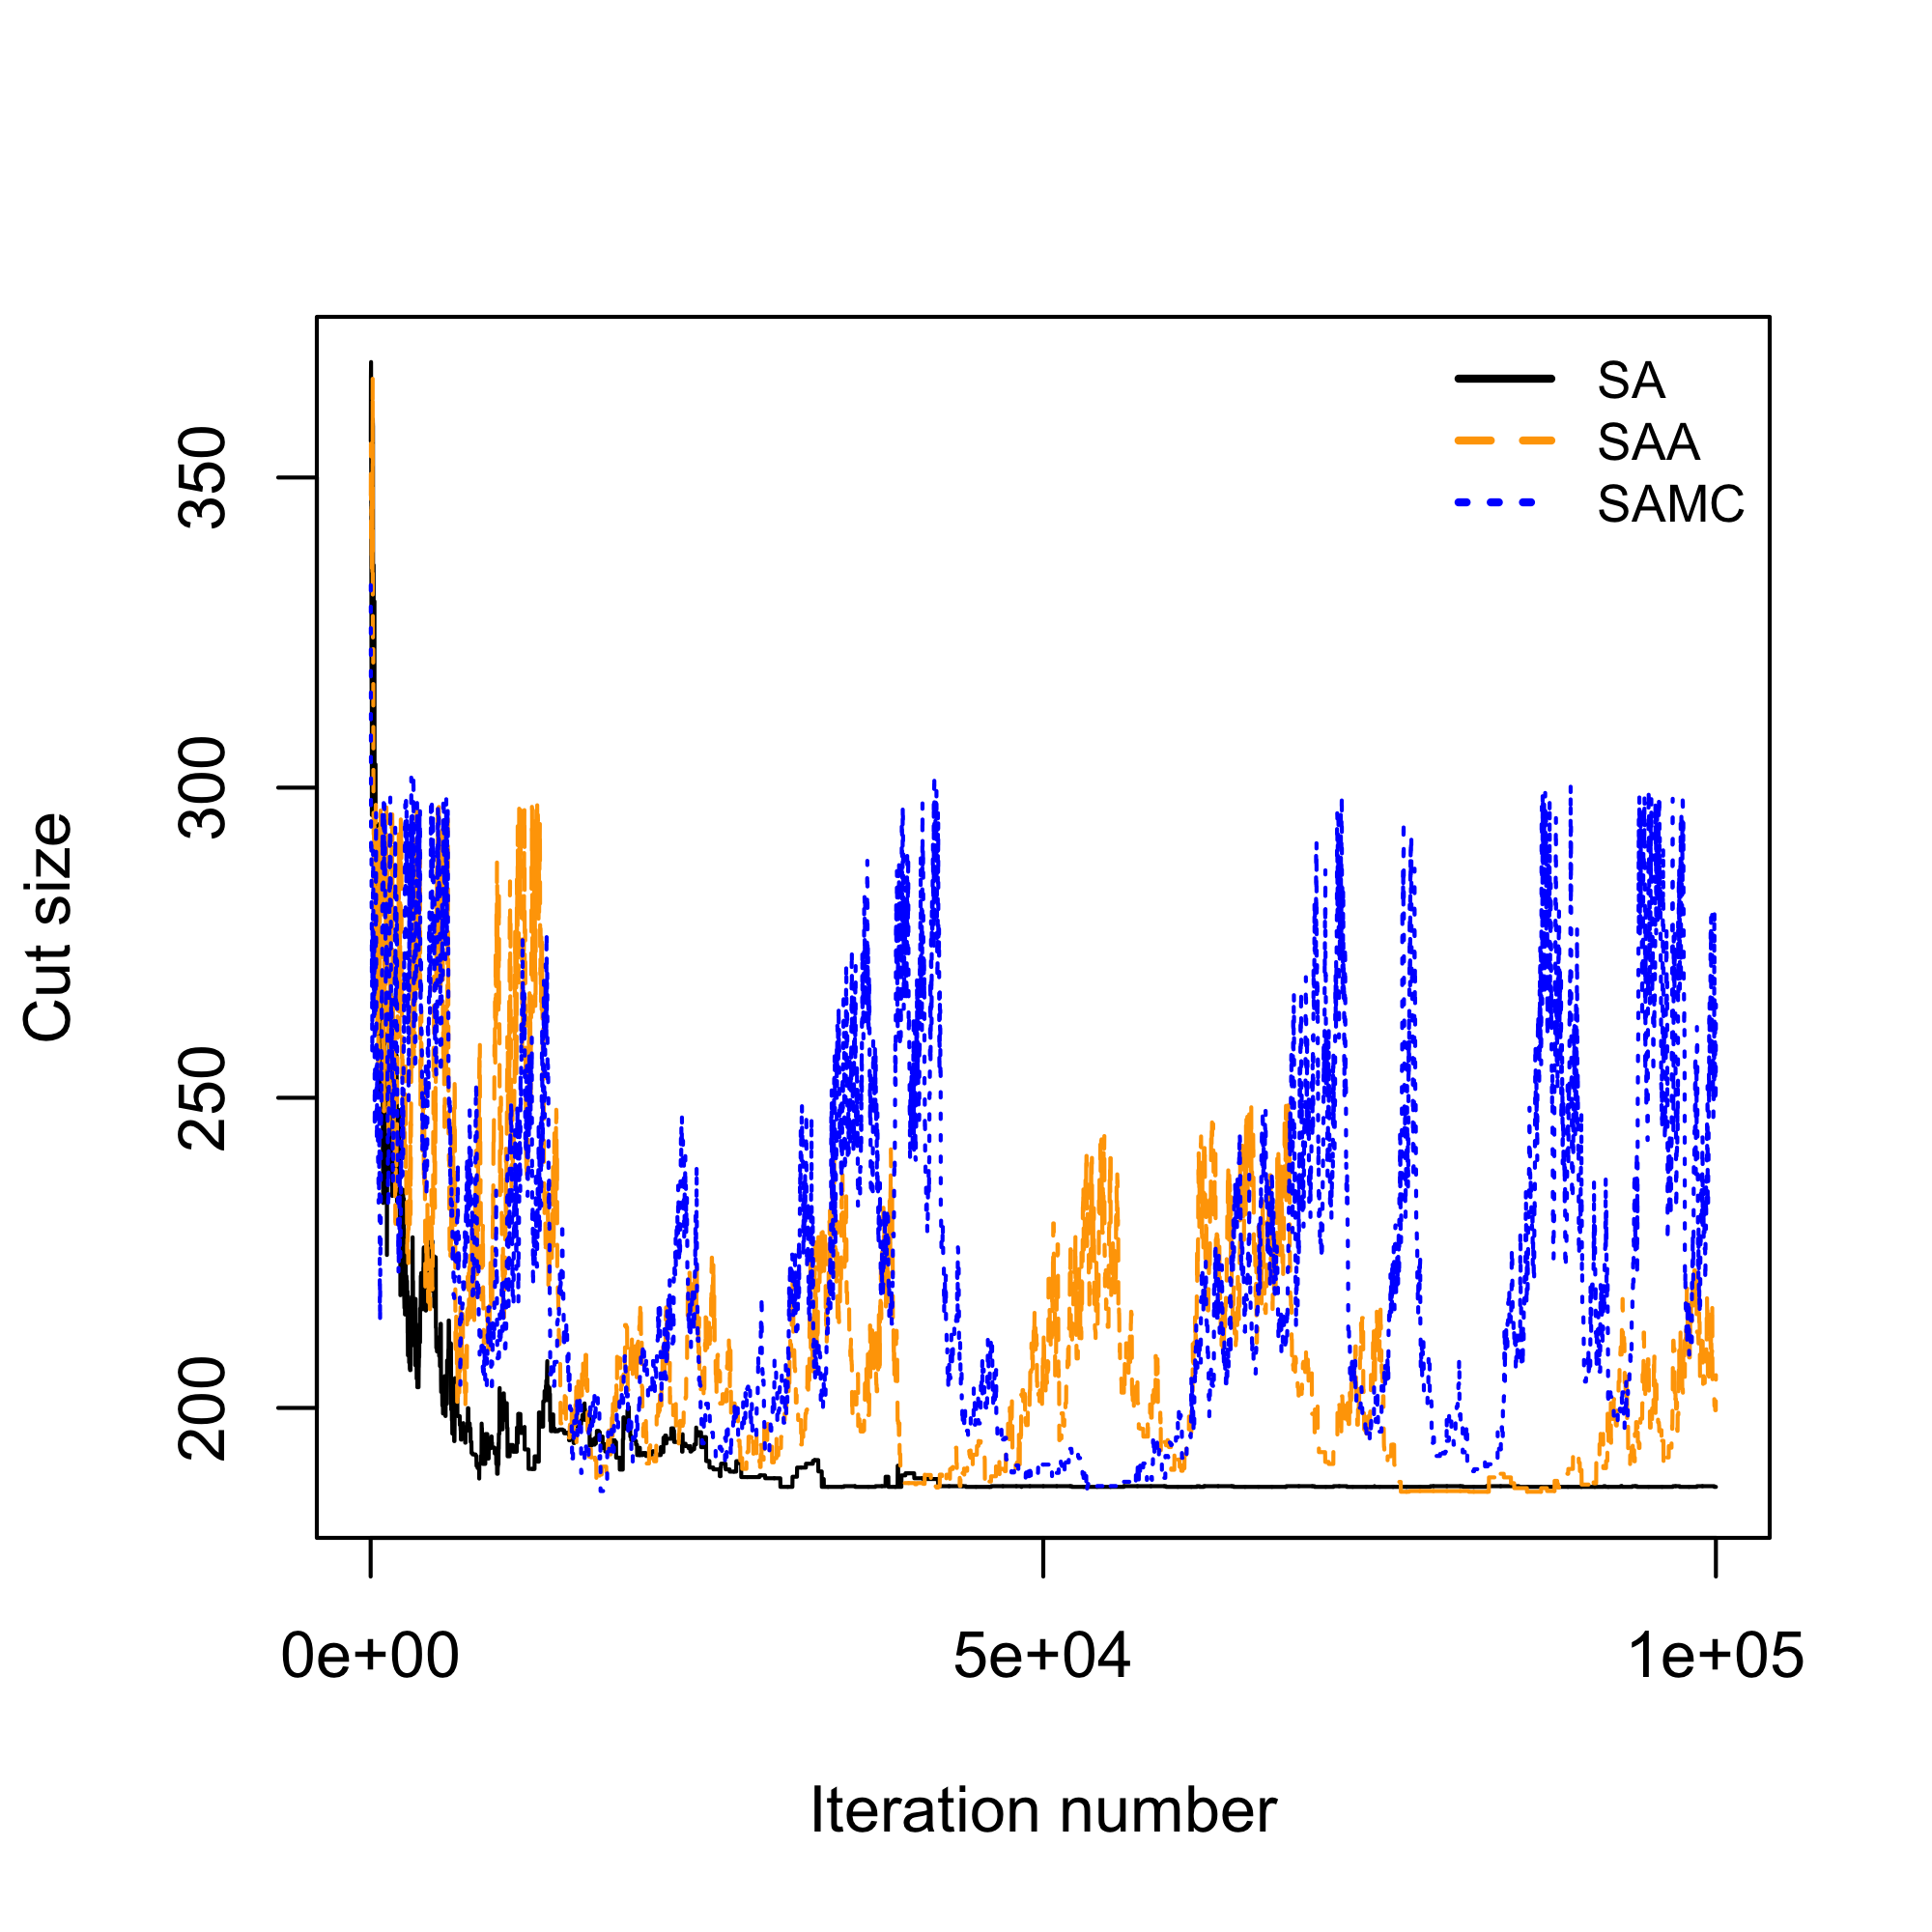
\includegraphics[width=.5\textwidth]{images/graph_cut_n100_iter1e+05}
    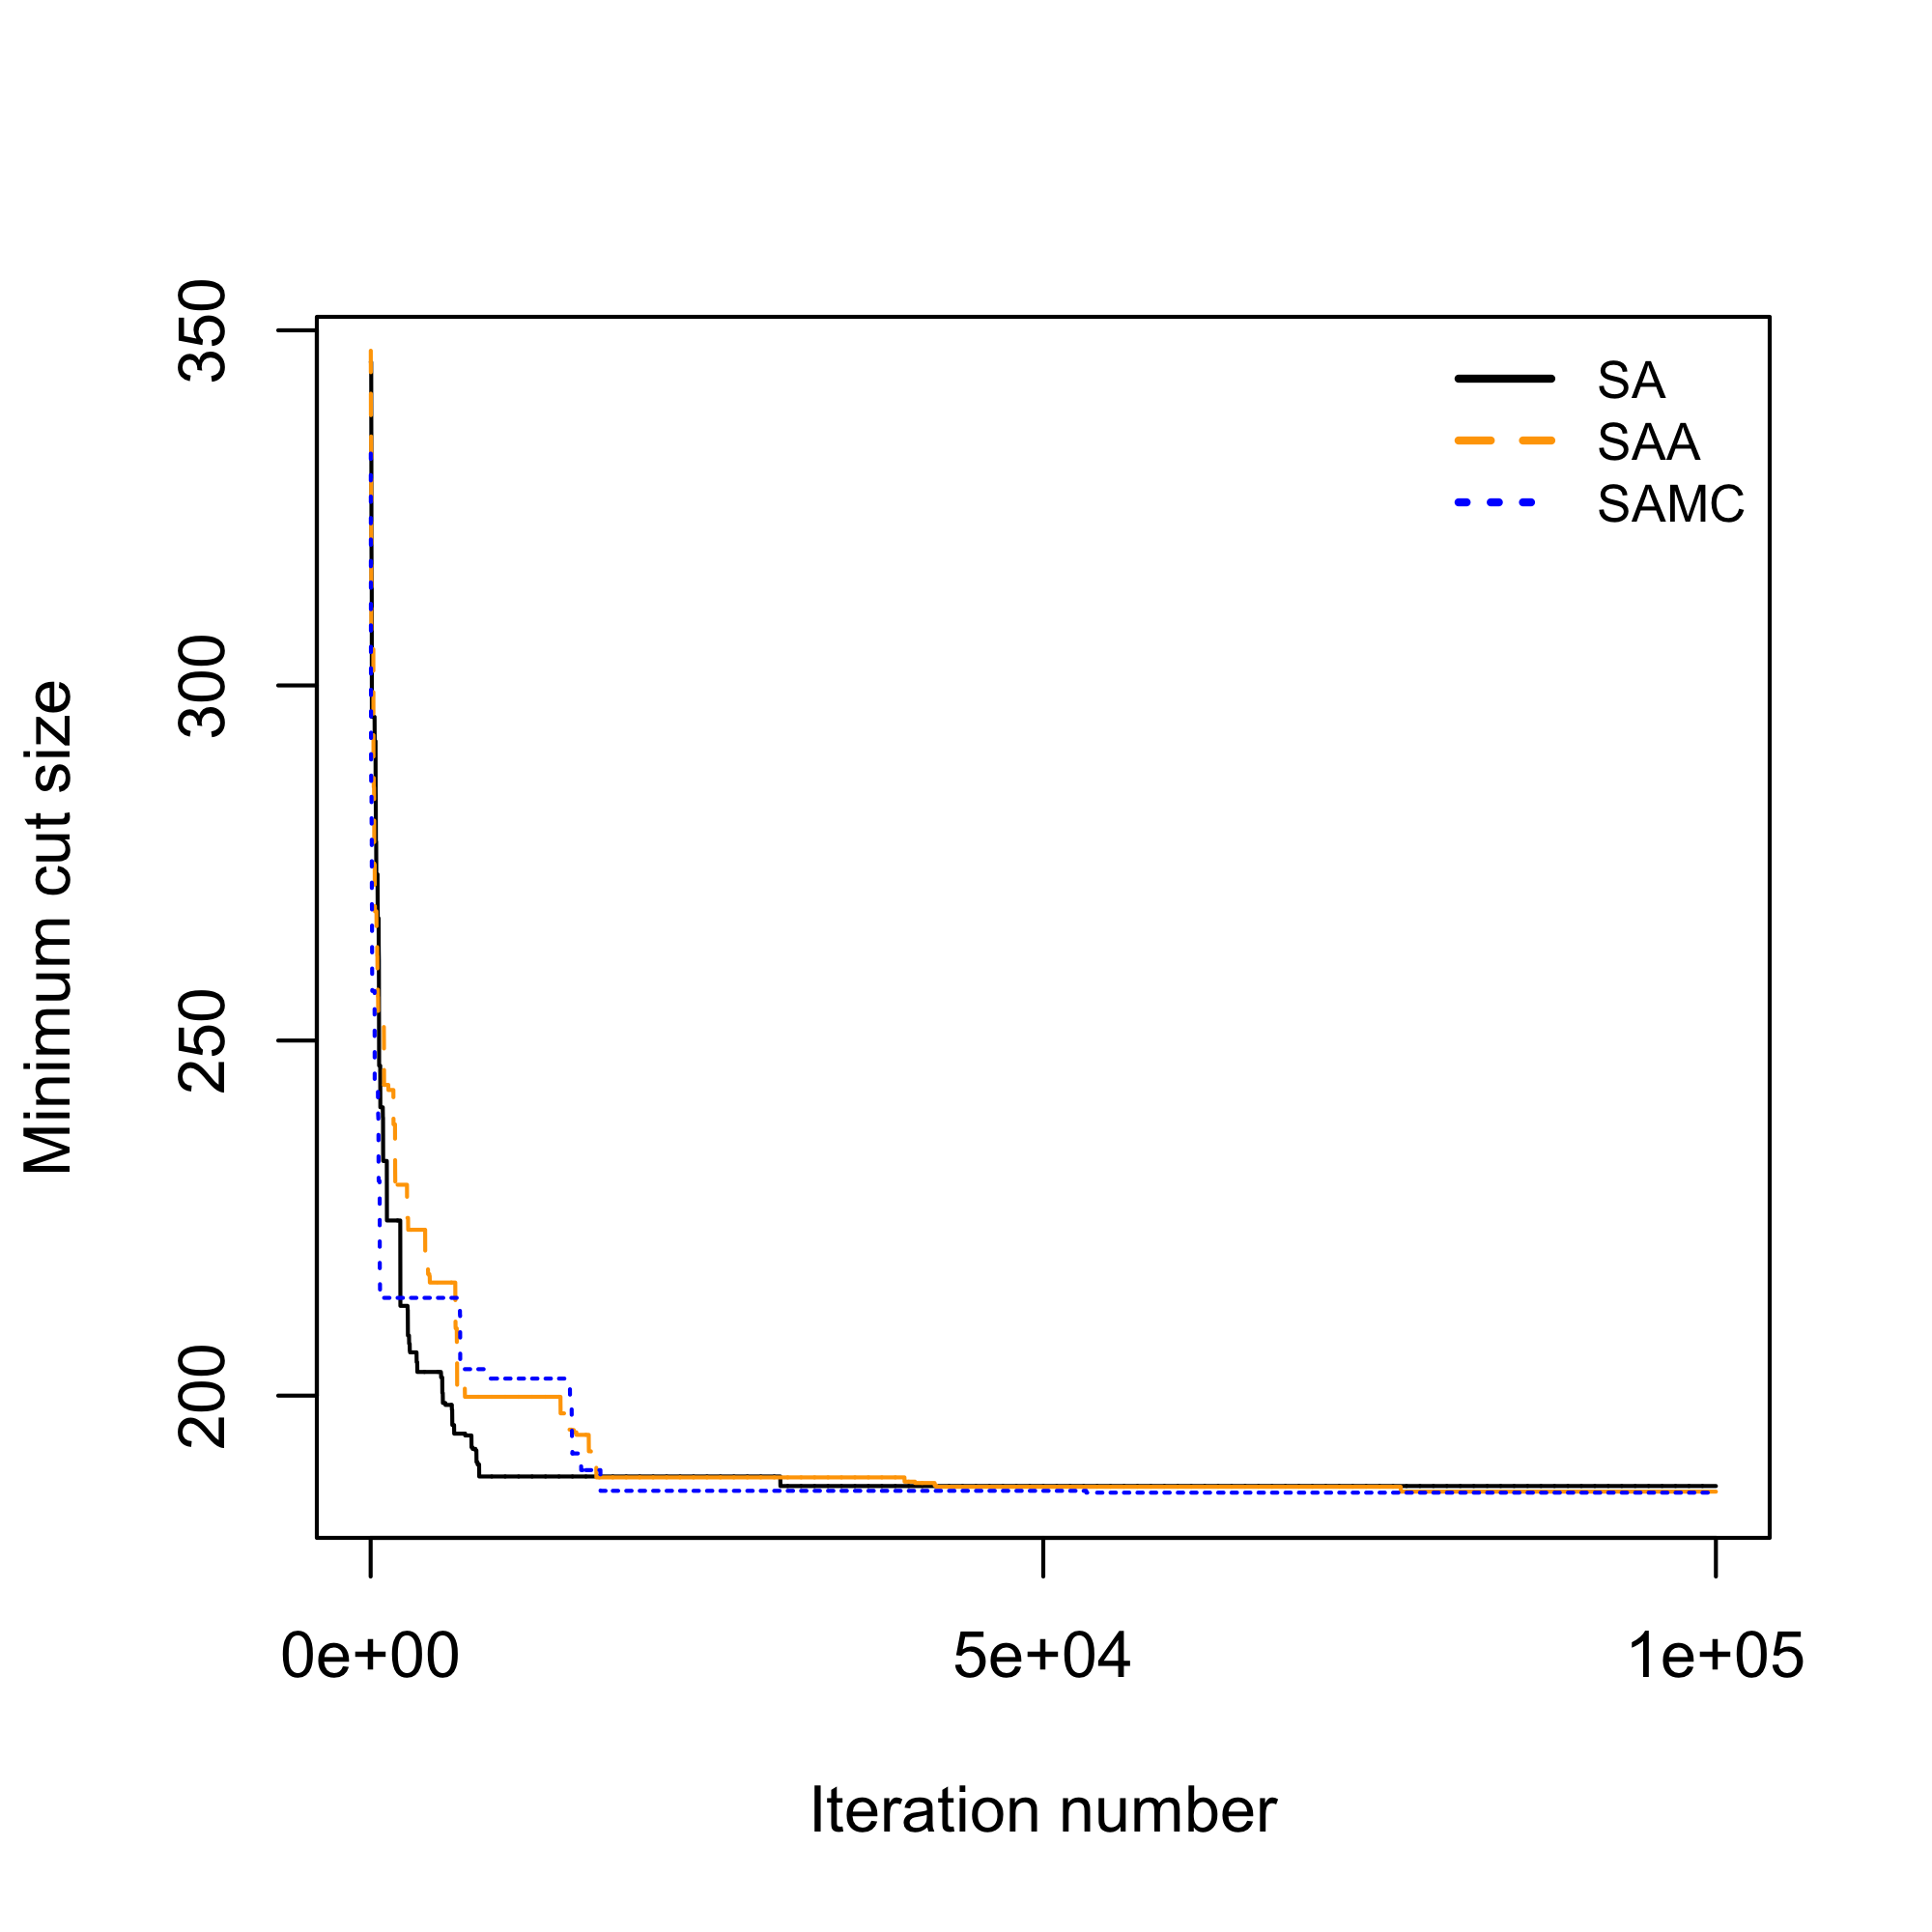
\includegraphics[width=.5\textwidth]{images/graph_min_cut_n100_iter1e+05}
  \end{tabular}
  \caption{Comparison of SA, SAA, and SAMC for $n = 100$}
  \label{fig:n100}
\end{figure}

\begin{figure}[hbpt]
  \begin{tabular}{cc}
    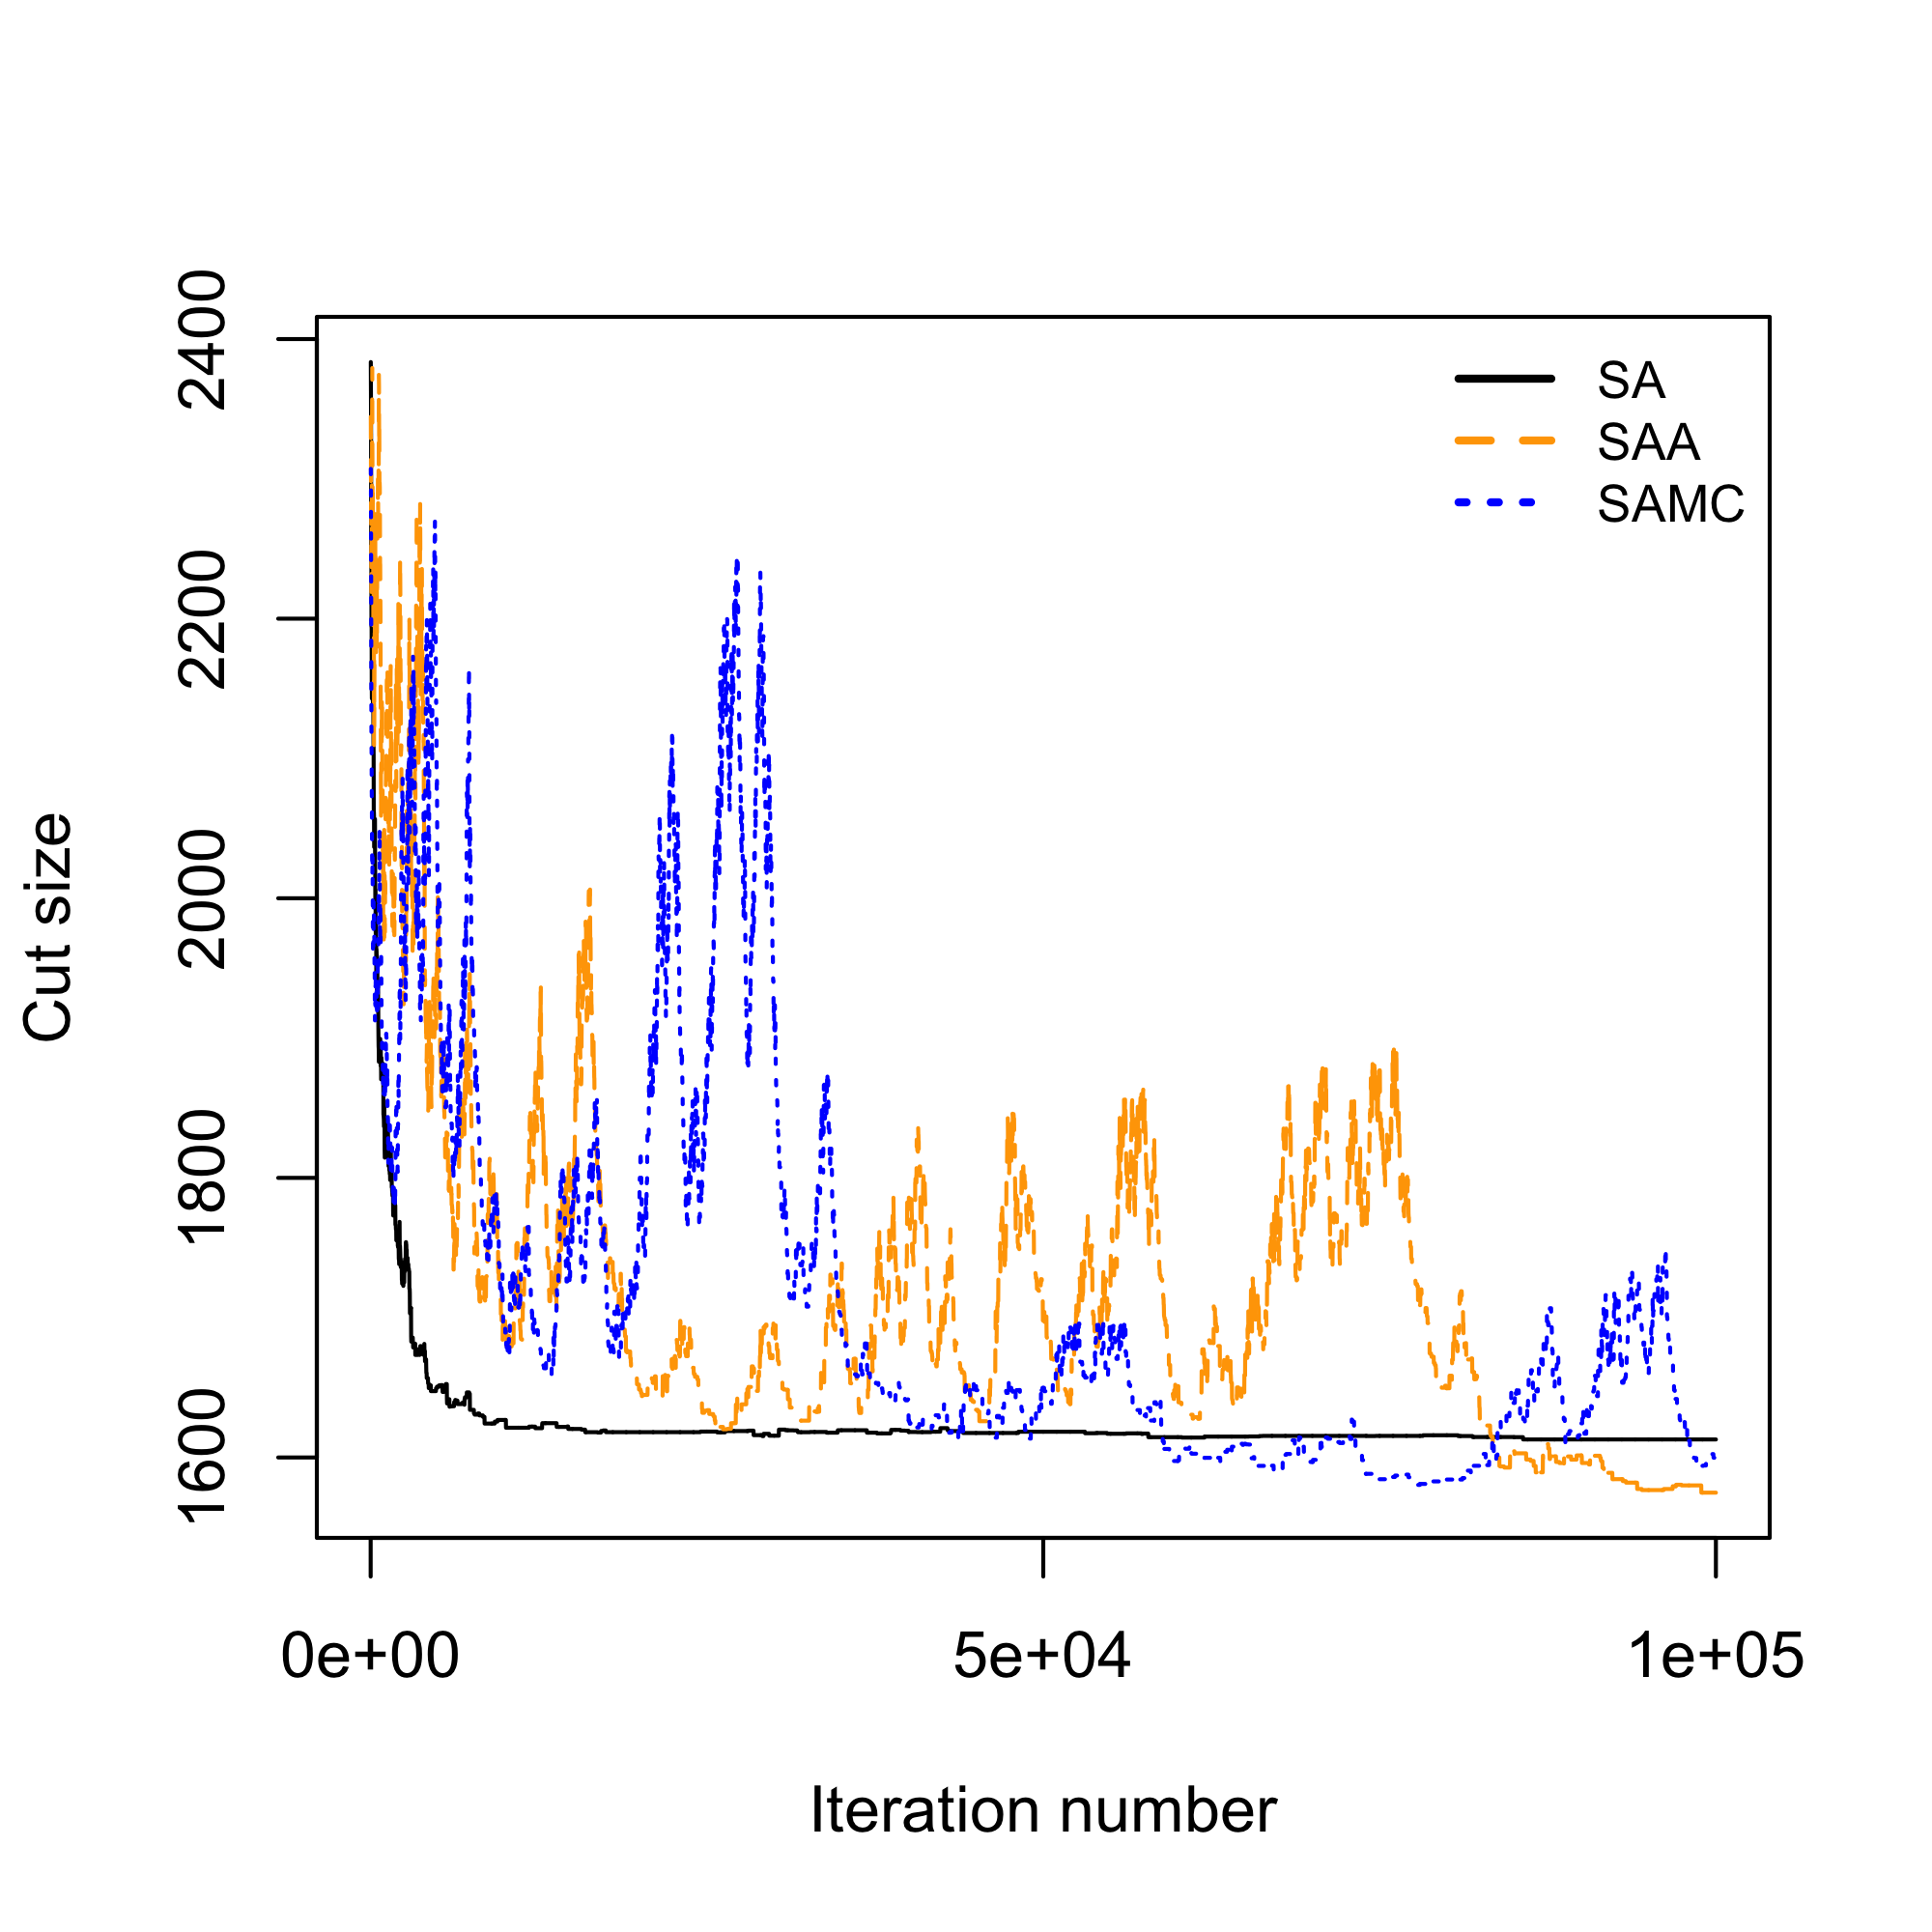
\includegraphics[width=.5\textwidth]{images/graph_cut_n250_iter1e+05}
    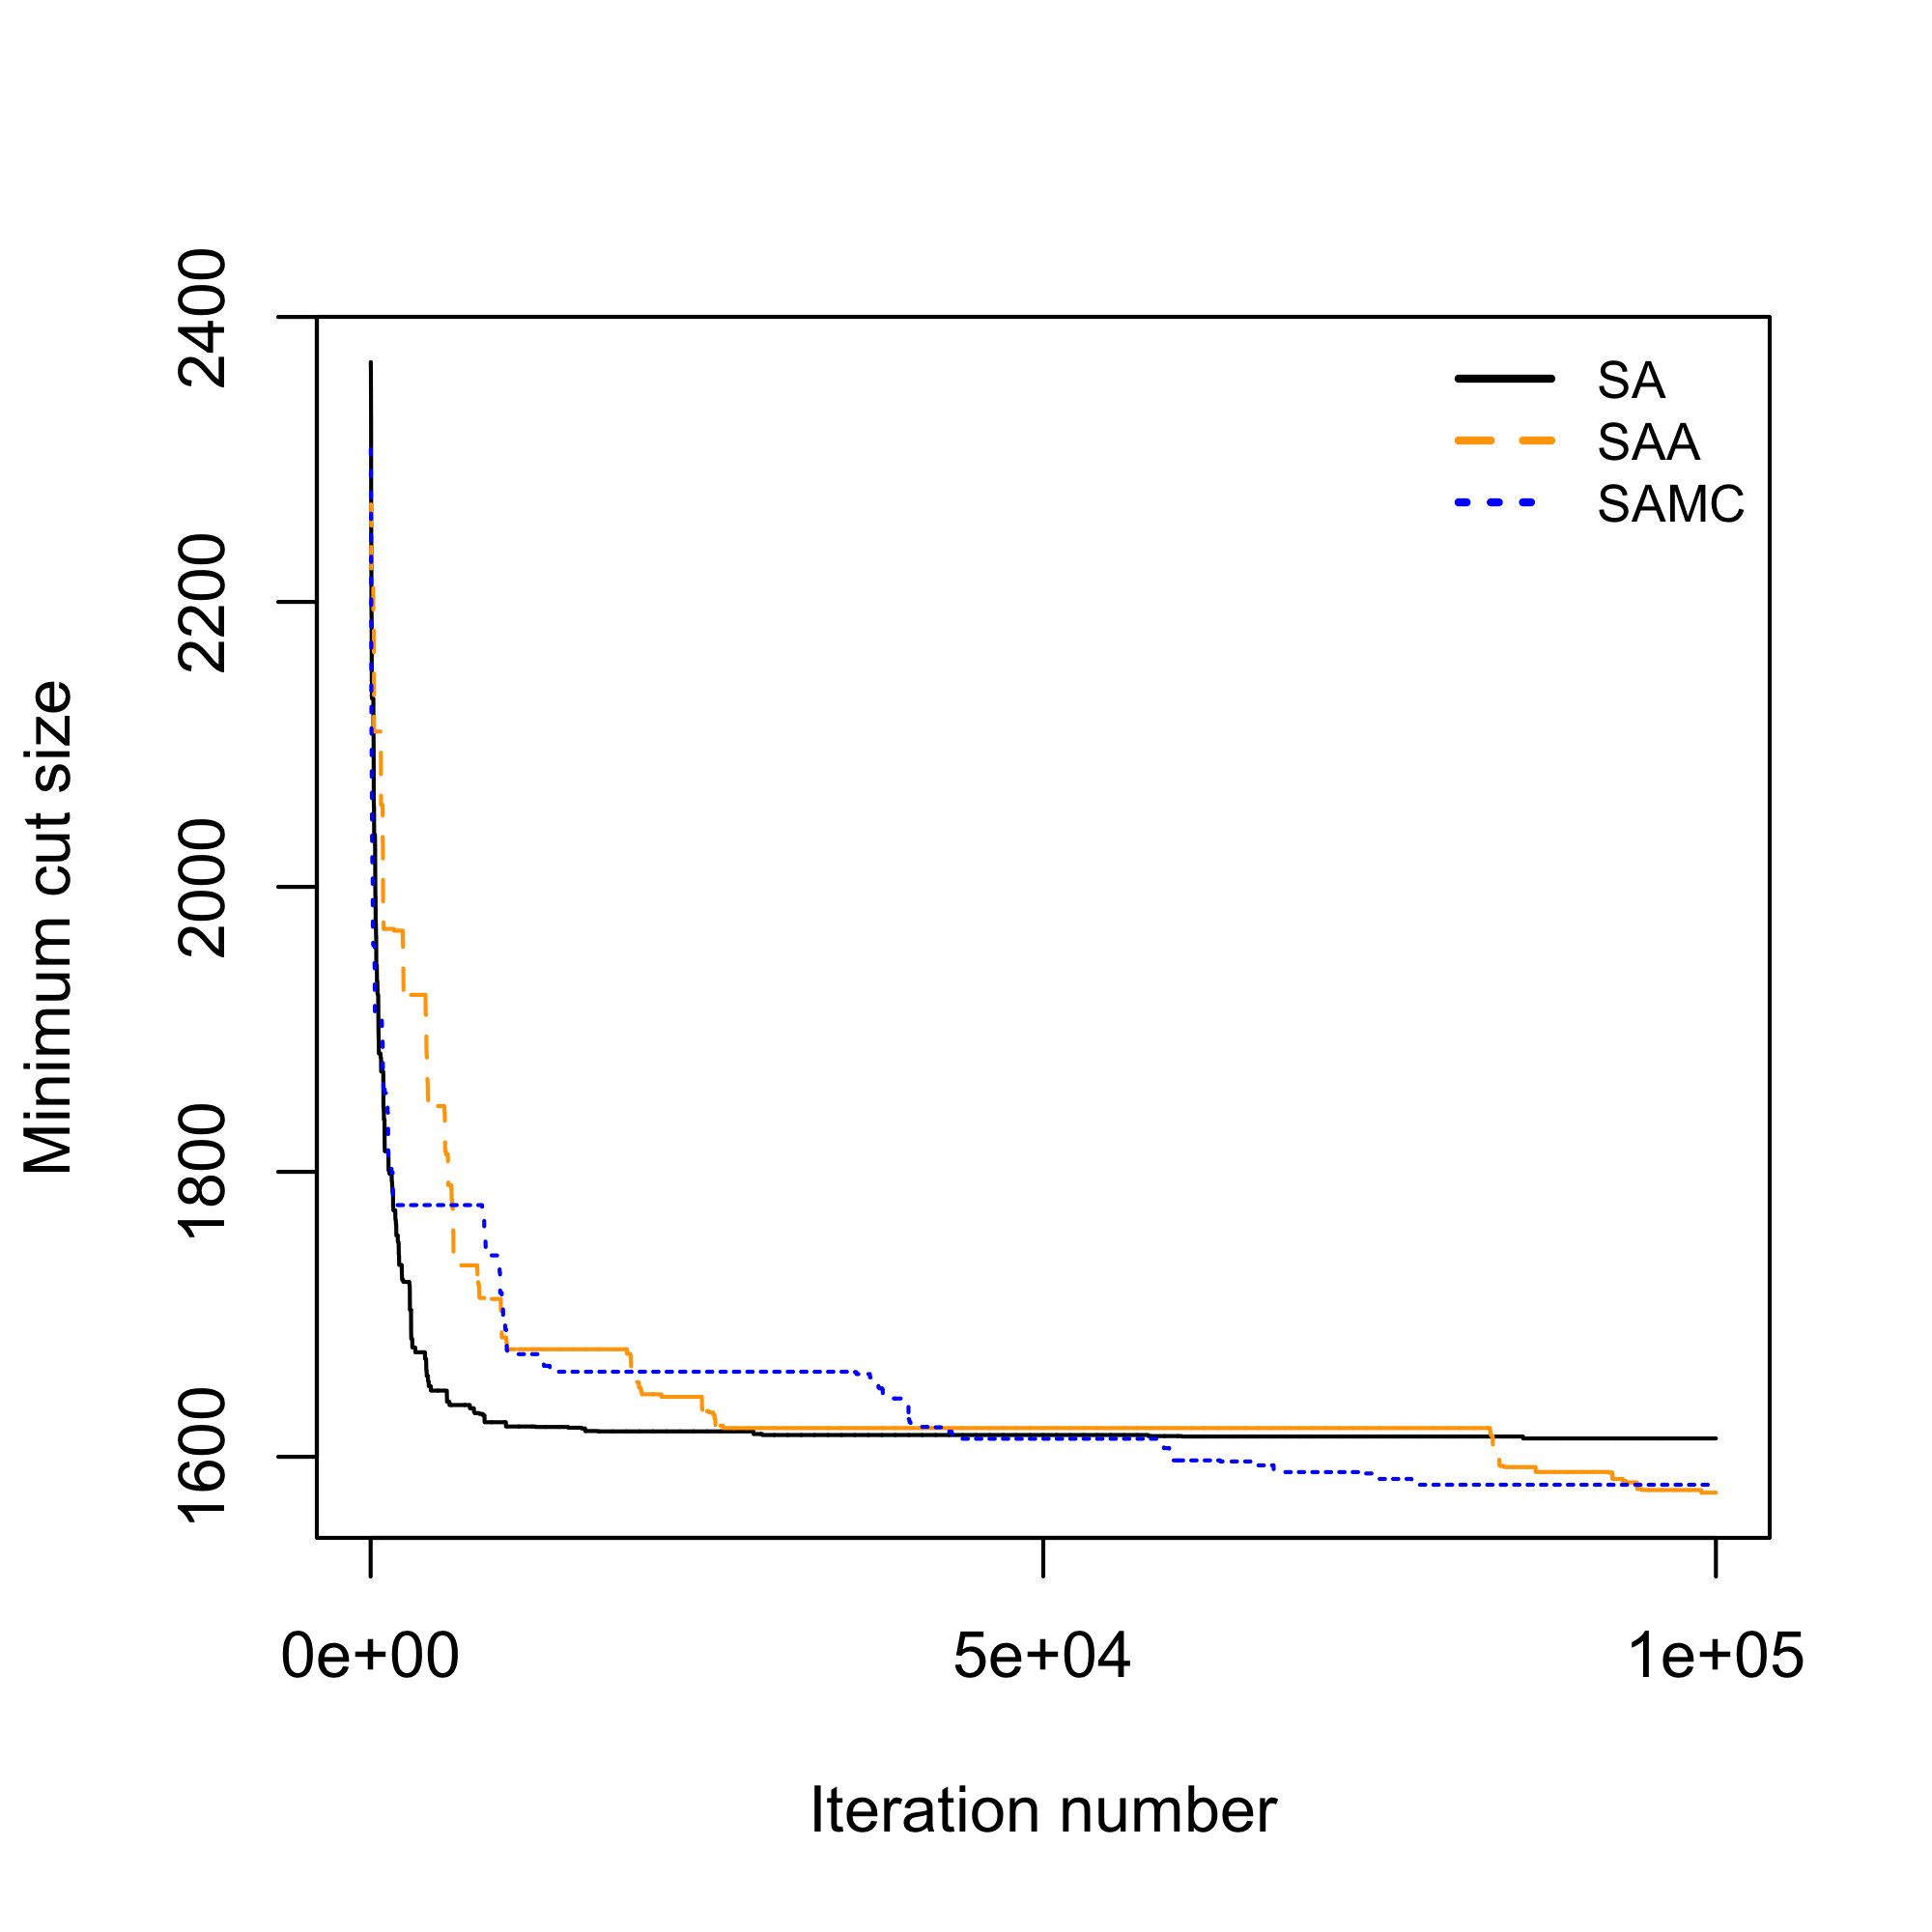
\includegraphics[width=.5\textwidth]{images/graph_min_cut_n250_iter1e+05}
  \end{tabular}
  \caption{Comparison of SA, SAA, and SAMC for $n = 250$}
  \label{fig:n250}
\end{figure}

\begin{figure}[hbpt]
  \begin{tabular}{cc}
    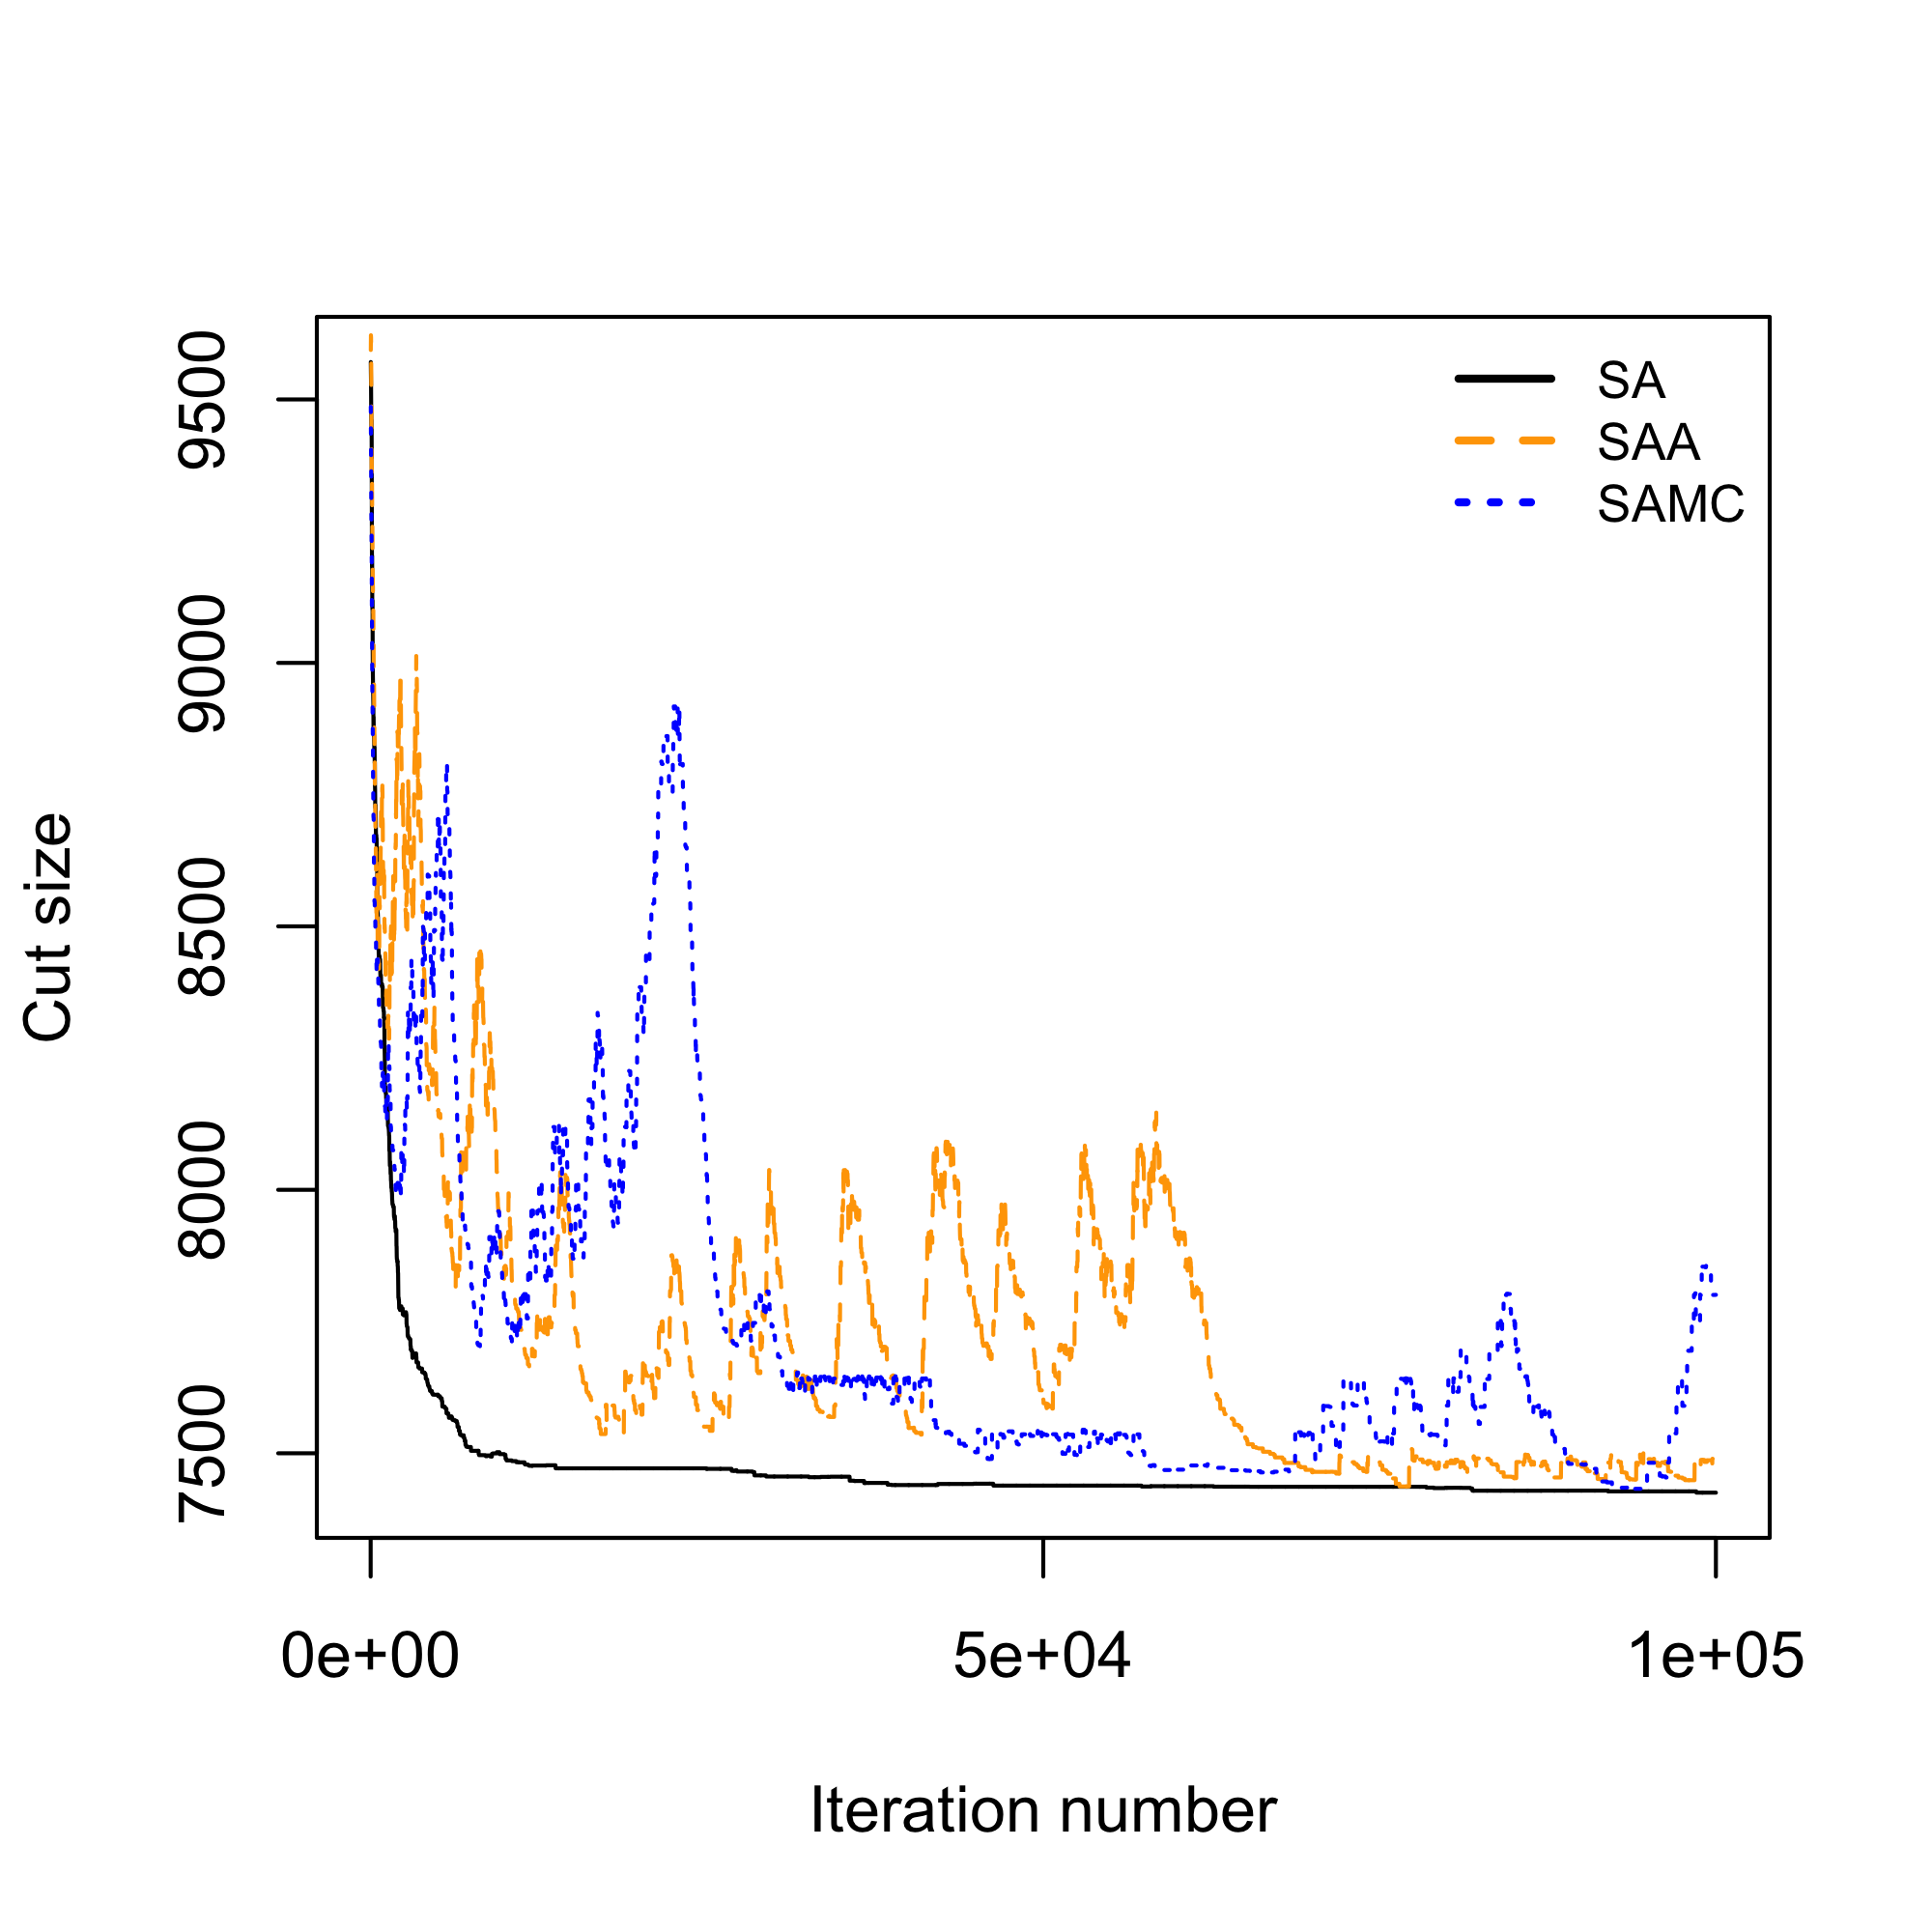
\includegraphics[width=.5\textwidth]{images/graph_cut_n500_iter1e+05}
    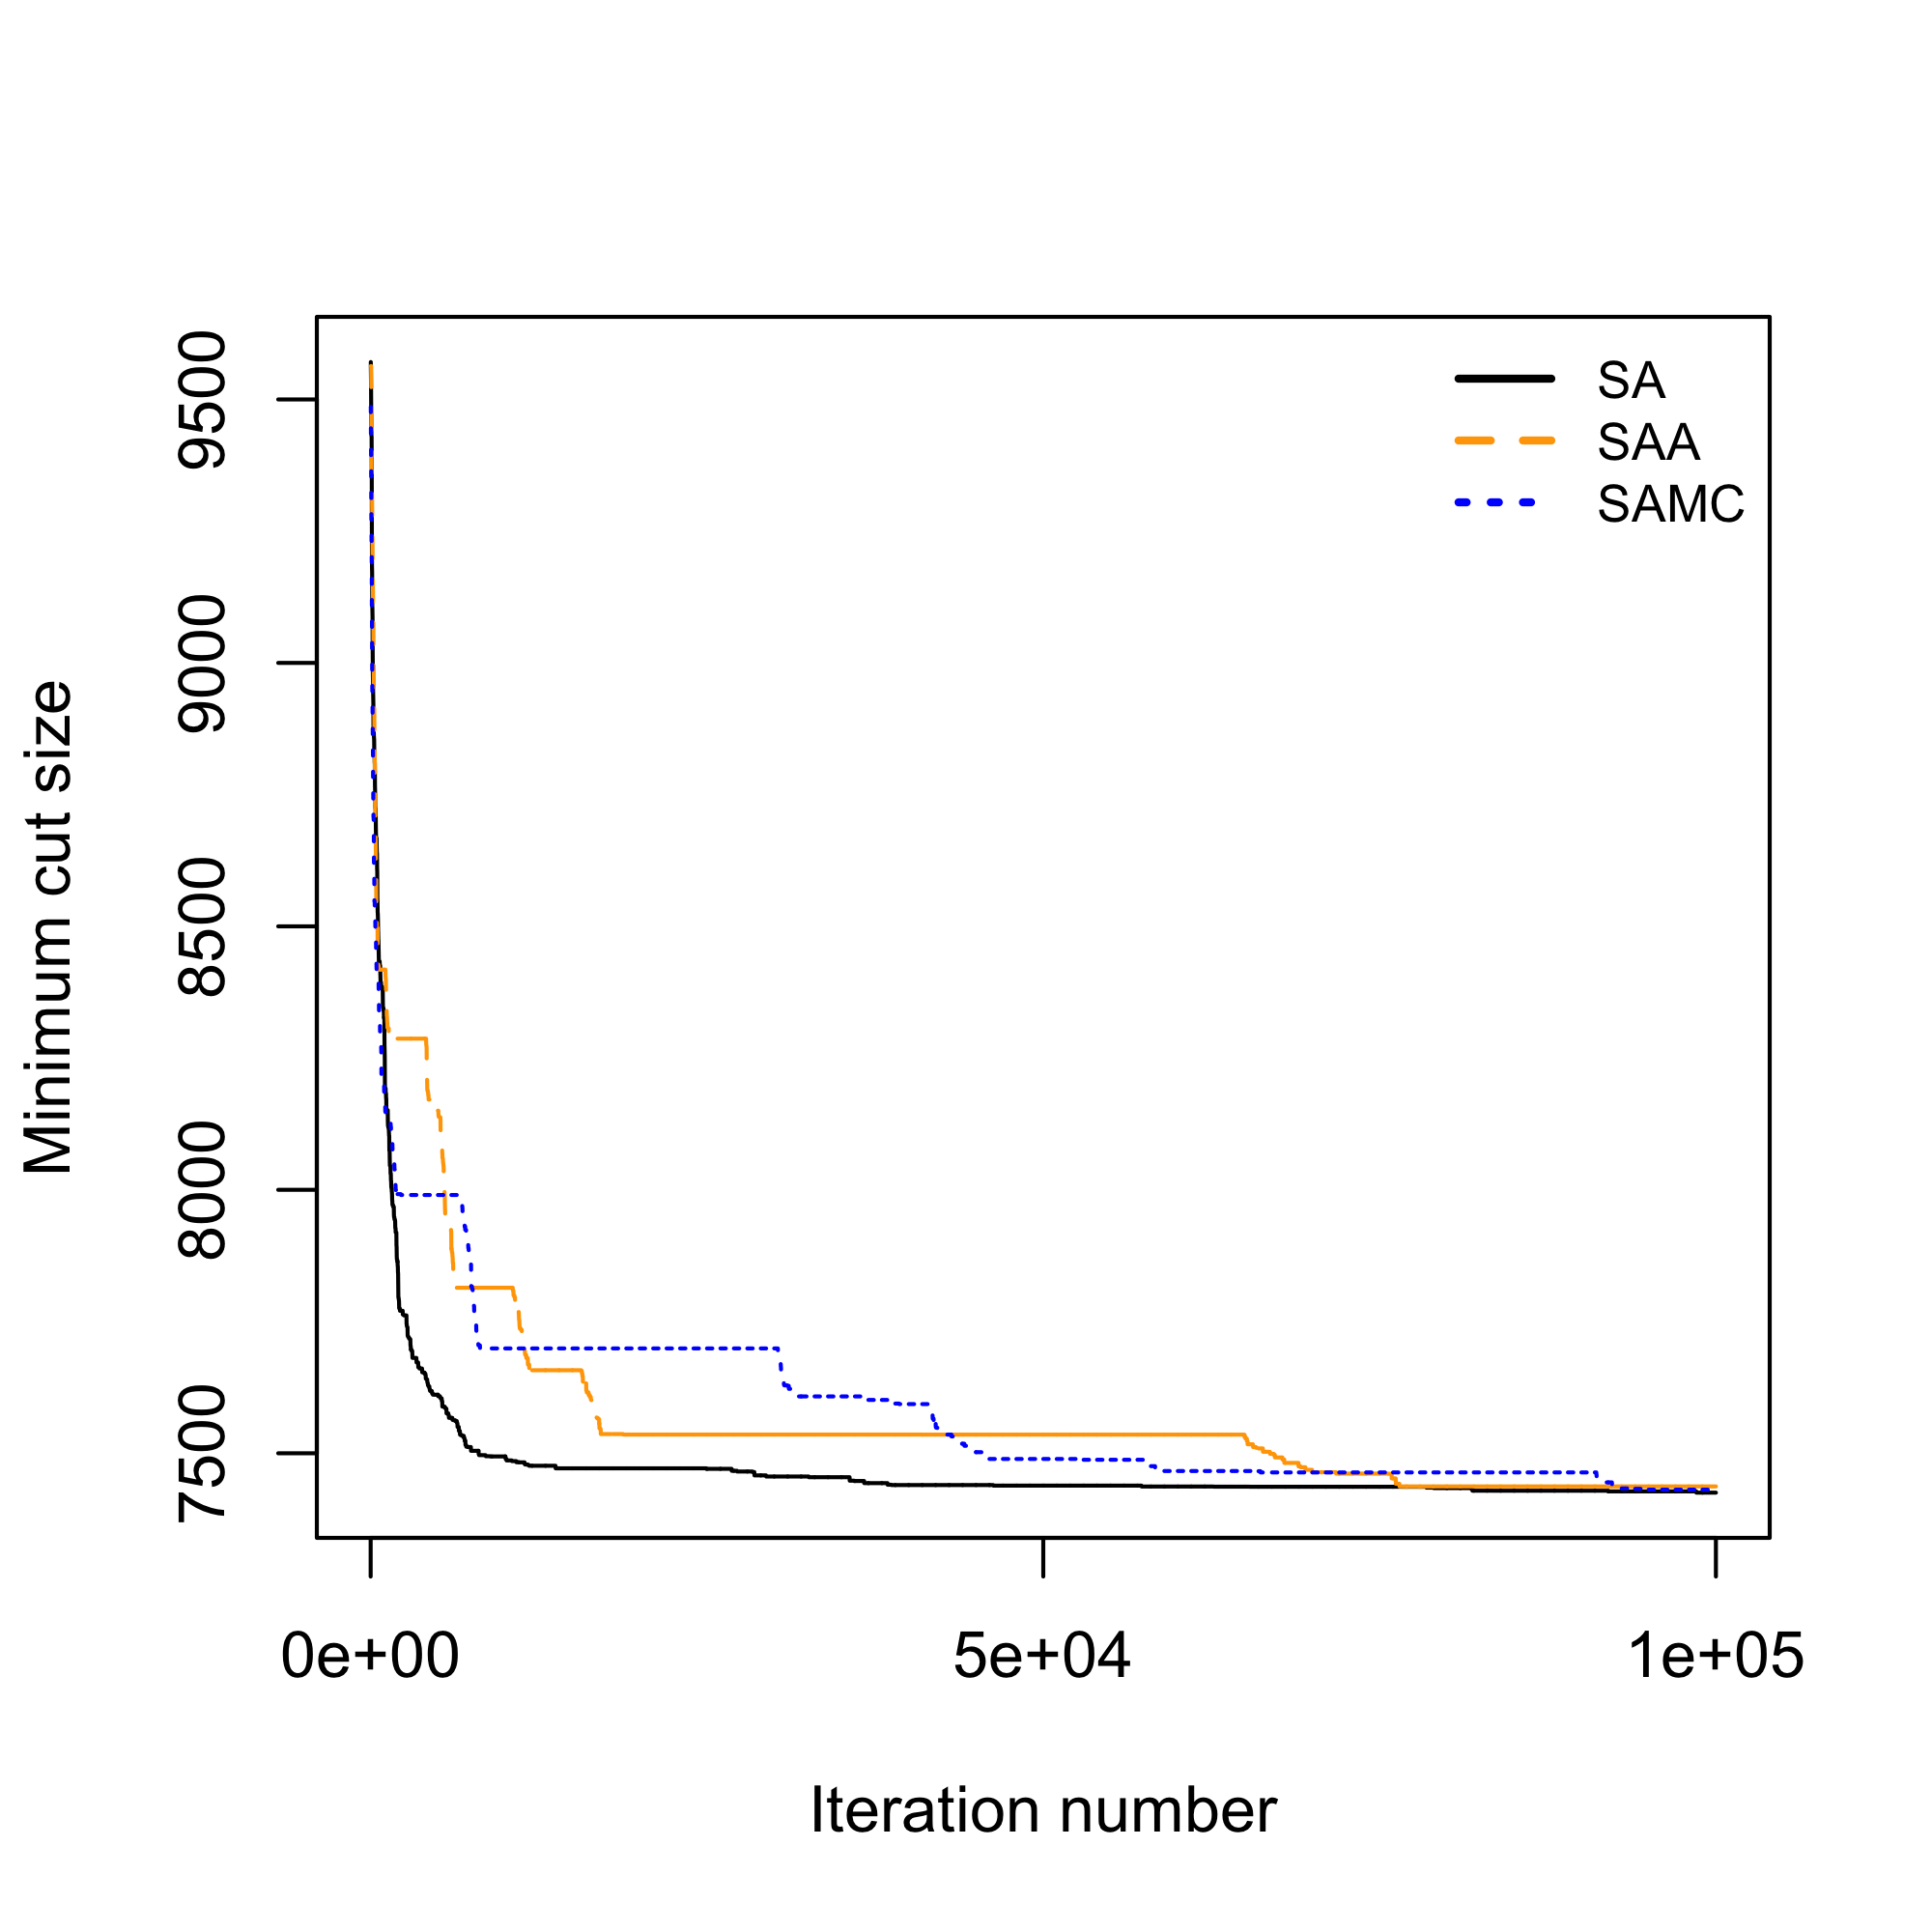
\includegraphics[width=.5\textwidth]{images/graph_min_cut_n500_iter1e+05}
  \end{tabular}
  \caption{Comparison of SA, SAA, and SAMC for $n = 500$}
  \label{fig:n500}
\end{figure}

\begin{figure}[hbpt]
  \begin{tabular}{cc}
    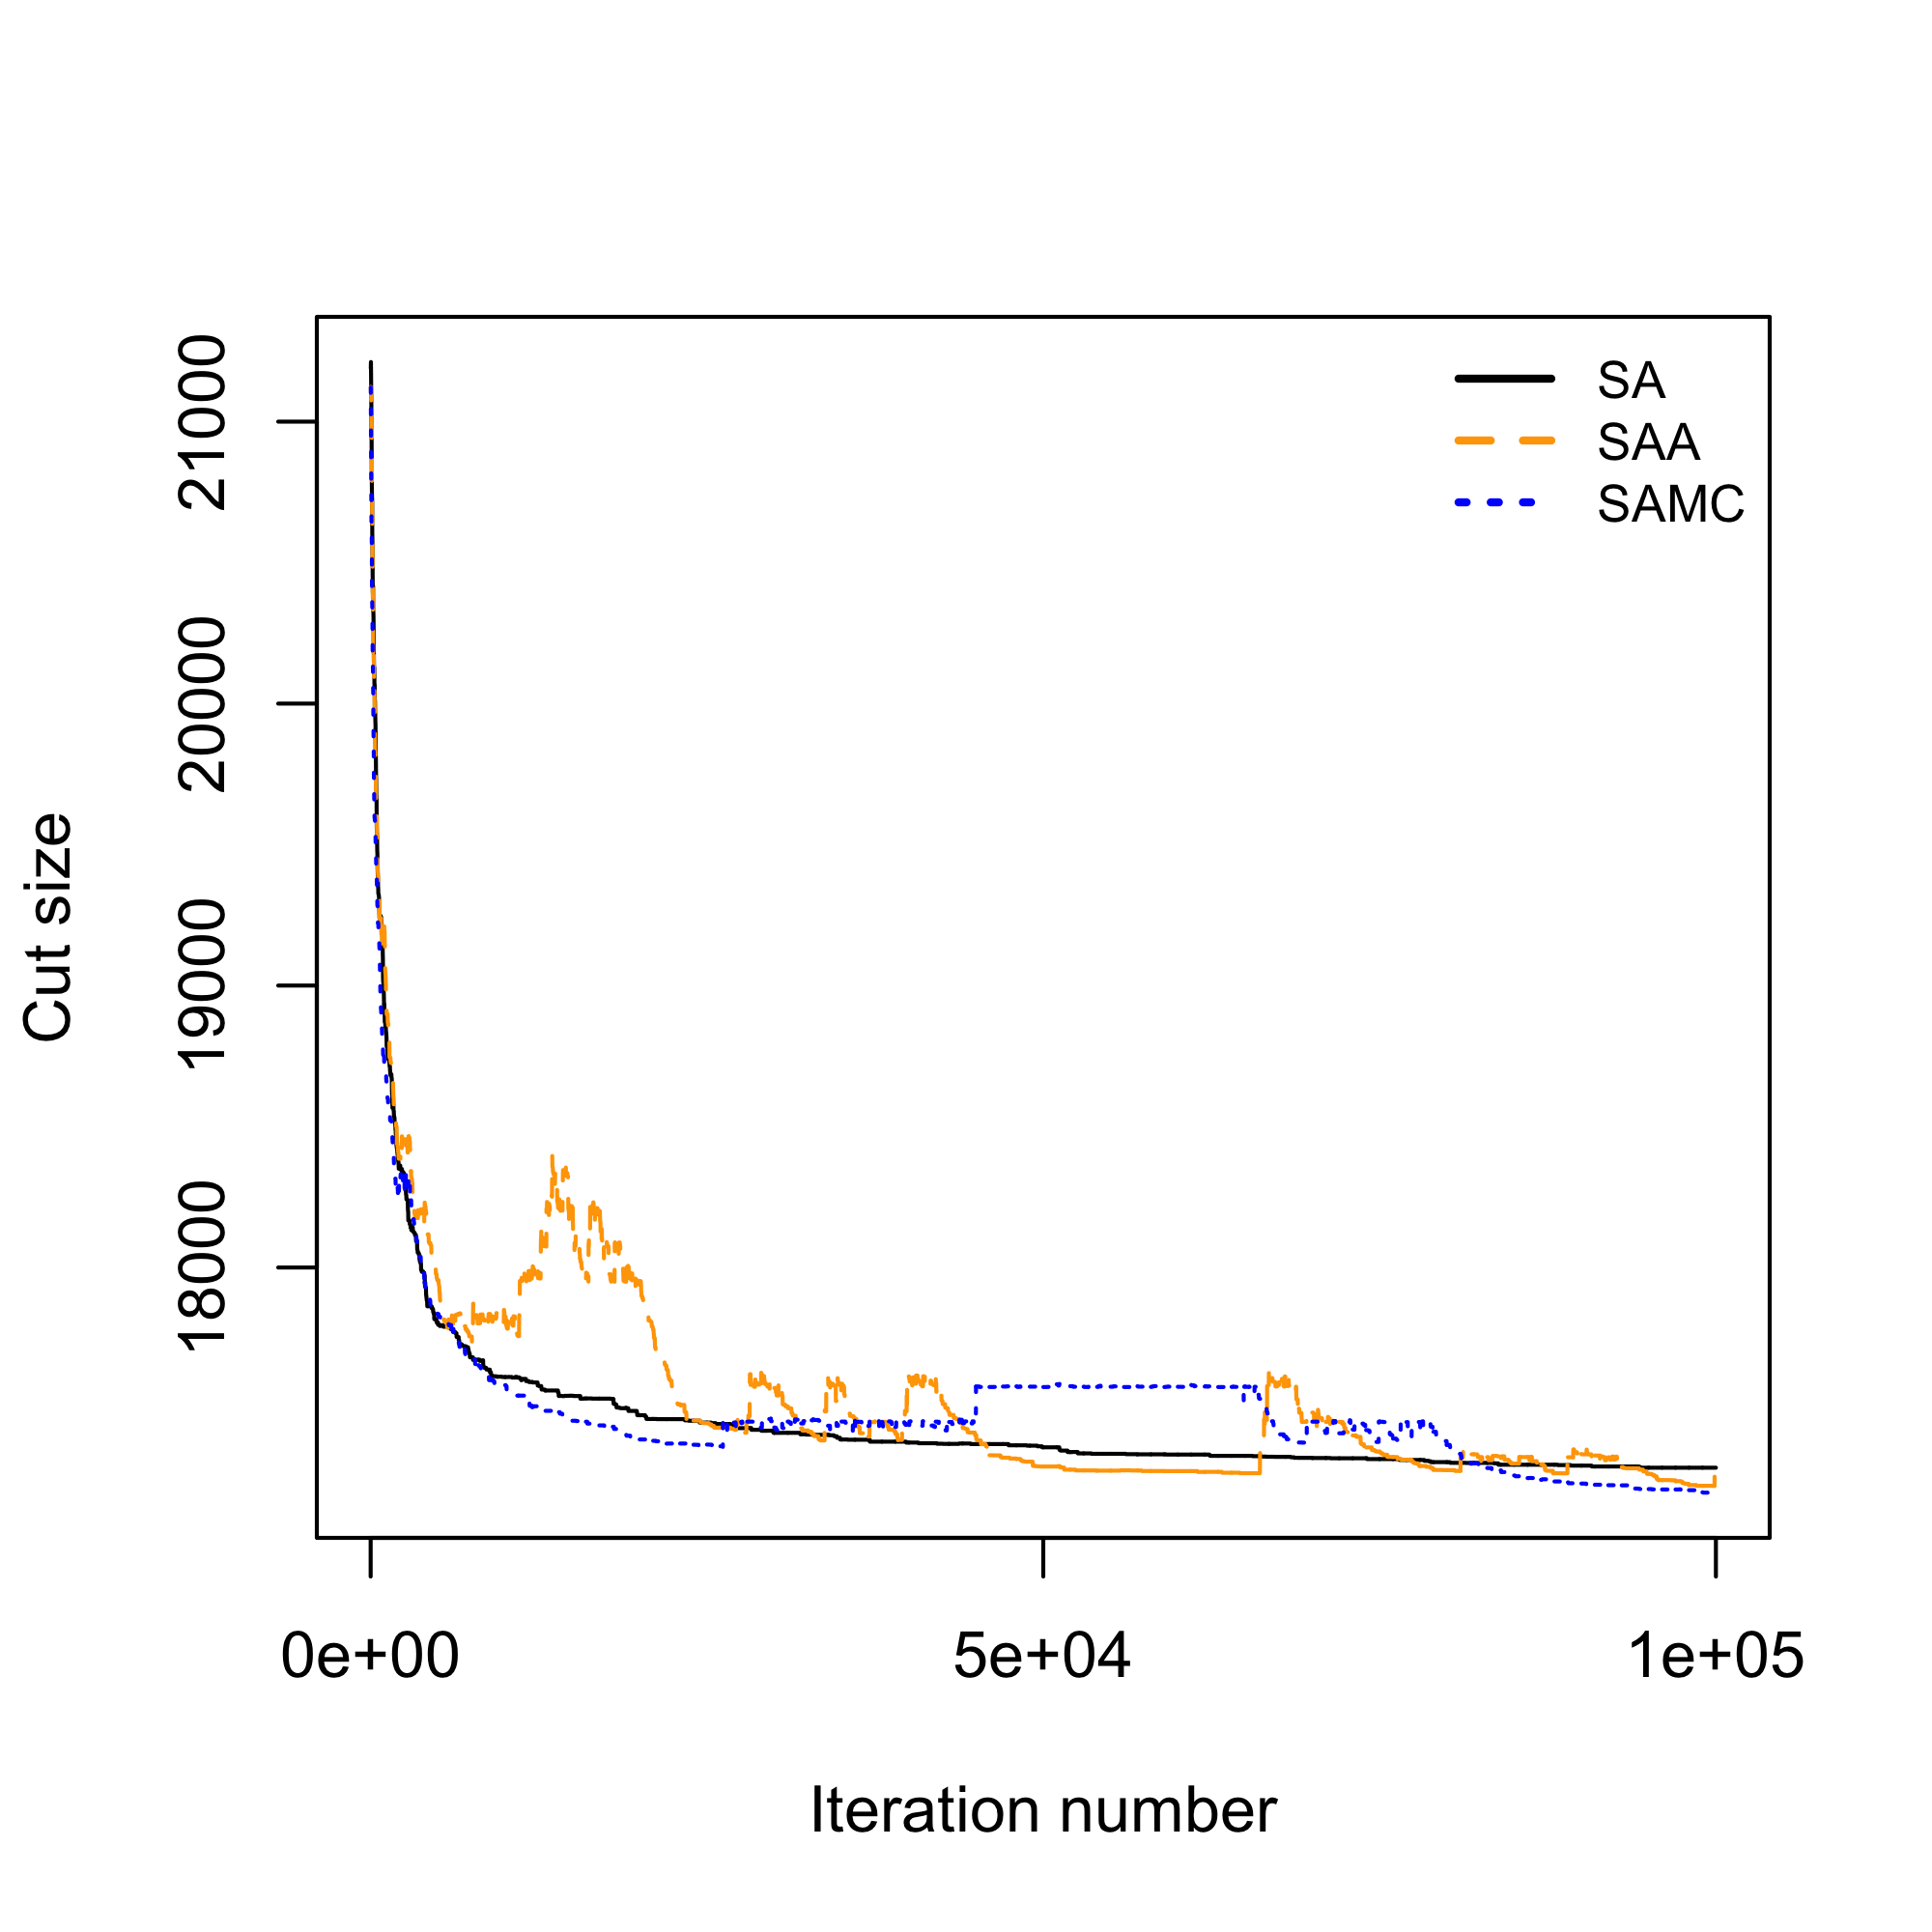
\includegraphics[width=.5\textwidth]{images/graph_cut_n750_iter1e+05}
    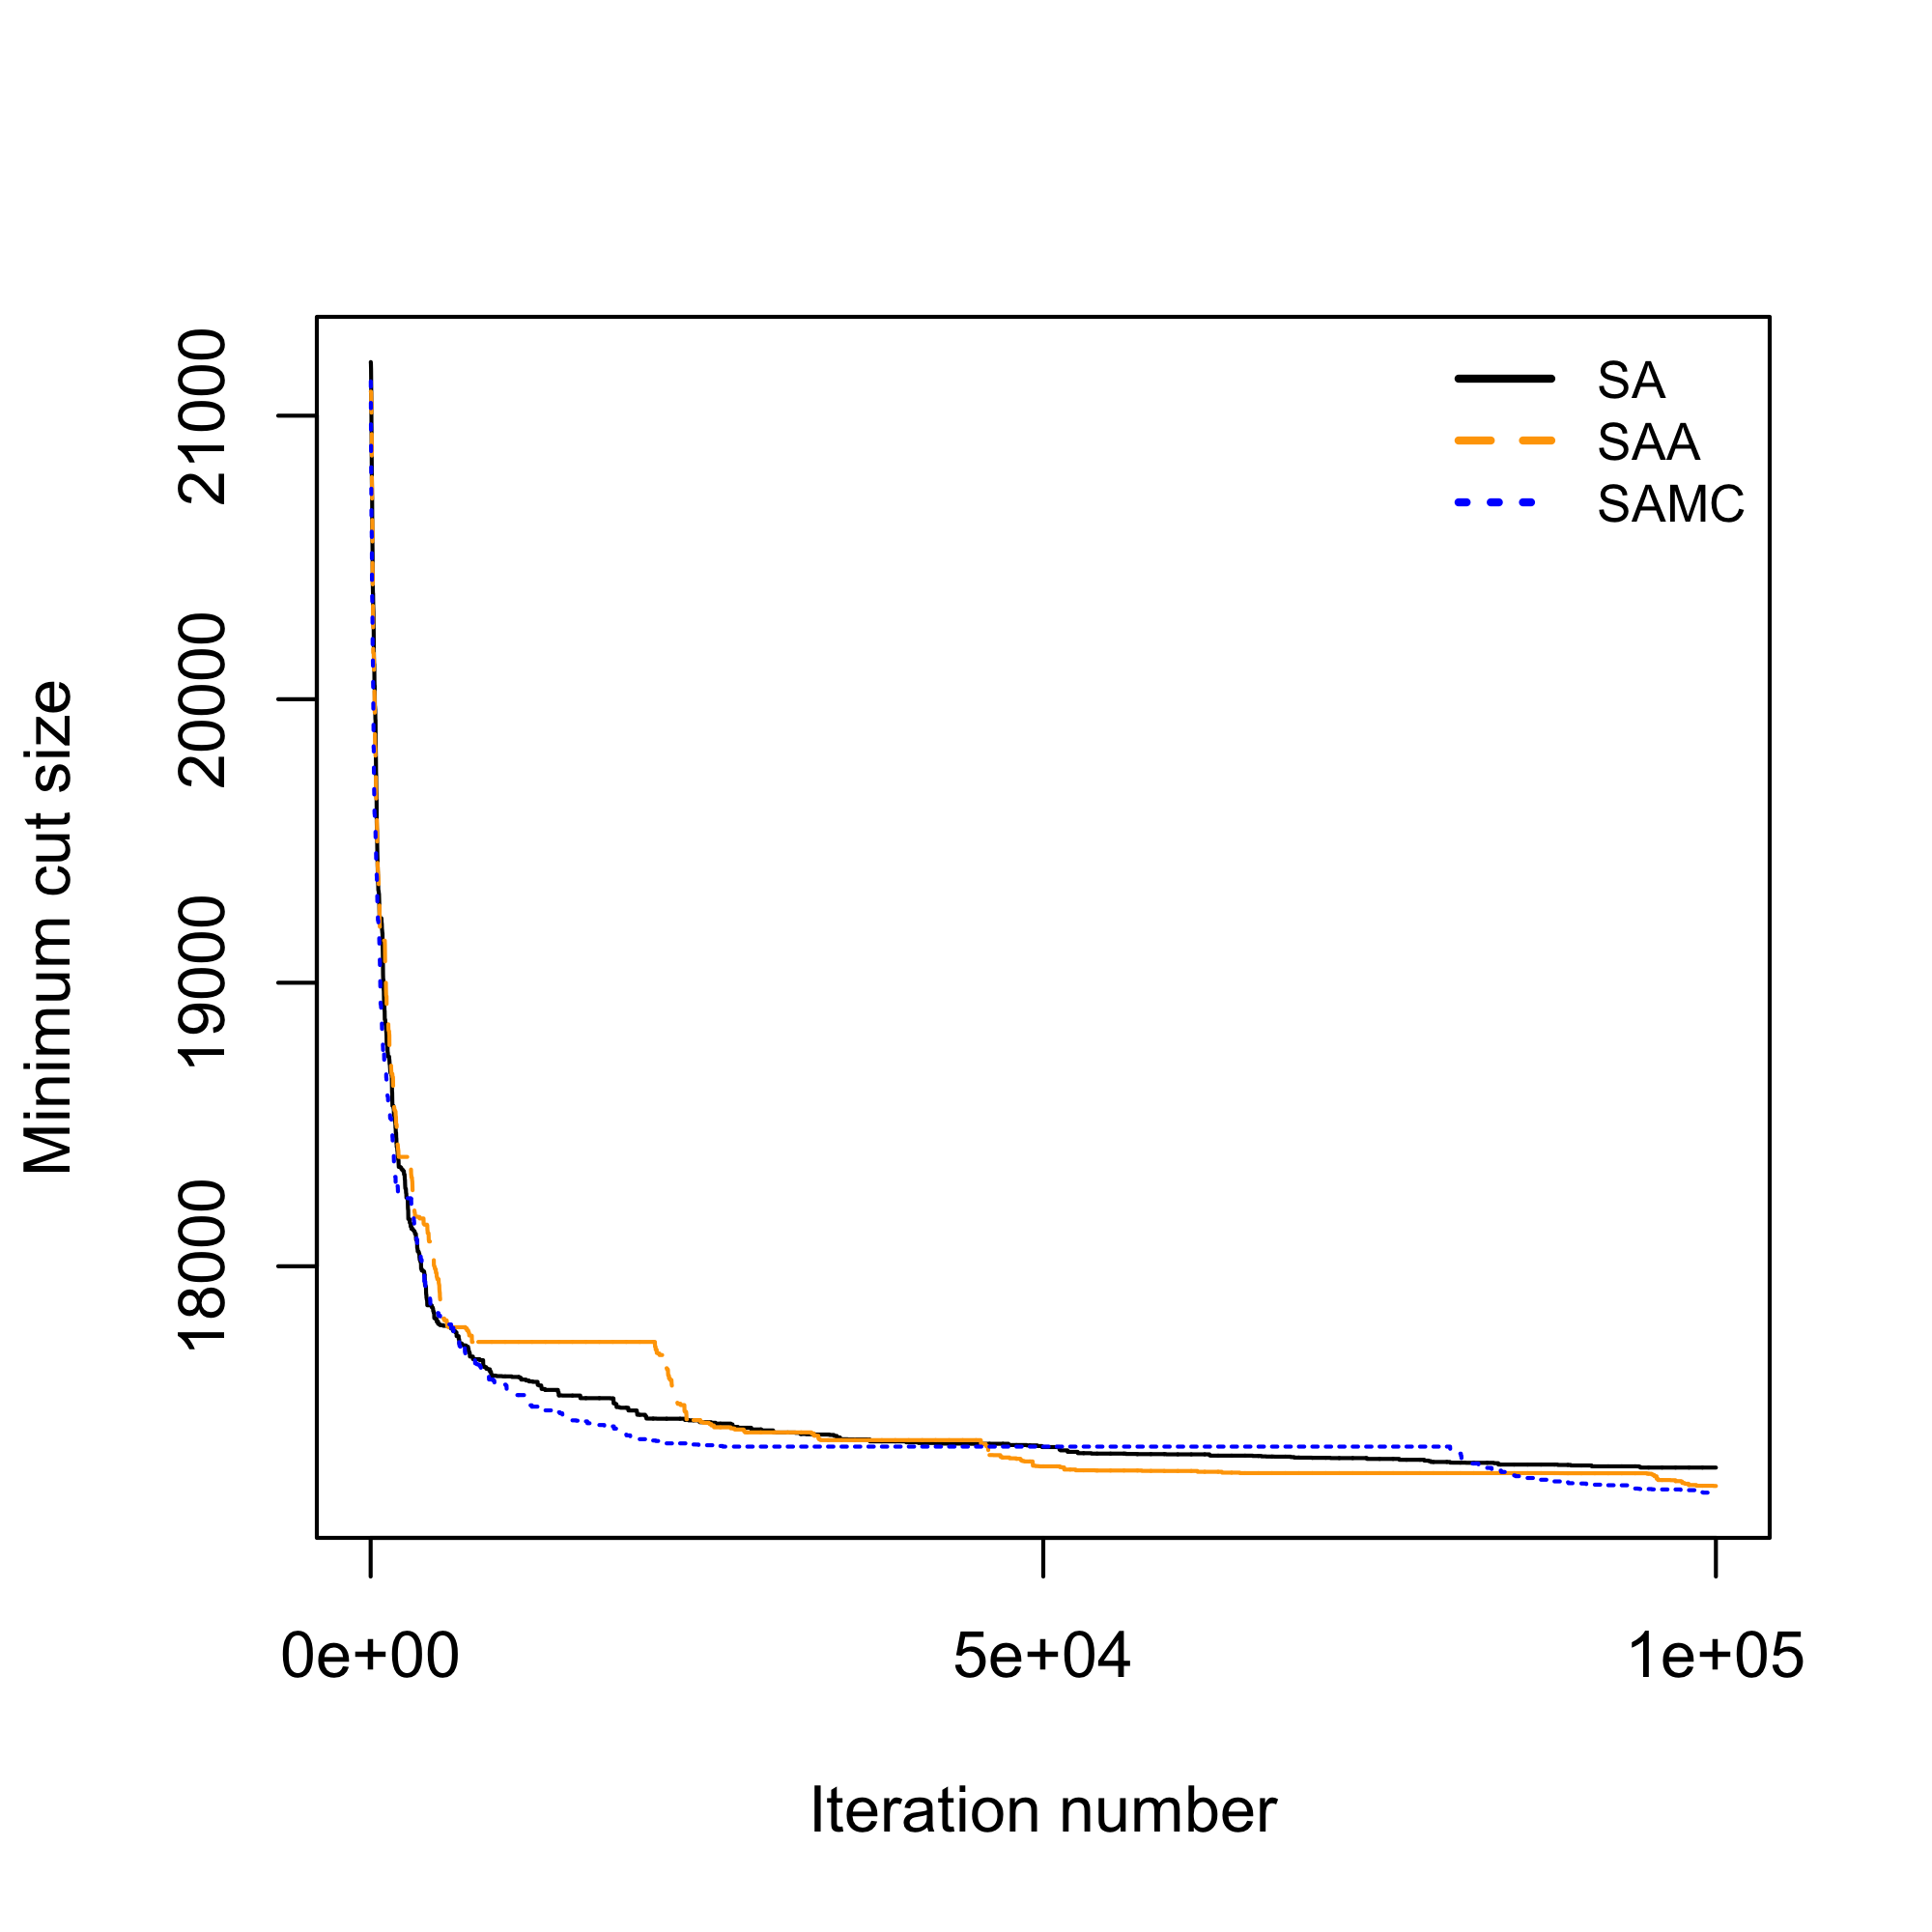
\includegraphics[width=.5\textwidth]{images/graph_min_cut_n750_iter1e+05}
  \end{tabular}
  \caption{Comparison of SA, SAA, and SAMC for $n = 750$}
  \label{fig:n750}
\end{figure}

\begin{figure}[hbpt]
  \begin{tabular}{cc}
    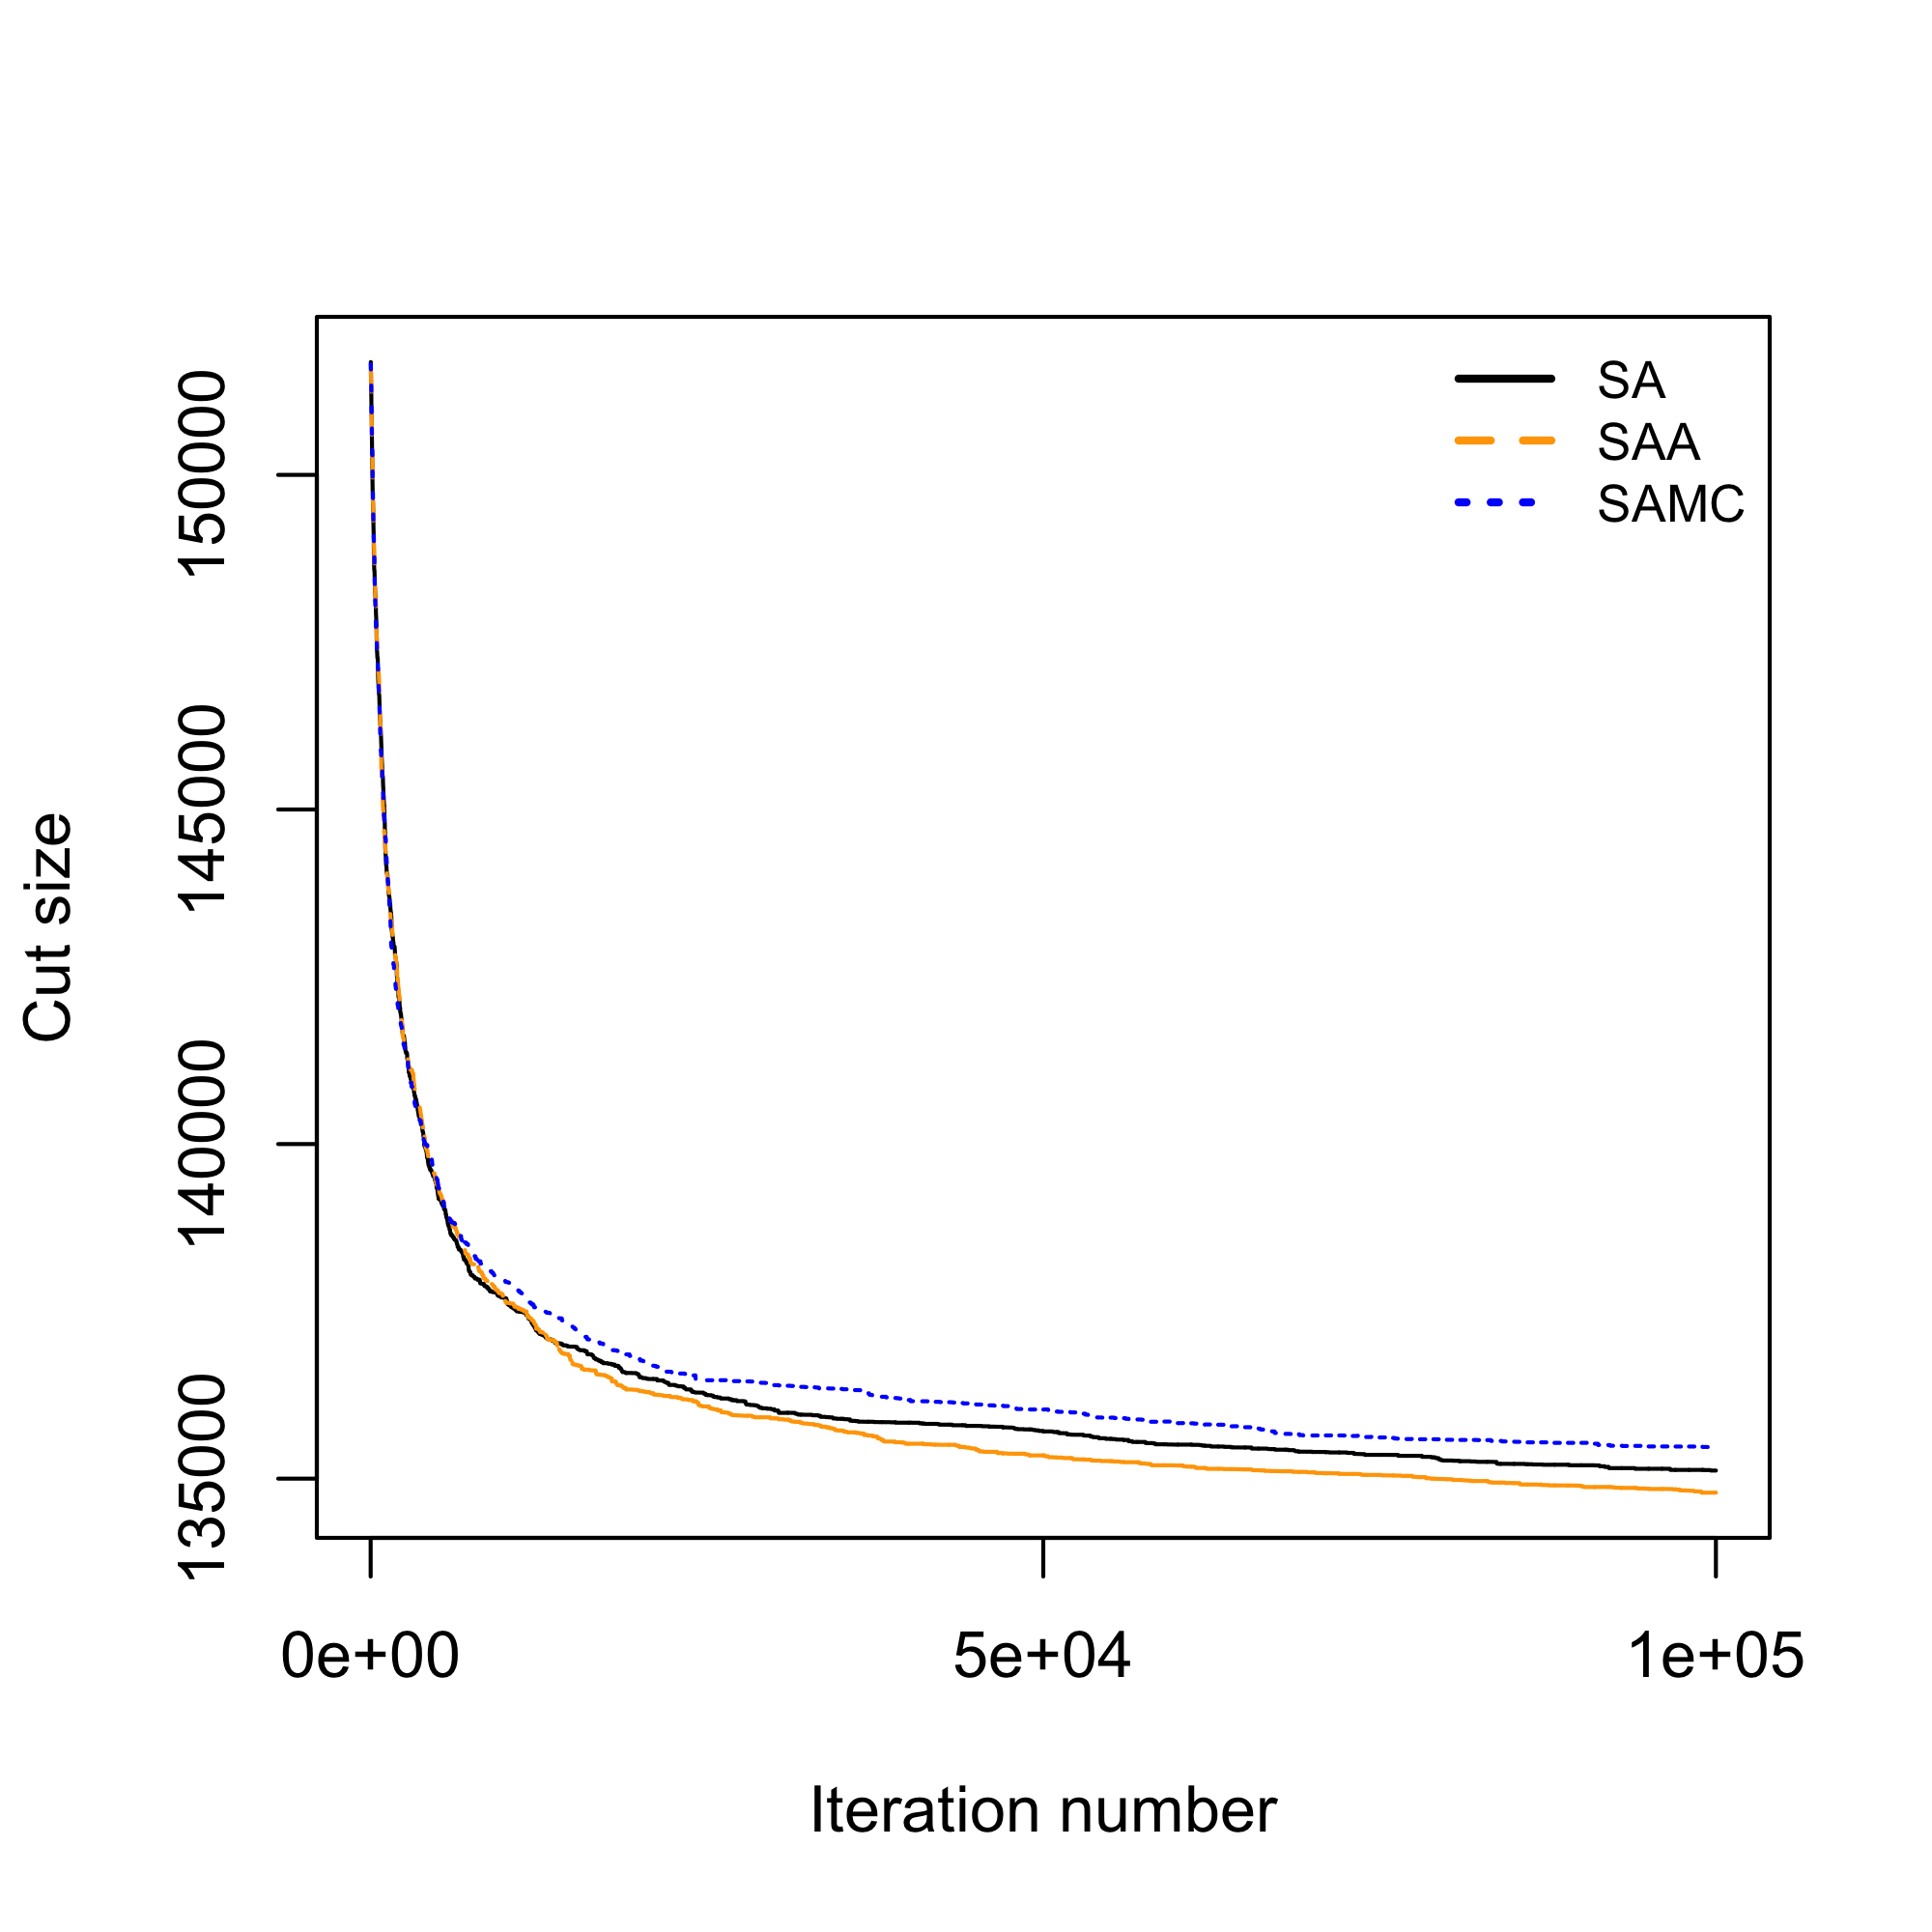
\includegraphics[width=.5\textwidth]{images/graph_cut_n2000_iter1e+05}
    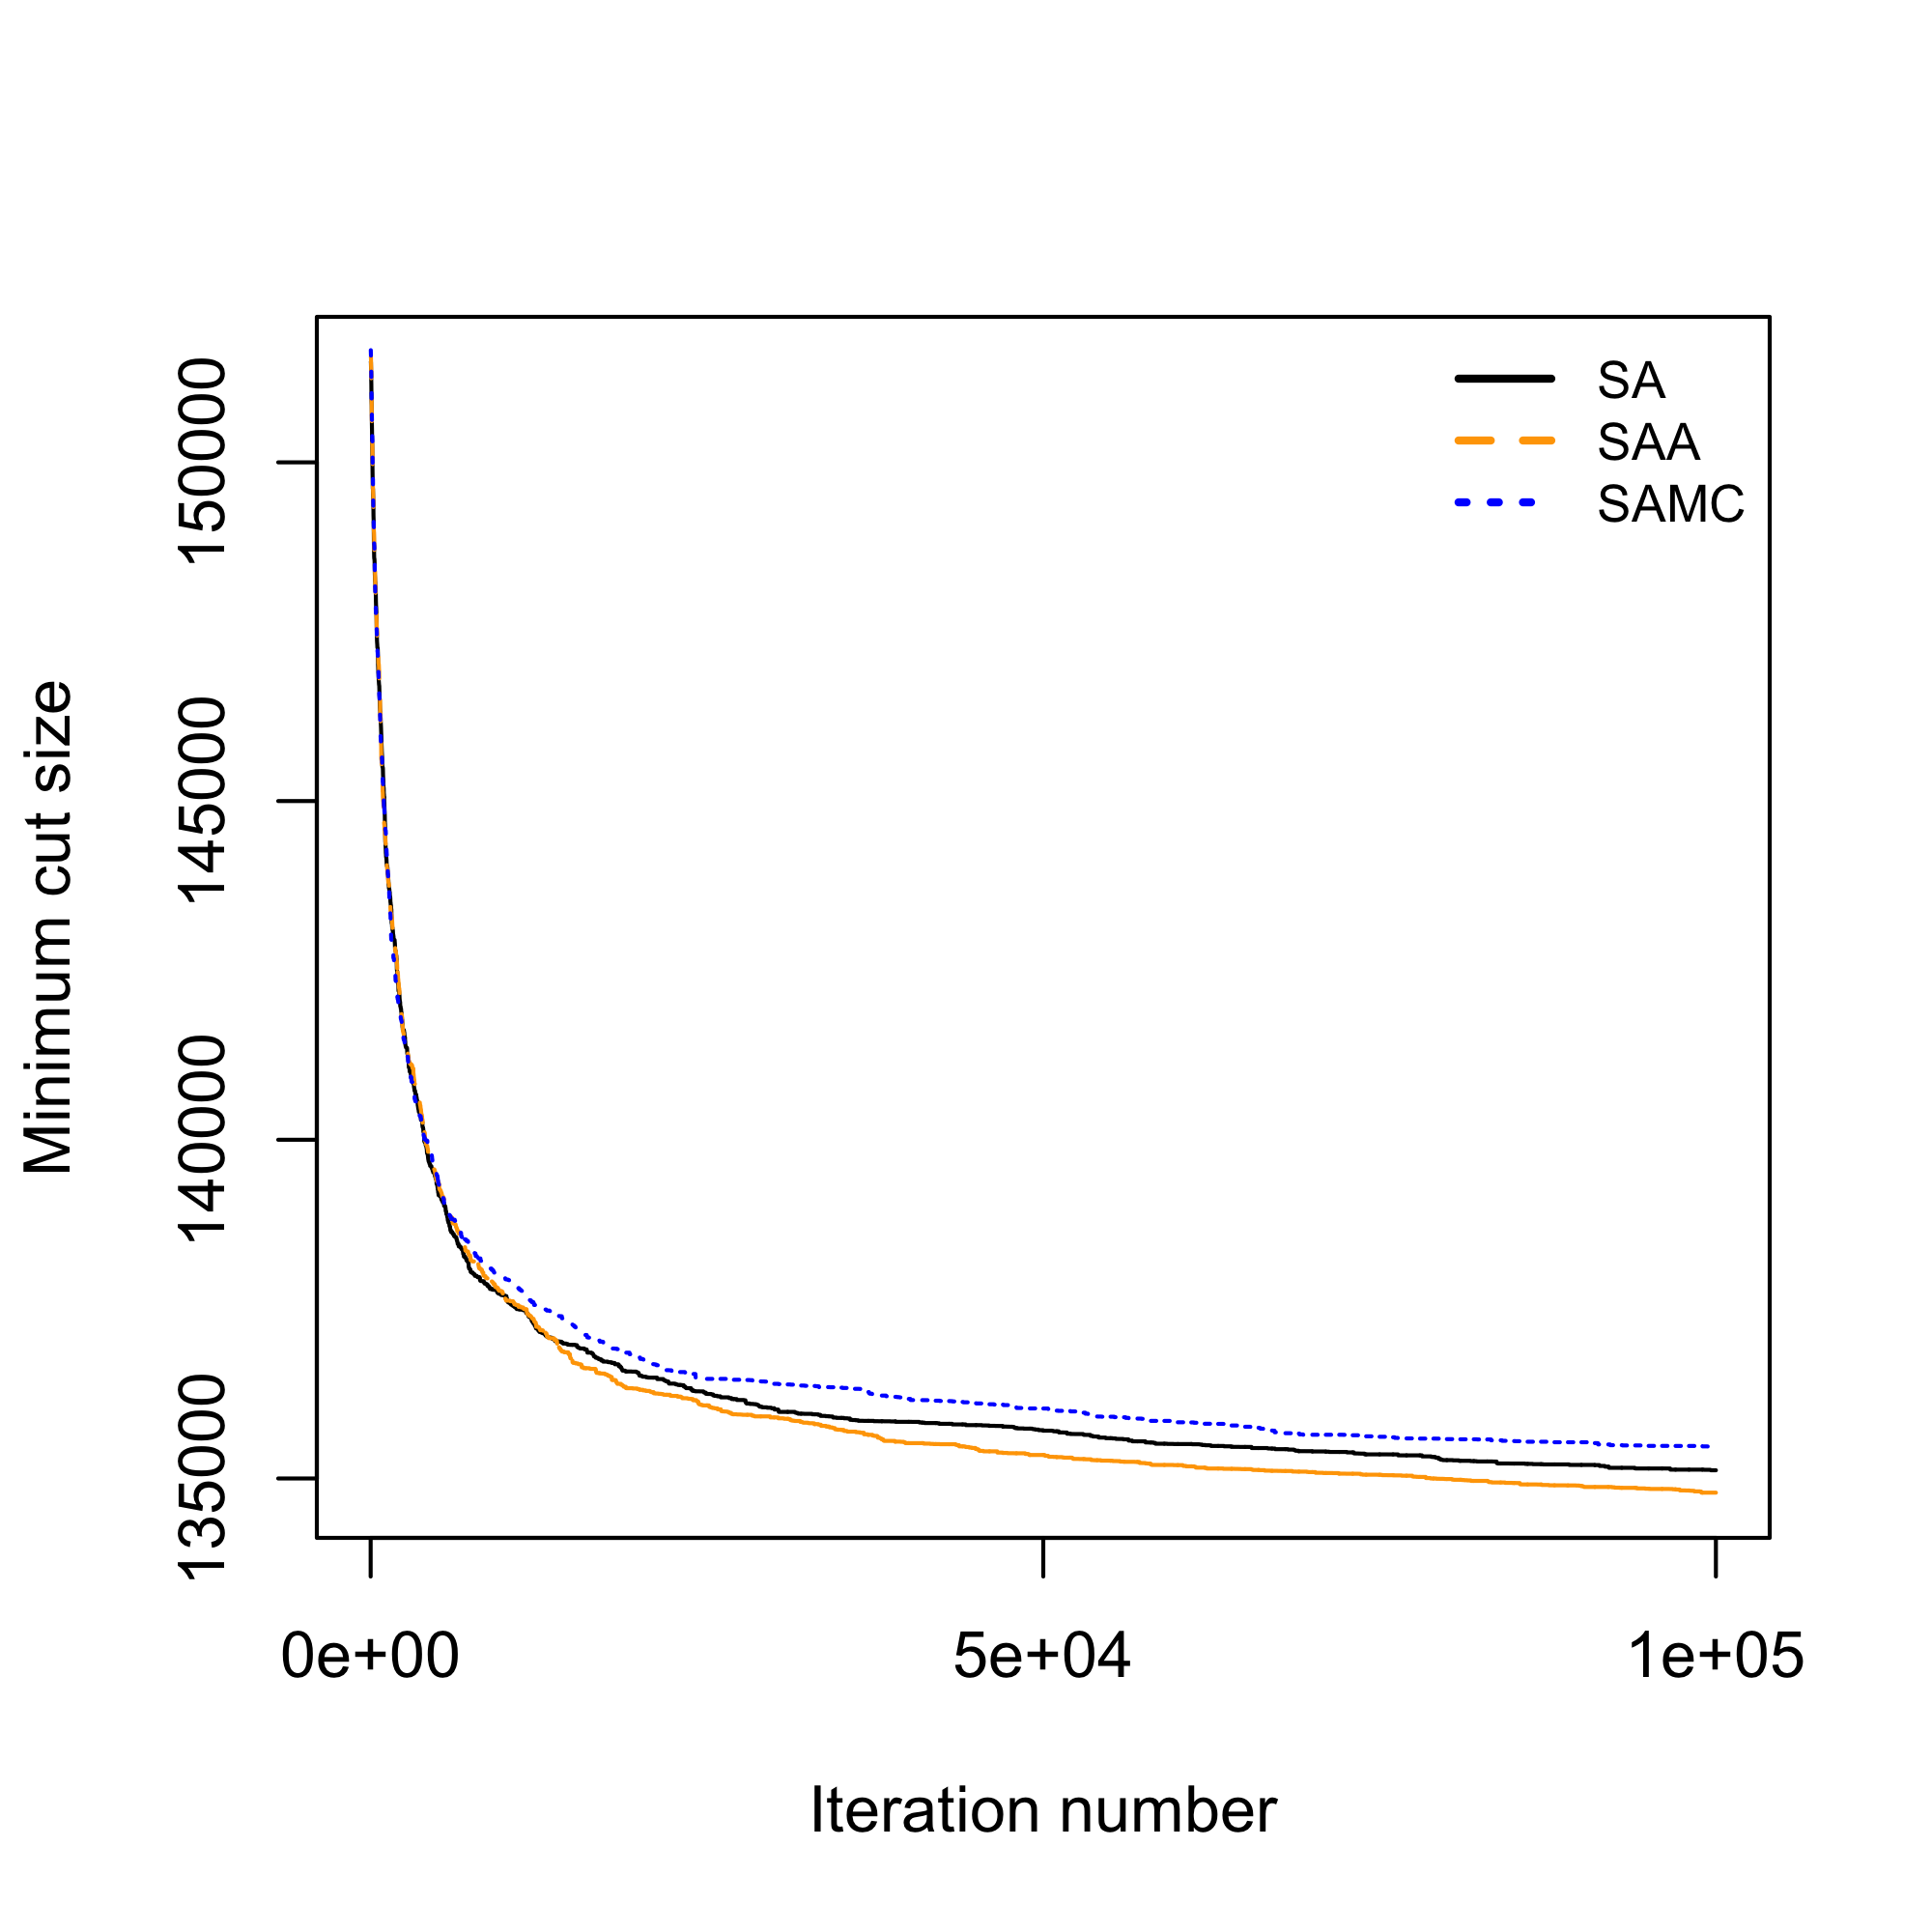
\includegraphics[width=.5\textwidth]{images/graph_min_cut_n2000_iter1e+05}
  \end{tabular}
  \caption{Comparison of SA, SAA, and SAMC for $n = 2000$}
  \label{fig:n2000}
\end{figure}

\begin{figure}[hbpt]
  \begin{tabular}{cc}
    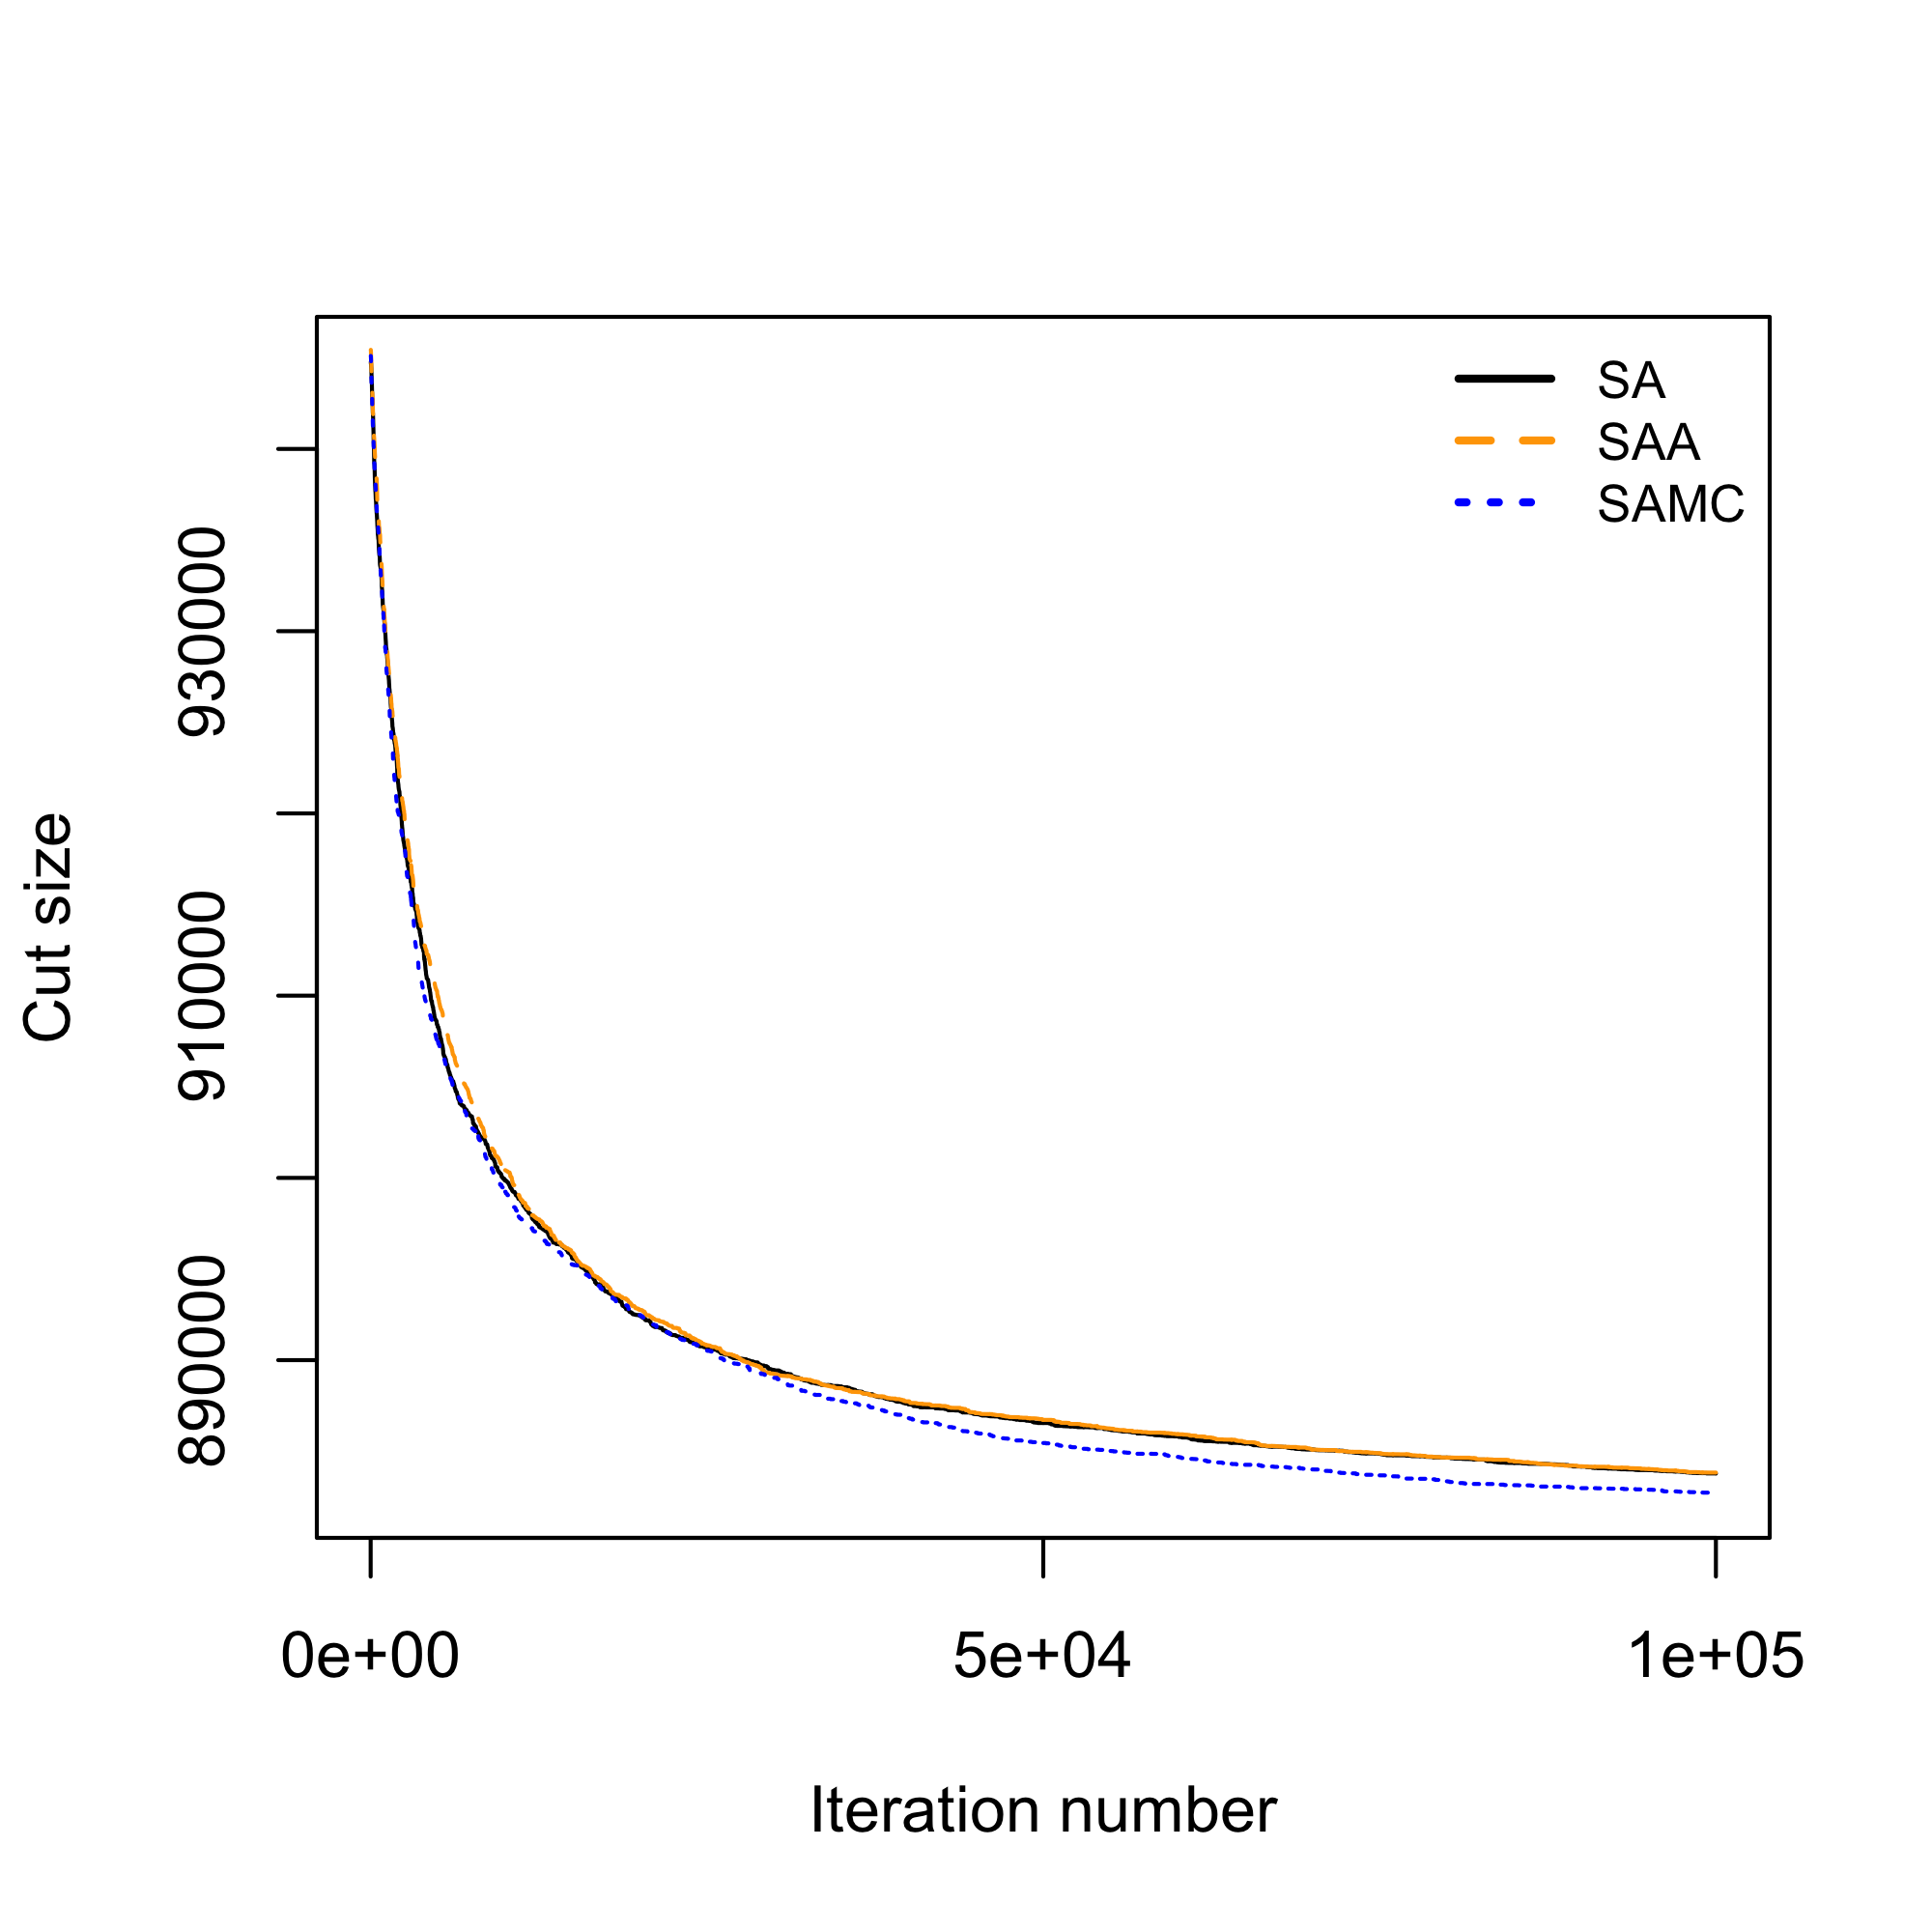
\includegraphics[width=.5\textwidth]{images/graph_cut_n5000_iter1e+05}
    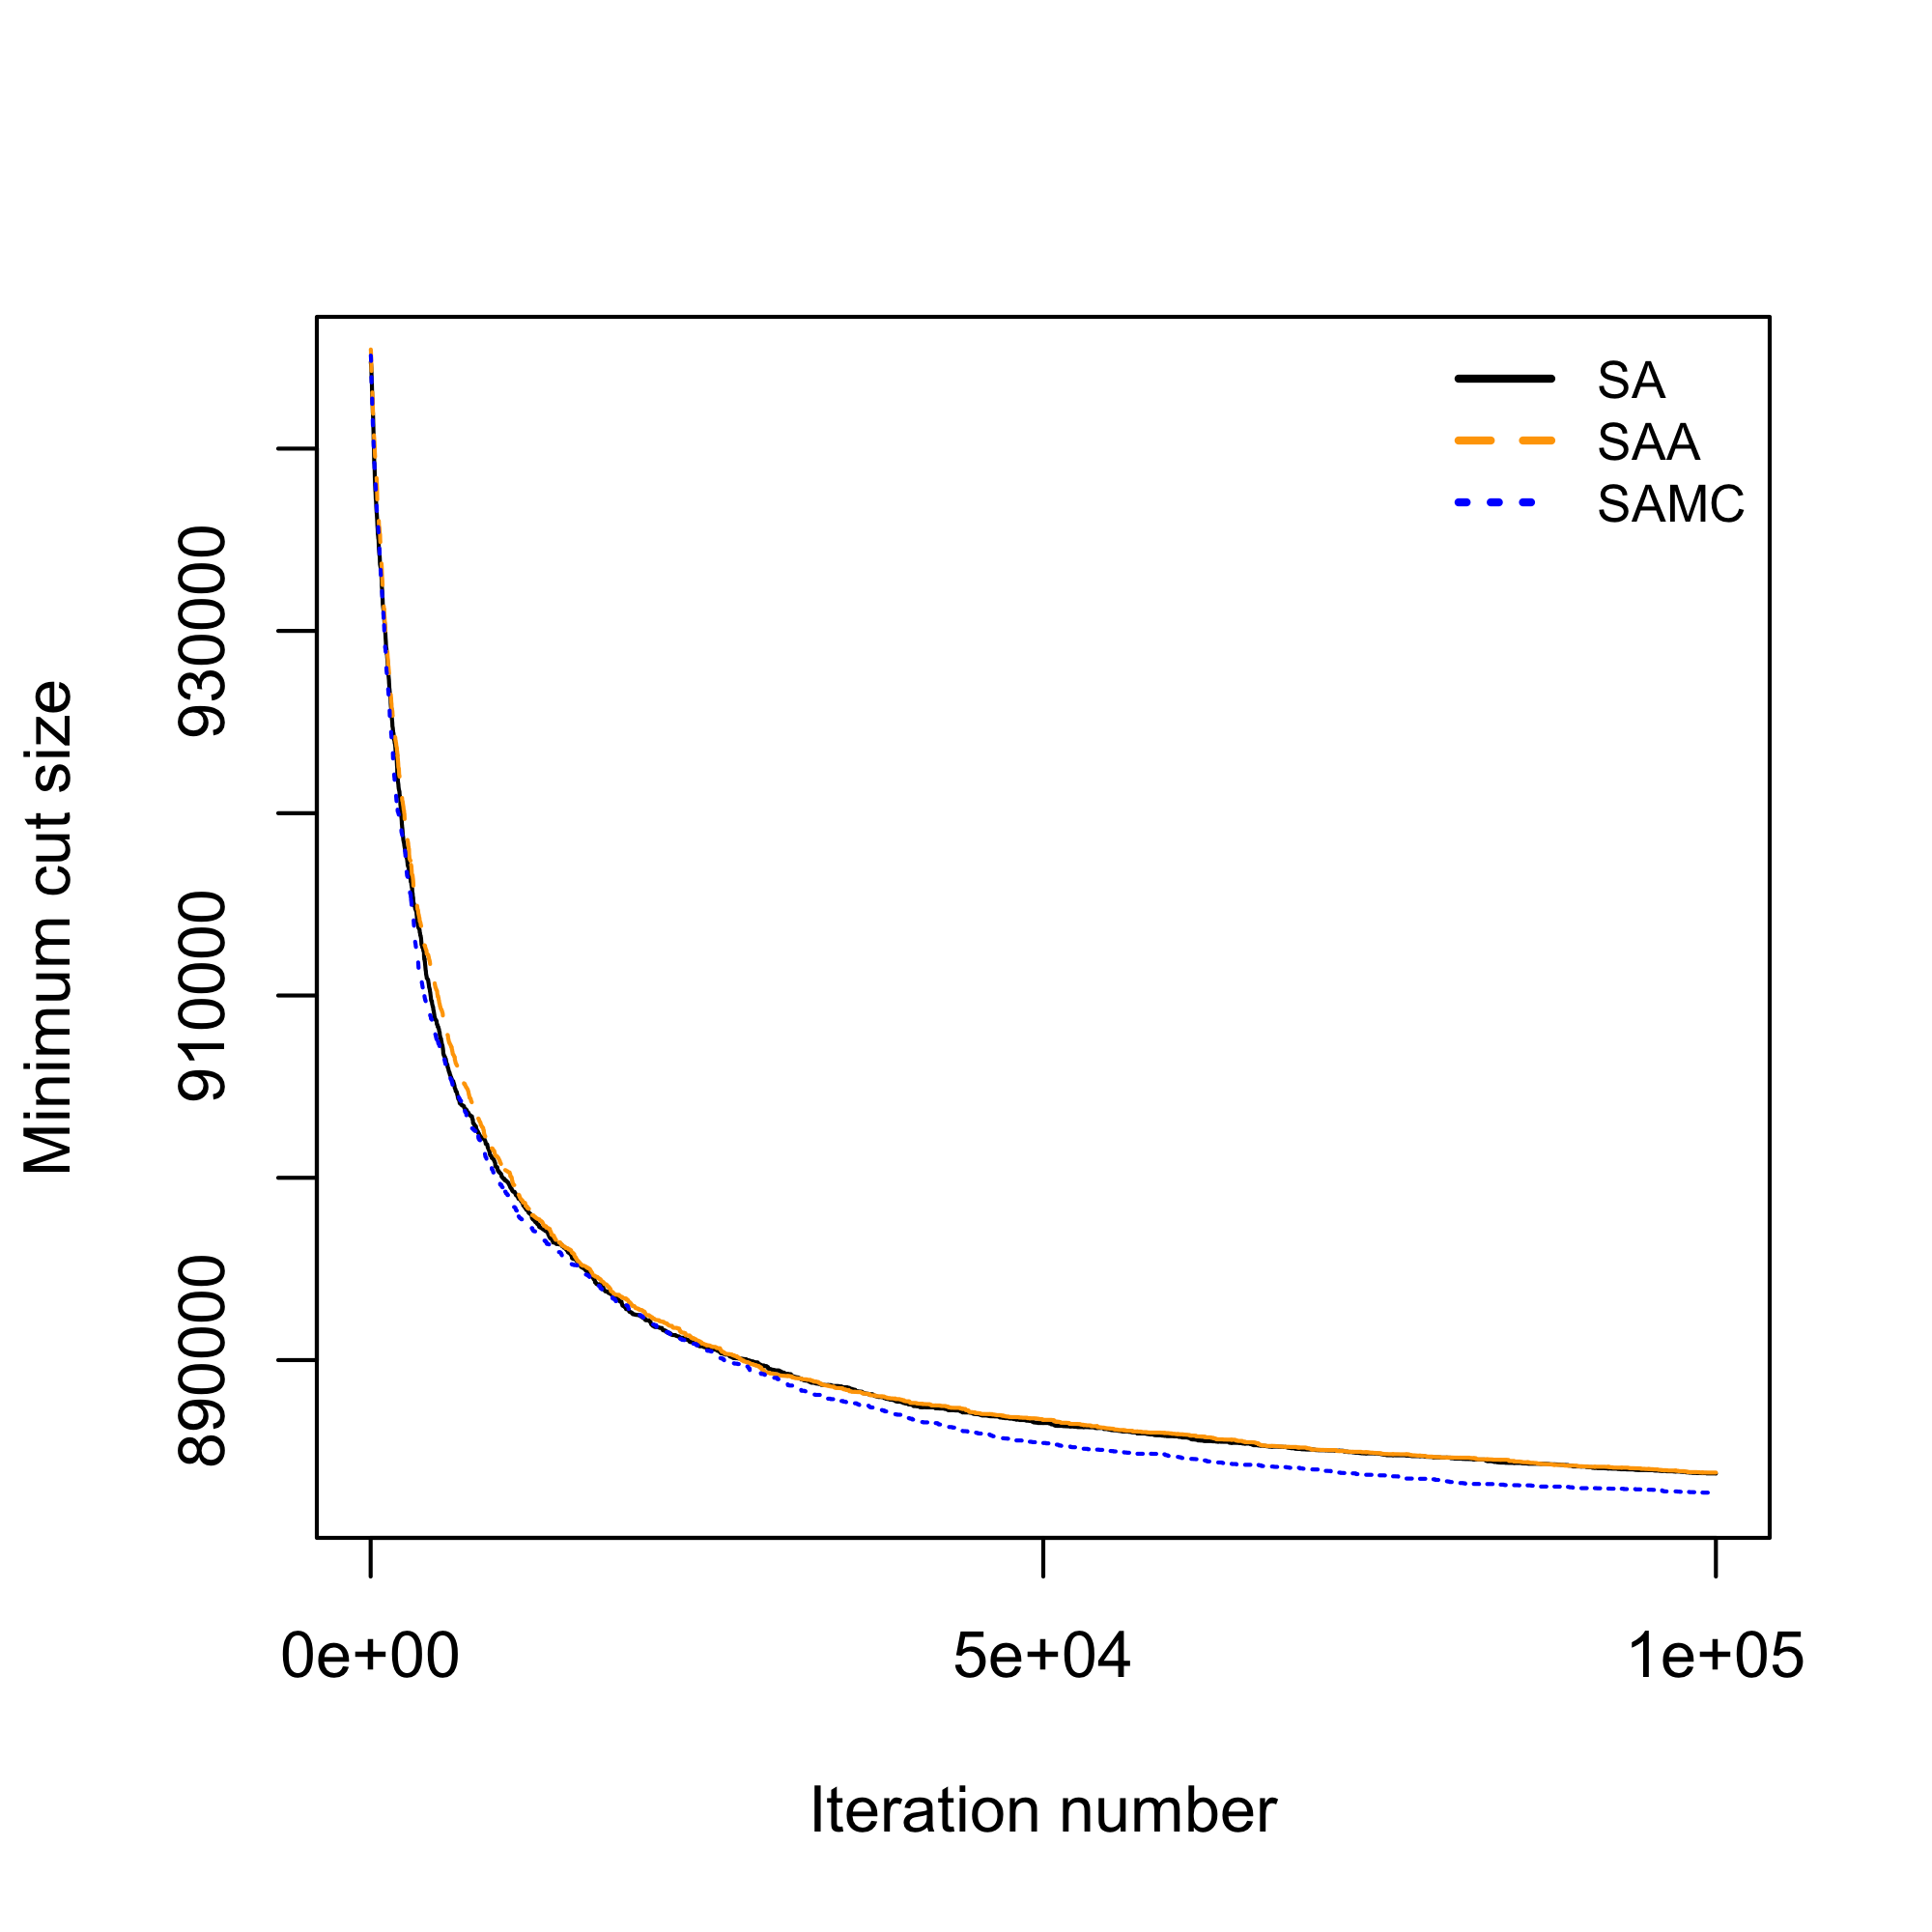
\includegraphics[width=.5\textwidth]{images/graph_min_cut_n5000_iter1e+05}
  \end{tabular}
  \caption{Comparison of SA, SAA, and SAMC for $n = 5000$}
  \label{fig:n5000}
\end{figure}

\begin{figure}[hbpt]
  \centering
  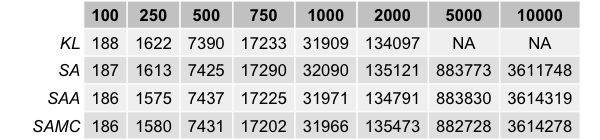
\includegraphics[width=.9\textwidth]{images/graph_all_vals_iter1e+05}
  \caption{Minimum cut found by each procedure for graph size $n$.}
  \label{fig:allvals}
\end{figure}

\begin{figure}[hbpt]
  \centering
  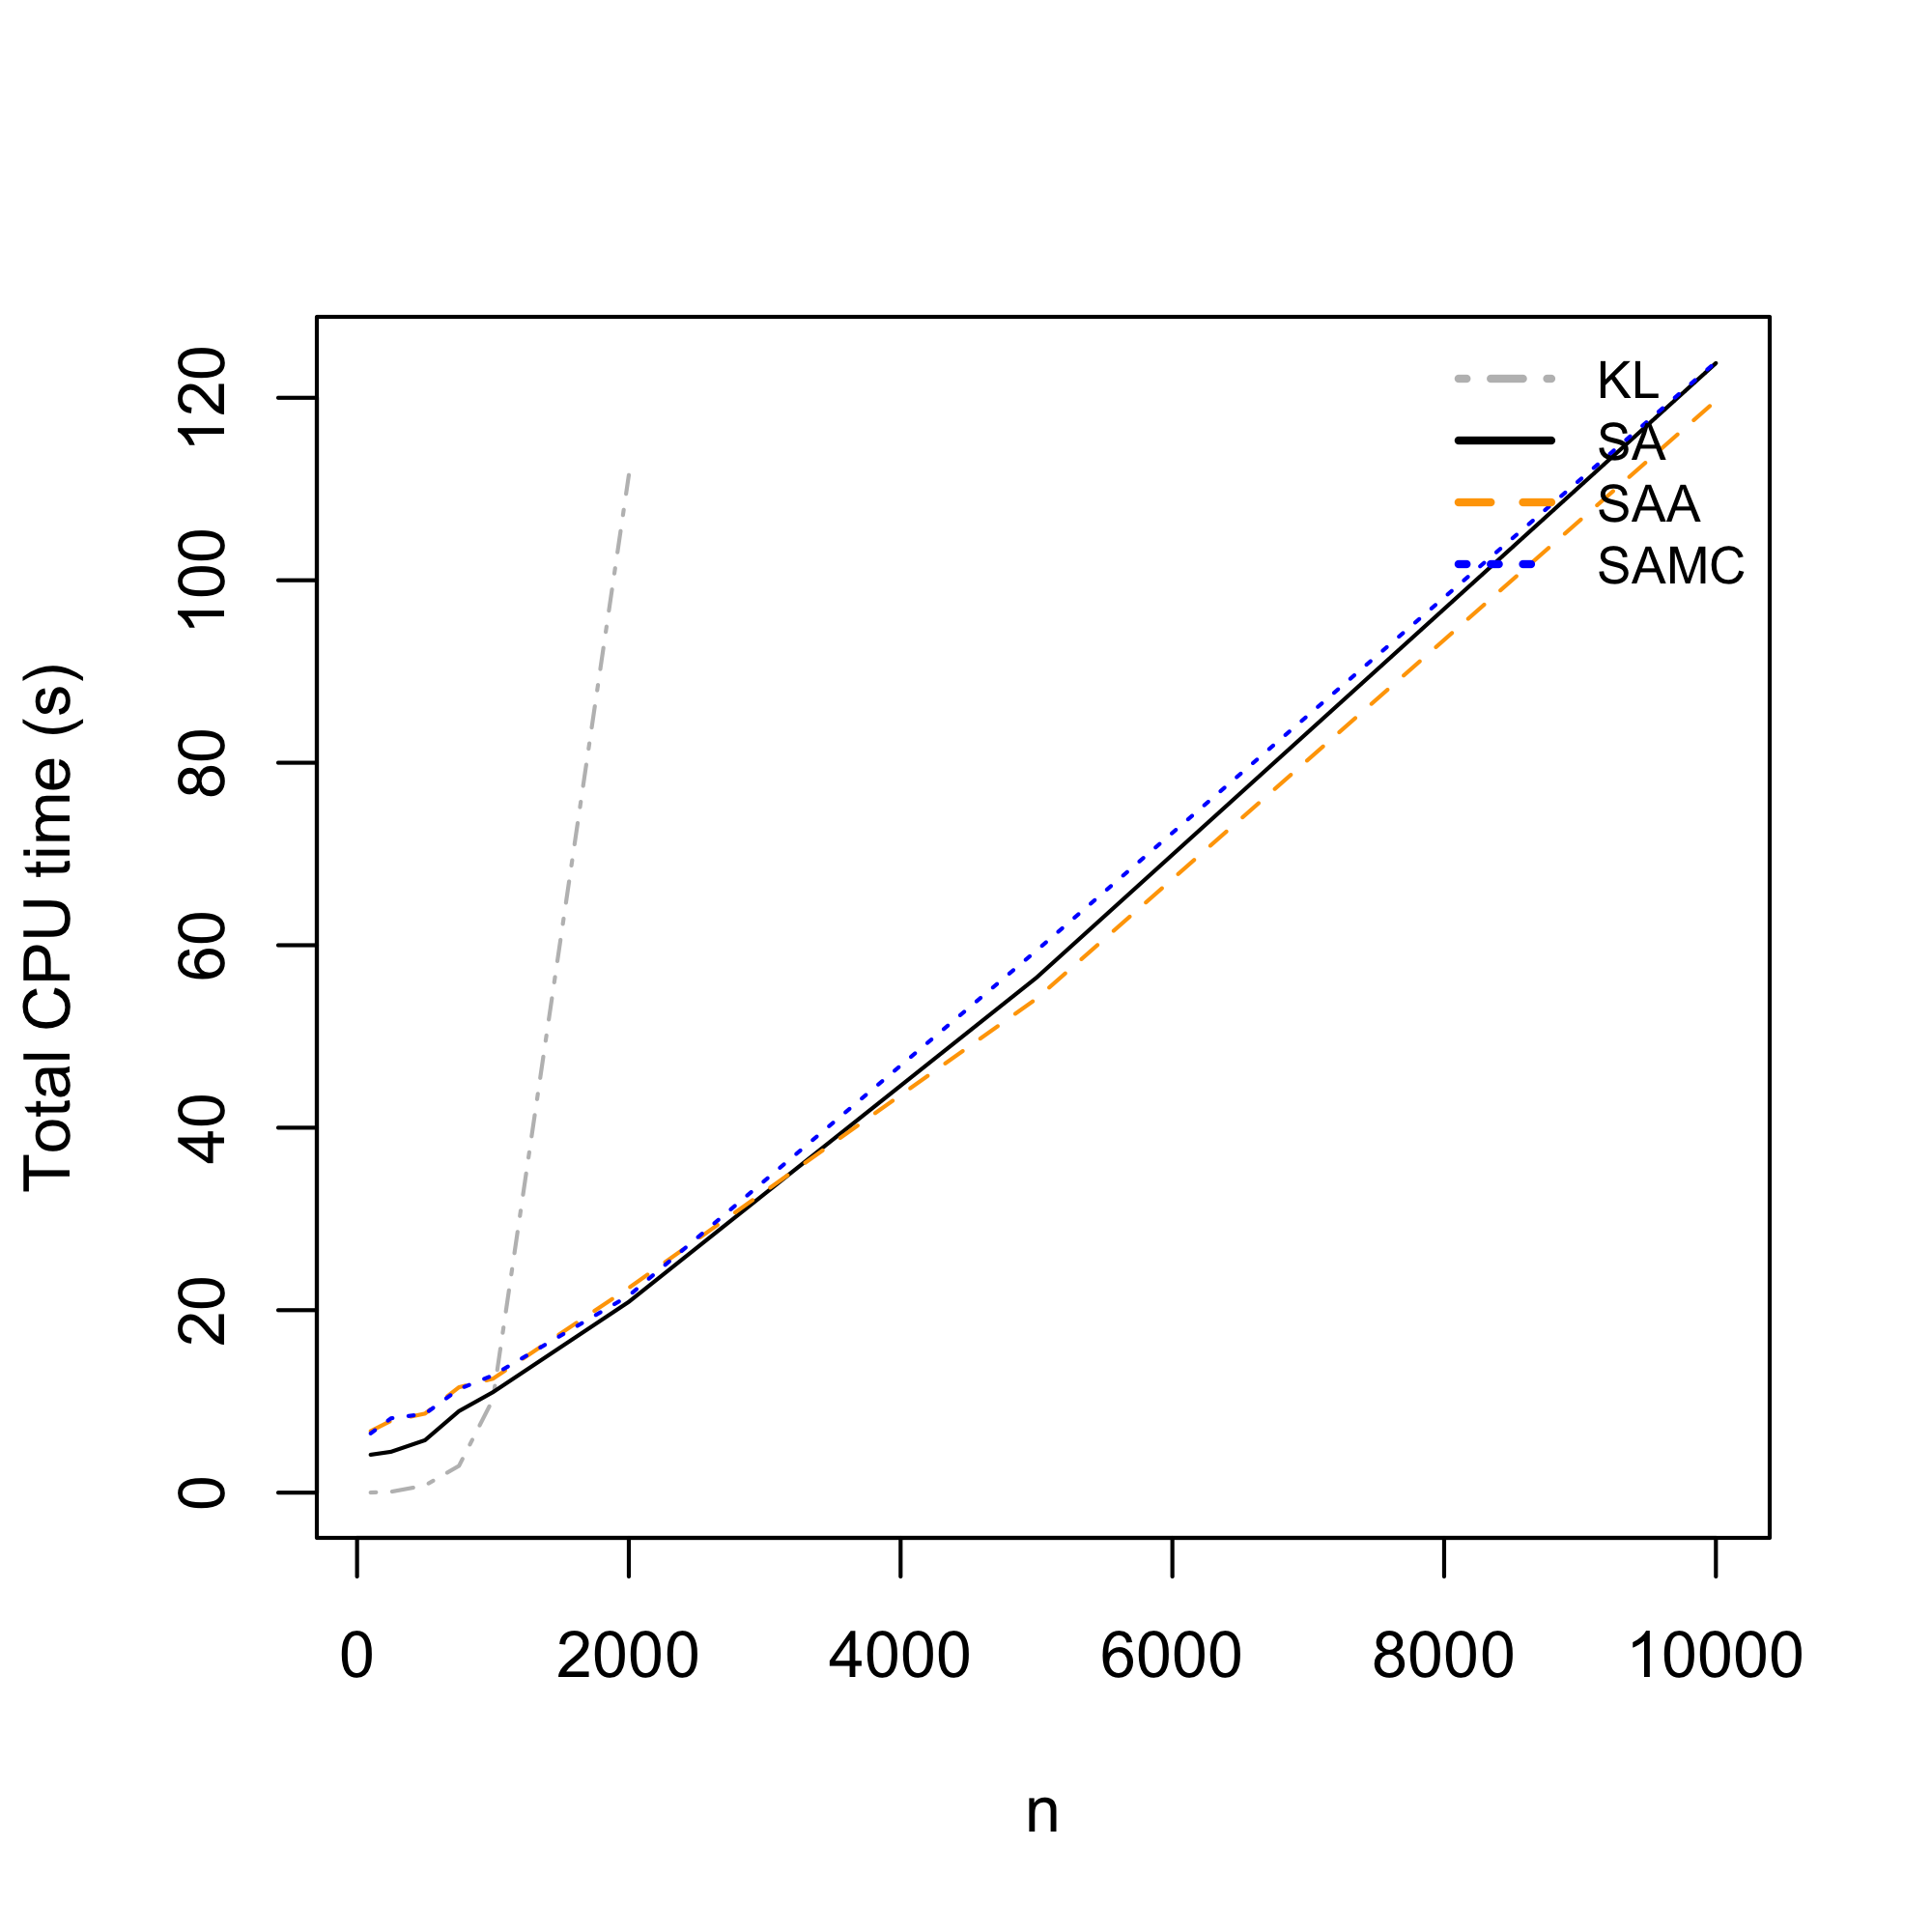
\includegraphics[width=.65\textwidth]{images/graph_all_times_iter1e+05}
  \caption{Total CPU time for graph size $n$. The KL algorithm was not run for $n > 2000$.}
  \label{fig:alltimes}
\end{figure}

\section{Discussion}\label{discussion}

For graphs with \(1000\) or fewer verticies, the KL algorithm is a very
good heuristic to use; it is fast and often produces the best partition.
However, because of its \(O(n^3)\) complexity, KL slows down
dramatically for graphs of size \(2000\) or larger. On the otherhand,
the stochastic algorithms run in linear time and can easily handle
larger graphs. The SAA and SAMC procedures have extra bookkeeping due to
the partitioning of the sample space, so they tend to run slightly
longer than SA. However, they also tend to find a minimum cut faster
than SA. Regardless, more simulations are required before we can
accurately compare SA, SAA, and SAMC.

The key property of SAMC is its ability to freely move around the sample
space. This property is observed in figure \ref{fig:n100} and figure
\ref{fig:n250}. Both SAA and SAMC explore the sample space much more
than SA, which allows them to not only avoid local traps but also find
optimal points quickly. As the graph size increases they tend to explore
less, but this may be due to the way the partition was chosen.
Alternatively, since the minimum cut size increase with graph size,
perhaps a rescaling of the edge weights could lead to better results.
Either way, these results suggest that SAA and SAMC are likely
improvements over SA.

\section*{Appendix A: R code}\label{appendix-a-r-code}
\addcontentsline{toc}{section}{Appendix A: R code}

\begin{Shaded}
\begin{Highlighting}[]
\KeywordTok{set.seed}\NormalTok{(}\DecValTok{1000}\NormalTok{)}
\KeywordTok{library}\NormalTok{(gridExtra)}

\CommentTok{# #####################################################}
\CommentTok{#}
\CommentTok{# Auxillary functions.}
\CommentTok{#}
\CommentTok{# #####################################################}
\CommentTok{#Generate data set for t-test.}
\NormalTok{generate_data <-}\StringTok{ }\NormalTok{function(}\DataTypeTok{n =} \DecValTok{100}\NormalTok{, }\DataTypeTok{weights =} \DecValTok{2}\NormalTok{) \{}
  \NormalTok{W <-}\StringTok{ }\KeywordTok{matrix}\NormalTok{(}\DecValTok{0}\NormalTok{, }\DataTypeTok{nrow =} \NormalTok{n, }\DataTypeTok{ncol =} \NormalTok{n)}
    \NormalTok{for(i in }\DecValTok{1}\NormalTok{:n) \{}
      \NormalTok{m <-}\StringTok{ }\KeywordTok{rbinom}\NormalTok{(}\DecValTok{1}\NormalTok{, n, }\FloatTok{0.05}\NormalTok{) }\CommentTok{#Number of latent variables.}
      \NormalTok{latent_vars <-}\StringTok{ }\KeywordTok{sample}\NormalTok{((}\DecValTok{1}\NormalTok{:n)[-i], m)}
      \NormalTok{vals <-}\StringTok{ }\KeywordTok{runif}\NormalTok{(m)*weights}
      \NormalTok{W[i, latent_vars] <-}\StringTok{ }\NormalTok{W[i, latent_vars] +}\StringTok{ }\NormalTok{vals}
      \NormalTok{W[latent_vars, i] <-}\StringTok{ }\NormalTok{W[i, latent_vars] +}\StringTok{ }\NormalTok{vals}
    \NormalTok{\}}
\NormalTok{\}}

\CommentTok{# W: 2n by 2n adjacency matrix}
\CommentTok{# A: vector of size n containing the indicies in one subset.}
\CommentTok{# a: include if cost of only one node is desired.}
\NormalTok{external_cost <-}\StringTok{ }\NormalTok{function(W, A, }\DataTypeTok{a =} \OtherTok{NULL}\NormalTok{) \{}
  \NormalTok{if(!}\KeywordTok{is.null}\NormalTok{(a)) \{}
    \KeywordTok{return}\NormalTok{(}\KeywordTok{sum}\NormalTok{(W[a, -A]))}
  \NormalTok{\}}
  \NormalTok{c <-}\StringTok{ }\KeywordTok{rep}\NormalTok{(}\DecValTok{0}\NormalTok{, }\KeywordTok{nrow}\NormalTok{(W))}
  \NormalTok{c[A] <-}\StringTok{ }\KeywordTok{apply}\NormalTok{(W[A, -A], }\DecValTok{1}\NormalTok{, sum)}
  \NormalTok{c[-A] <-}\StringTok{ }\KeywordTok{apply}\NormalTok{(W[-A, A], }\DecValTok{1}\NormalTok{, sum)}
  \KeywordTok{return}\NormalTok{(c)}
\NormalTok{\}}

\CommentTok{# W: 2n by 2n adjacency matrix}
\CommentTok{# A: vector of size n containing the indicies in one subset.}
\CommentTok{# a: include if cost of only one node is desired.}
\NormalTok{internal_cost <-}\StringTok{ }\NormalTok{function(W, A, }\DataTypeTok{a =} \OtherTok{NULL}\NormalTok{) \{}
  \NormalTok{if(!}\KeywordTok{is.null}\NormalTok{(a)) \{}
    \KeywordTok{return}\NormalTok{(}\KeywordTok{sum}\NormalTok{(W[a, A]))}
  \NormalTok{\}}
  \NormalTok{c <-}\StringTok{ }\KeywordTok{rep}\NormalTok{(}\DecValTok{0}\NormalTok{, }\KeywordTok{nrow}\NormalTok{(W))}
  \NormalTok{c[A] <-}\StringTok{ }\KeywordTok{apply}\NormalTok{(W[A, A], }\DecValTok{1}\NormalTok{, sum)}
  \NormalTok{c[-A] <-}\StringTok{ }\KeywordTok{apply}\NormalTok{(W[-A, -A], }\DecValTok{1}\NormalTok{, sum)}
  \KeywordTok{return}\NormalTok{(c)}
\NormalTok{\}}

\CommentTok{#Swap two nodes between partitions A and -A.}
\NormalTok{move <-}\StringTok{ }\NormalTok{function(W, A) \{}
  \NormalTok{B <-}\StringTok{ }\NormalTok{(}\DecValTok{1}\NormalTok{:(}\DecValTok{2}\NormalTok{*}\KeywordTok{length}\NormalTok{(A)))[-A]}
  \NormalTok{a <-}\StringTok{ }\KeywordTok{sample}\NormalTok{(A, }\DecValTok{1}\NormalTok{)}
  \NormalTok{b <-}\StringTok{ }\KeywordTok{sample}\NormalTok{(B, }\DecValTok{1}\NormalTok{)}
  \NormalTok{delta_t <-}\StringTok{ }\KeywordTok{internal_cost}\NormalTok{(W, A, a) +}\StringTok{ }
\StringTok{    }\KeywordTok{internal_cost}\NormalTok{(W, B, b) -}\StringTok{ }\KeywordTok{external_cost}\NormalTok{(W, A, a) -}\StringTok{ }
\StringTok{    }\KeywordTok{external_cost}\NormalTok{(W, B, b) +}\StringTok{ }\DecValTok{2}\NormalTok{*W[a, b]}
  \NormalTok{A_new <-}\StringTok{ }\NormalTok{A}
  \NormalTok{A_new[}\KeywordTok{which}\NormalTok{(A ==}\StringTok{ }\NormalTok{a)] <-}\StringTok{ }\NormalTok{b}
  \KeywordTok{return}\NormalTok{(}\KeywordTok{list}\NormalTok{(}\DataTypeTok{A_new =} \NormalTok{A_new, }\DataTypeTok{delta_t =} \NormalTok{delta_t))}
\NormalTok{\}}

\NormalTok{cut_size <-}\StringTok{ }\NormalTok{function(W, A) \{}
  \NormalTok{if(}\KeywordTok{length}\NormalTok{(}\KeywordTok{unique}\NormalTok{(A)) !=}\StringTok{ }\KeywordTok{length}\NormalTok{(A)) \{}
    \KeywordTok{stop}\NormalTok{(}\StringTok{"A should contain unique elements."}\NormalTok{)}
  \NormalTok{\}}
  \KeywordTok{return}\NormalTok{(}\KeywordTok{sum}\NormalTok{(}\KeywordTok{external_cost}\NormalTok{(W, A)[A]))}
\NormalTok{\}}

\CommentTok{#Find which subset t belongs to in the partition.}
\NormalTok{get_partition_index<-function(t, E)\{}
  \NormalTok{m <-}\StringTok{ }\KeywordTok{length}\NormalTok{(E)}
  \CommentTok{#First check edge cases.}
  \NormalTok{if(t <}\StringTok{ }\NormalTok{E[}\DecValTok{1}\NormalTok{]) \{}
    \KeywordTok{return}\NormalTok{(}\DecValTok{1}\NormalTok{)}
  \NormalTok{\} else if (t >=}\StringTok{ }\NormalTok{E[m]) \{}
    \KeywordTok{return}\NormalTok{(m +}\StringTok{ }\DecValTok{1}\NormalTok{)}
  \NormalTok{\} }
  
  \CommentTok{#Binary search to find which subset contains t.}
  \NormalTok{binary_search <-}\StringTok{ }\NormalTok{function(t, indicies) \{}
    \NormalTok{m <-}\StringTok{ }\KeywordTok{length}\NormalTok{(indicies)}
    \NormalTok{if(m ==}\StringTok{ }\DecValTok{1}\NormalTok{) \{}
      \NormalTok{if(t <}\StringTok{ }\NormalTok{E[indicies]) \{}
        \KeywordTok{return}\NormalTok{(indicies)}
      \NormalTok{\} else \{}
        \KeywordTok{return}\NormalTok{(indicies +}\StringTok{ }\DecValTok{1}\NormalTok{)}
      \NormalTok{\}}
    \NormalTok{\}}
    \NormalTok{i <-}\StringTok{ }\KeywordTok{ceiling}\NormalTok{(m/}\DecValTok{2}\NormalTok{) +}\StringTok{ }\DecValTok{1} \CommentTok{#Start in the middle.}
    \NormalTok{if(t >=}\StringTok{ }\NormalTok{E[indicies[i -}\StringTok{ }\DecValTok{1}\NormalTok{]] &&}\StringTok{ }\NormalTok{t <}\StringTok{ }\NormalTok{E[indicies[i]]) \{}
      \KeywordTok{return}\NormalTok{(indicies[i])}
    \NormalTok{\}}
    \NormalTok{if(t <}\StringTok{ }\NormalTok{E[indicies[i -}\StringTok{ }\DecValTok{1}\NormalTok{]]) \{}
      \KeywordTok{return}\NormalTok{(}\KeywordTok{binary_search}\NormalTok{(t, indicies[}\DecValTok{1}\NormalTok{:(i -}\StringTok{ }\DecValTok{1}\NormalTok{)]))}
    \NormalTok{\} else \{}
      \KeywordTok{return}\NormalTok{(}\KeywordTok{binary_search}\NormalTok{(t, indicies[i:m]))}
    \NormalTok{\}}
  \NormalTok{\}}
  
  \KeywordTok{return}\NormalTok{(}\KeywordTok{binary_search}\NormalTok{(t, }\DecValTok{2}\NormalTok{:m))}
\NormalTok{\}}



\NormalTok{## Approximate bisection}
\CommentTok{# Code adapted from C.Ladroue at }
\CommentTok{#  https://www.r-bloggers.com/graph-bisection-in-r/}
\CommentTok{# #####################################################}
\CommentTok{#}
\CommentTok{# KL}
\CommentTok{#}
\CommentTok{# #####################################################}
\NormalTok{KL <-}\StringTok{ }\NormalTok{function(W, }\DataTypeTok{A =} \OtherTok{NULL}\NormalTok{)\{}
  \NormalTok{n <-}\StringTok{ }\KeywordTok{nrow}\NormalTok{(W)}
  \NormalTok{m <-}\StringTok{ }\NormalTok{n/}\DecValTok{2}
  
  \CommentTok{# start off with a random partition}
  \NormalTok{if(}\KeywordTok{is.null}\NormalTok{(A)) \{}
    \NormalTok{A <-}\StringTok{ }\KeywordTok{sample}\NormalTok{(}\DecValTok{1}\NormalTok{:n, n/}\DecValTok{2}\NormalTok{, }\DataTypeTok{replace=}\OtherTok{FALSE}\NormalTok{)}
  \NormalTok{\}}
  \NormalTok{B <-}\StringTok{ }\NormalTok{(}\DecValTok{1}\NormalTok{:n)[-A]}
  
  \NormalTok{DA <-}\StringTok{ }\KeywordTok{rowSums}\NormalTok{(W[A, B]) -}\StringTok{ }\KeywordTok{rowSums}\NormalTok{(W[A, A]) +}\StringTok{ }\KeywordTok{diag}\NormalTok{(W[A, A])}
  \NormalTok{DB <-}\StringTok{ }\KeywordTok{rowSums}\NormalTok{(W[B, A]) -}\StringTok{ }\KeywordTok{rowSums}\NormalTok{(W[B, B]) +}\StringTok{ }\KeywordTok{diag}\NormalTok{(W[B, B])}
  \NormalTok{unmarkedA <-}\StringTok{ }\DecValTok{1}\NormalTok{:m}
  \NormalTok{unmarkedB <-}\StringTok{ }\DecValTok{1}\NormalTok{:m}
  \NormalTok{markedA <-}\StringTok{ }\KeywordTok{rep}\NormalTok{(}\DecValTok{0}\NormalTok{,m)}
  \NormalTok{markedB <-}\StringTok{ }\KeywordTok{rep}\NormalTok{(}\DecValTok{0}\NormalTok{,m)}
  \NormalTok{gains <-}\StringTok{ }\KeywordTok{rep}\NormalTok{(}\DecValTok{0}\NormalTok{,m)}
  \NormalTok{for(k in }\DecValTok{1}\NormalTok{:m) \{}
    \NormalTok{dimension <-}\StringTok{ }\NormalTok{m}\DecValTok{+1}\NormalTok{-k}
    \NormalTok{fasterGain <-}\StringTok{ }\KeywordTok{matrix}\NormalTok{(DA[unmarkedA], }\DataTypeTok{nrow=}\NormalTok{dimension, }
                         \DataTypeTok{ncol=}\NormalTok{dimension,}\DataTypeTok{byrow=}\OtherTok{FALSE}\NormalTok{) +}\StringTok{ }
\StringTok{      }\KeywordTok{matrix}\NormalTok{(DB[unmarkedB],}\DataTypeTok{nrow=}\NormalTok{dimension, }\DataTypeTok{ncol=}\NormalTok{dimension, }
             \DataTypeTok{byrow=}\OtherTok{TRUE}\NormalTok{) -}\StringTok{ }
\StringTok{      }\DecValTok{2}\NormalTok{*W[A[unmarkedA], B[unmarkedB]]}
    
    \CommentTok{# mark the best pair}
    \NormalTok{best <-}\StringTok{ }\KeywordTok{arrayInd}\NormalTok{(}\KeywordTok{which.max}\NormalTok{(fasterGain),}
                     \DataTypeTok{.dim=}\KeywordTok{c}\NormalTok{(dimension,dimension))}
    \NormalTok{besti <-}\StringTok{ }\NormalTok{unmarkedA[best[}\DecValTok{1}\NormalTok{]]}
    \NormalTok{bestj <-}\StringTok{ }\NormalTok{unmarkedB[best[}\DecValTok{2}\NormalTok{]]}
    \NormalTok{bestGain <-}\StringTok{ }\NormalTok{fasterGain[best]}
    \NormalTok{markedA[k <-}\StringTok{ }\NormalTok{unmarkedA[best[}\DecValTok{1}\NormalTok{]]}
    \NormalTok{markedB[k <-}\StringTok{ }\NormalTok{unmarkedB[best[}\DecValTok{2}\NormalTok{]]}
    \NormalTok{unmarkedA <-}\StringTok{ }\NormalTok{unmarkedA[-best[}\DecValTok{1}\NormalTok{]]}
    \NormalTok{unmarkedB <-}\StringTok{ }\NormalTok{unmarkedB[-best[}\DecValTok{2}\NormalTok{]]}
    \CommentTok{# record gain}
    \NormalTok{gains[k <-}\StringTok{ }\NormalTok{bestGain}
    
    \CommentTok{# update D for unmarked indices }
    \NormalTok{DA[unmarkedA <-}\StringTok{ }\NormalTok{DA[unmarkedA] +}\StringTok{ }
\StringTok{         }\DecValTok{2}\NormalTok{*W[A[unmarkedA], A[besti]] -}\StringTok{ }
\StringTok{         }\DecValTok{2}\NormalTok{*W[A[unmarkedA], B[bestj]]}
    \NormalTok{DB[unmarkedB <-}\StringTok{ }\NormalTok{DB[unmarkedB] +}\StringTok{ }
\StringTok{         }\DecValTok{2}\NormalTok{*W[B[unmarkedB], B[bestj]] -}\StringTok{ }
\StringTok{         }\DecValTok{2}\NormalTok{*W[B[unmarkedB], A[besti]]}
  \NormalTok{\}}
  
  \NormalTok{gains <-}\StringTok{ }\KeywordTok{cumsum}\NormalTok{(gains)}
  \NormalTok{bestPartition <-}\StringTok{ }\KeywordTok{which.max}\NormalTok{(gains)}
  \NormalTok{maxGain <-}\StringTok{ }\NormalTok{gains[bestPartition]}
  
  \NormalTok{if(maxGain>}\DecValTok{0}\NormalTok{) \{ }
    \CommentTok{# swap best pairs}
    \NormalTok{A1 <-}\StringTok{ }\KeywordTok{c}\NormalTok{(A[-markedA[}\DecValTok{1}\NormalTok{:bestPartition]], }
            \NormalTok{B[markedB[}\DecValTok{1}\NormalTok{:bestPartition]])}
    \NormalTok{B1 <-}\StringTok{ }\KeywordTok{c}\NormalTok{(B[-markedB[}\DecValTok{1}\NormalTok{:bestPartition]], }
            \NormalTok{A[markedA[}\DecValTok{1}\NormalTok{:bestPartition]])}
    \NormalTok{A <-}\StringTok{ }\NormalTok{A1}
    \NormalTok{B <-}\StringTok{ }\NormalTok{B1}
  \NormalTok{\}}
  
  \KeywordTok{list}\NormalTok{(}\DataTypeTok{A =} \NormalTok{A, }\DataTypeTok{B =} \NormalTok{B, }\DataTypeTok{max_gain =} \NormalTok{maxGain)}
\NormalTok{\}}


\CommentTok{# #####################################################}
\CommentTok{#}
\CommentTok{# Simulated annealing.}
\CommentTok{#}
\CommentTok{# #####################################################}
\CommentTok{#Simulated Annealing algorithm.}
\NormalTok{SA <-}\StringTok{ }\NormalTok{function(W, }\DataTypeTok{A =} \OtherTok{NULL}\NormalTok{, }\DataTypeTok{initial_t =} \DecValTok{50}\NormalTok{, }\DataTypeTok{MAX_ITER =} \DecValTok{10}\NormalTok{^}\DecValTok{5}\NormalTok{) \{}
  \NormalTok{if(}\KeywordTok{nrow}\NormalTok{(W) %%}\StringTok{ }\DecValTok{2} \NormalTok{!=}\StringTok{ }\DecValTok{0}\NormalTok{) \{}
    \KeywordTok{stop}\NormalTok{(}\StringTok{"W should have an even number of nodes."}\NormalTok{)}
  \NormalTok{\}}
  \NormalTok{n <-}\StringTok{ }\KeywordTok{nrow}\NormalTok{(W)/}\DecValTok{2} 
  \NormalTok{if(}\KeywordTok{is.null}\NormalTok{(A)) \{}
    \NormalTok{A <-}\StringTok{ }\KeywordTok{sample}\NormalTok{(}\DecValTok{1}\NormalTok{:(}\DecValTok{2}\NormalTok{*n), n)}
  \NormalTok{\}}
  
  \CommentTok{#Compute cut size of initial partition.}
  \NormalTok{t <-}\StringTok{ }\KeywordTok{cut_size}\NormalTok{(W, A)}
  \NormalTok{temp <-}\StringTok{ }\NormalTok{initial_t}
  
  \CommentTok{#Maintain history of minimum cut sizes.}
  \NormalTok{t_history <-}\StringTok{ }\KeywordTok{rep}\NormalTok{(}\DecValTok{0}\NormalTok{, MAX_ITER/}\DecValTok{10}\NormalTok{)}
  \NormalTok{min_t_history <-}\StringTok{ }\KeywordTok{rep}\NormalTok{(}\DecValTok{0}\NormalTok{, MAX_ITER/}\DecValTok{10}\NormalTok{)}
  \NormalTok{t_history[}\DecValTok{1}\NormalTok{] <-}\StringTok{ }\NormalTok{t}
  \NormalTok{min_t_history[}\DecValTok{1}\NormalTok{] <-}\StringTok{ }\NormalTok{t}
  \NormalTok{min_t <-}\StringTok{ }\NormalTok{t}
  \NormalTok{min_A <-}\StringTok{ }\NormalTok{A}
  
  \CommentTok{#Begin SA:}
  \NormalTok{for(i in }\DecValTok{1}\NormalTok{:MAX_ITER) \{}
    \NormalTok{changes <-}\StringTok{ }\KeywordTok{move}\NormalTok{(W, A)}
    \NormalTok{A_new <-}\StringTok{ }\NormalTok{changes$A_new}
    \NormalTok{delta_t <-}\StringTok{ }\NormalTok{changes$delta_t}
    \NormalTok{t_new <-}\StringTok{ }\NormalTok{t +}\StringTok{ }\NormalTok{delta_t}
    
    \CommentTok{#Determine if new tour should be accepted.}
    \NormalTok{if(delta_t <}\StringTok{ }\DecValTok{0}\NormalTok{) \{}
      \NormalTok{A <-}\StringTok{ }\NormalTok{A_new}
      \NormalTok{t <-}\StringTok{ }\NormalTok{t_new}
    \NormalTok{\} else if(}\KeywordTok{exp}\NormalTok{(-delta_t/temp) >}\StringTok{ }\KeywordTok{runif}\NormalTok{(}\DecValTok{1}\NormalTok{, }\DecValTok{0}\NormalTok{, }\DecValTok{1}\NormalTok{)) \{}
      \NormalTok{A <-}\StringTok{ }\NormalTok{A_new}
      \NormalTok{t <-}\StringTok{ }\NormalTok{t_new}
    \NormalTok{\}}
    
    \CommentTok{#Cool the temperature (square root cooling rate).}
    \NormalTok{temp <-}\StringTok{ }\NormalTok{initial_t/}\KeywordTok{sqrt}\NormalTok{(i)}
    
    \CommentTok{#Update history of cut sizes.}
    \NormalTok{if(t_new <}\StringTok{ }\NormalTok{min_t) \{}
      \NormalTok{min_A <-}\StringTok{ }\NormalTok{A      }
      \NormalTok{min_t <-}\StringTok{ }\NormalTok{t_new}
    \NormalTok{\}}
    \NormalTok{if(i %%}\StringTok{ }\DecValTok{10} \NormalTok{==}\StringTok{ }\DecValTok{0}\NormalTok{) \{}
      \NormalTok{t_history[i/}\DecValTok{10}\NormalTok{] <-}\StringTok{ }\NormalTok{t}
      \NormalTok{min_t_history[i/}\DecValTok{10}\NormalTok{] <-}\StringTok{ }\NormalTok{min_t}
    \NormalTok{\}}
  \NormalTok{\}}
  
  \KeywordTok{return}\NormalTok{(}\KeywordTok{list}\NormalTok{(}\DataTypeTok{A =} \NormalTok{min_A, }\DataTypeTok{t_history =} \NormalTok{t_history, }
              \DataTypeTok{min_t_history =} \NormalTok{min_t_history, }
              \DataTypeTok{iterations =} \NormalTok{MAX_ITER))}
\NormalTok{\}}


\CommentTok{# #####################################################}
\CommentTok{#}
\CommentTok{# Stochastic approximation annealing.}
\CommentTok{#}
\CommentTok{# #####################################################}
\NormalTok{SAA <-}\StringTok{ }\NormalTok{function(W, }\DataTypeTok{A =} \OtherTok{NULL}\NormalTok{, }\DataTypeTok{initial_t =} \DecValTok{60}\NormalTok{, }\DataTypeTok{MAX_ITER =} \DecValTok{10}\NormalTok{^}\DecValTok{4}\NormalTok{,}
                \DataTypeTok{E =} \KeywordTok{seq}\NormalTok{(}\DecValTok{10000}\NormalTok{, }\DecValTok{12000}\NormalTok{, }\DataTypeTok{length.out =} \DecValTok{100}\NormalTok{),}
                \DataTypeTok{PI =} \OtherTok{NULL}\NormalTok{, }\DataTypeTok{t0 =} \DecValTok{1000}\NormalTok{) \{}
  
  \NormalTok{if(}\KeywordTok{nrow}\NormalTok{(W) %%}\StringTok{ }\DecValTok{2} \NormalTok{!=}\StringTok{ }\DecValTok{0}\NormalTok{) \{}
    \KeywordTok{stop}\NormalTok{(}\StringTok{"W should have an even number of nodes."}\NormalTok{)}
  \NormalTok{\}}
  \NormalTok{n <-}\StringTok{ }\KeywordTok{nrow}\NormalTok{(W)/}\DecValTok{2} 
  \NormalTok{if(}\KeywordTok{is.null}\NormalTok{(A)) \{}
    \NormalTok{A <-}\StringTok{ }\KeywordTok{sample}\NormalTok{(}\DecValTok{1}\NormalTok{:(}\DecValTok{2}\NormalTok{*n), n)}
  \NormalTok{\}}
  \NormalTok{m <-}\StringTok{ }\KeywordTok{length}\NormalTok{(E)}
  
  \CommentTok{# Define initial values for SAA}
  \NormalTok{PI <-}\StringTok{ }\KeywordTok{exp}\NormalTok{(-}\FloatTok{0.05}\NormalTok{*(}\DecValTok{1}\NormalTok{:(m +}\StringTok{ }\DecValTok{1}\NormalTok{) -}\StringTok{ }\DecValTok{1}\NormalTok{)); PI <-}\StringTok{ }\NormalTok{PI /}\StringTok{ }\KeywordTok{sum}\NormalTok{(PI)}
  \NormalTok{gamma <-}\StringTok{ }\NormalTok{t0/(}\KeywordTok{pmax}\NormalTok{(t0, }\DecValTok{1}\NormalTok{:MAX_ITER))}
  \NormalTok{theta <-}\StringTok{ }\KeywordTok{rep}\NormalTok{(}\DecValTok{0}\NormalTok{, m +}\StringTok{ }\DecValTok{1}\NormalTok{)}
  
  \CommentTok{#Compute cut size of initial partition.}
  \NormalTok{t <-}\StringTok{ }\KeywordTok{cut_size}\NormalTok{(W, A)}
  
  \CommentTok{#Find E index of current cut size.}
  \NormalTok{index <-}\StringTok{ }\KeywordTok{get_partition_index}\NormalTok{(t, E)}
  
  \CommentTok{#Initialize the temperature}
  \NormalTok{temp <-}\StringTok{ }\NormalTok{initial_t}
  
  \CommentTok{#Maintain history of minimum cut sizes.}
  \NormalTok{t_history <-}\StringTok{ }\KeywordTok{rep}\NormalTok{(}\DecValTok{0}\NormalTok{, MAX_ITER/}\DecValTok{10}\NormalTok{)}
  \NormalTok{min_t_history <-}\StringTok{ }\KeywordTok{rep}\NormalTok{(}\DecValTok{0}\NormalTok{, MAX_ITER/}\DecValTok{10}\NormalTok{)}
  \NormalTok{t_history[}\DecValTok{1}\NormalTok{] <-}\StringTok{ }\NormalTok{t}
  \NormalTok{min_t_history[}\DecValTok{1}\NormalTok{] <-}\StringTok{ }\NormalTok{t}
  \NormalTok{min_t <-}\StringTok{ }\NormalTok{t}
  \NormalTok{min_A <-}\StringTok{ }\NormalTok{A}
  
  \CommentTok{#Begin SAA:}
  \NormalTok{for(i in }\DecValTok{1}\NormalTok{:MAX_ITER) \{}
    \CommentTok{#Sample a new tour.}
    \NormalTok{changes <-}\StringTok{ }\KeywordTok{move}\NormalTok{(W, A)}
    \NormalTok{A_new <-changes$A_new}
    \NormalTok{delta_t <-}\StringTok{ }\NormalTok{changes$delta_t}
    \NormalTok{t_new <-}\StringTok{ }\NormalTok{t +}\StringTok{ }\NormalTok{delta_t}
    
    \CommentTok{#Determine if new tour should be accepted.}
    \NormalTok{if(delta_t <}\StringTok{ }\DecValTok{0}\NormalTok{) \{ }
      \NormalTok{A <-}\StringTok{ }\NormalTok{A_new}
      \NormalTok{t <-}\StringTok{ }\NormalTok{t_new}
      \NormalTok{index <-}\StringTok{ }\KeywordTok{get_partition_index}\NormalTok{(t, E)}
    \NormalTok{\} else \{}
      \NormalTok{new_index <-}\StringTok{ }\KeywordTok{get_partition_index}\NormalTok{(t +}\StringTok{ }\NormalTok{delta_t, E)}
      \NormalTok{r <-}\StringTok{ }\KeywordTok{exp}\NormalTok{(-delta_t/temp +}\StringTok{ }\NormalTok{theta[index] -}\StringTok{ }\NormalTok{theta[new_index])}
      \NormalTok{u <-}\StringTok{ }\KeywordTok{runif}\NormalTok{(}\DecValTok{1}\NormalTok{, }\DecValTok{0}\NormalTok{, }\DecValTok{1}\NormalTok{) }
      \NormalTok{if(r >}\StringTok{ }\NormalTok{u)\{}
        \NormalTok{A <-}\StringTok{ }\NormalTok{A_new}
        \NormalTok{t <-}\StringTok{ }\NormalTok{t_new}
        \NormalTok{index <-}\StringTok{ }\NormalTok{new_index}
      \NormalTok{\} }
    \NormalTok{\}}
    
    \CommentTok{#Update theta.}
    \NormalTok{indicator <-}\StringTok{ }\KeywordTok{rep}\NormalTok{(}\DecValTok{0}\NormalTok{, m +}\StringTok{ }\DecValTok{1}\NormalTok{)}
    \NormalTok{indicator[index] <-}\StringTok{ }\DecValTok{1}
    \NormalTok{theta <-}\StringTok{ }\NormalTok{theta +}\StringTok{ }\NormalTok{gamma[i]*(indicator -}\StringTok{ }\NormalTok{PI)}
    
    \CommentTok{#Cool the temperature (square root cooling rate).}
    \NormalTok{temp <-}\StringTok{ }\NormalTok{initial_t/}\KeywordTok{sqrt}\NormalTok{(i)}
    
    \CommentTok{#Update history of cut sizes.}
    \NormalTok{if(t_new <}\StringTok{ }\NormalTok{min_t) \{}
      \NormalTok{min_A <-}\StringTok{ }\NormalTok{A      }
      \NormalTok{min_t <-}\StringTok{ }\NormalTok{t_new}
    \NormalTok{\}}
    \NormalTok{if(i %%}\StringTok{ }\DecValTok{10} \NormalTok{==}\StringTok{ }\DecValTok{0}\NormalTok{) \{}
      \NormalTok{t_history[i/}\DecValTok{10}\NormalTok{] <-}\StringTok{ }\NormalTok{t}
      \NormalTok{min_t_history[i/}\DecValTok{10}\NormalTok{] <-}\StringTok{ }\NormalTok{min_t}
    \NormalTok{\}}
  \NormalTok{\}}
  
  \KeywordTok{return}\NormalTok{(}\KeywordTok{list}\NormalTok{(}\DataTypeTok{A =} \NormalTok{min_A, }\DataTypeTok{t_history =} \NormalTok{t_history, }
              \DataTypeTok{min_t_history =} \NormalTok{min_t_history, }
              \DataTypeTok{iterations =} \NormalTok{MAX_ITER))}
\NormalTok{\}}


\CommentTok{# #####################################################}
\CommentTok{#}
\CommentTok{# Stochastic approximation Monte Carlo}
\CommentTok{#}
\CommentTok{# #####################################################}
\NormalTok{SAMC <-}\StringTok{ }\NormalTok{function(W, }\DataTypeTok{A =} \OtherTok{NULL}\NormalTok{, }\DataTypeTok{MAX_ITER =} \DecValTok{10}\NormalTok{^}\DecValTok{5}\NormalTok{, }
                 \DataTypeTok{E =} \KeywordTok{seq}\NormalTok{(}\DecValTok{1100}\NormalTok{, }\DecValTok{1400}\NormalTok{, }\DataTypeTok{length.out =} \DecValTok{100}\NormalTok{),}
                 \DataTypeTok{PI =} \OtherTok{NULL}\NormalTok{, }\DataTypeTok{t0 =} \DecValTok{5000}\NormalTok{) \{}
  \NormalTok{if(}\KeywordTok{nrow}\NormalTok{(W) %%}\StringTok{ }\DecValTok{2} \NormalTok{!=}\StringTok{ }\DecValTok{0}\NormalTok{) \{}
    \KeywordTok{stop}\NormalTok{(}\StringTok{"W should have an even number of nodes."}\NormalTok{)}
  \NormalTok{\}}
  \NormalTok{n <-}\StringTok{ }\KeywordTok{nrow}\NormalTok{(W)/}\DecValTok{2} 
  \NormalTok{if(}\KeywordTok{is.null}\NormalTok{(A)) \{}
    \NormalTok{A <-}\StringTok{ }\KeywordTok{sample}\NormalTok{(}\DecValTok{1}\NormalTok{:(}\DecValTok{2}\NormalTok{*n), n)}
  \NormalTok{\}}
  \NormalTok{m <-}\StringTok{ }\KeywordTok{length}\NormalTok{(E)}
  
  \CommentTok{#Initialize variables for SAMC.}
  \NormalTok{PI <-}\StringTok{ }\KeywordTok{exp}\NormalTok{(-}\FloatTok{0.05}\NormalTok{*(}\DecValTok{1}\NormalTok{:(m +}\StringTok{ }\DecValTok{1}\NormalTok{) -}\StringTok{ }\DecValTok{1}\NormalTok{)); PI <-}\StringTok{ }\NormalTok{PI /}\StringTok{ }\KeywordTok{sum}\NormalTok{(PI)}
  \NormalTok{gamma <-}\StringTok{ }\NormalTok{t0/(}\KeywordTok{pmax}\NormalTok{(t0, }\DecValTok{1}\NormalTok{:MAX_ITER))}
  \NormalTok{theta <-}\StringTok{ }\KeywordTok{rep}\NormalTok{(}\DecValTok{0}\NormalTok{, m +}\StringTok{ }\DecValTok{1}\NormalTok{)}
  
  \CommentTok{#Find the sampling partition index of the current cut size.}
  \NormalTok{t <-}\StringTok{ }\KeywordTok{cut_size}\NormalTok{(W, A)}
  \NormalTok{partition_index <-}\StringTok{ }\KeywordTok{get_partition_index}\NormalTok{(t, E)}
  
  \CommentTok{#Maintain history of minimum cut sizes.}
  \NormalTok{t_history <-}\StringTok{ }\KeywordTok{rep}\NormalTok{(}\DecValTok{0}\NormalTok{, MAX_ITER/}\DecValTok{10}\NormalTok{)}
  \NormalTok{min_t_history <-}\StringTok{ }\KeywordTok{rep}\NormalTok{(}\DecValTok{0}\NormalTok{, MAX_ITER/}\DecValTok{10}\NormalTok{)}
  \NormalTok{t_history[}\DecValTok{1}\NormalTok{] <-}\StringTok{ }\NormalTok{t}
  \NormalTok{min_t_history[}\DecValTok{1}\NormalTok{] <-}\StringTok{ }\NormalTok{t}
  \NormalTok{min_t <-}\StringTok{ }\NormalTok{t}
  \NormalTok{min_A <-}\StringTok{ }\NormalTok{A}
  
  \NormalTok{for(i in }\DecValTok{2}\NormalTok{:MAX_ITER) \{}
    \CommentTok{#Generate a permutation from the given sample.}
    \NormalTok{changes <-}\StringTok{ }\KeywordTok{move}\NormalTok{(W, A)}
    \NormalTok{A_new <-changes$A_new}
    \NormalTok{delta_t <-}\StringTok{ }\NormalTok{changes$delta_t}
    
    \CommentTok{#Find the partition index of this t-statistic.}
    \NormalTok{t_new <-}\StringTok{ }\NormalTok{t +}\StringTok{ }\NormalTok{delta_t}
    \NormalTok{partition_index_new <-}\StringTok{ }\KeywordTok{get_partition_index}\NormalTok{(t_new, E)}
    
    \CommentTok{#Compute the MH ratio.}
    \NormalTok{r <-}\StringTok{ }\KeywordTok{exp}\NormalTok{(-delta_t +}\StringTok{ }\NormalTok{theta[partition_index] -}\StringTok{ }
\StringTok{               }\NormalTok{theta[partition_index_new])}
    
    \NormalTok{if(r >}\StringTok{ }\KeywordTok{runif}\NormalTok{(}\DecValTok{1}\NormalTok{)) \{}
      \NormalTok{A <-}\StringTok{ }\NormalTok{A_new}
      \NormalTok{t <-}\StringTok{ }\NormalTok{t_new}
      \NormalTok{partition_index <-}\StringTok{ }\NormalTok{partition_index_new}
    \NormalTok{\} else \{}
      \CommentTok{#Do nothing.}
    \NormalTok{\}}
    
    \CommentTok{#Update theta.}
    \NormalTok{indicator <-}\StringTok{ }\KeywordTok{rep}\NormalTok{(}\DecValTok{0}\NormalTok{, m +}\StringTok{ }\DecValTok{1}\NormalTok{)}
    \NormalTok{indicator[partition_index] <-}\StringTok{ }\DecValTok{1}
    \NormalTok{theta <-}\StringTok{ }\NormalTok{theta +}\StringTok{ }\NormalTok{gamma[i]*(indicator -}\StringTok{ }\NormalTok{PI)}
    
    \CommentTok{#Update history of cut sizes.}
    \NormalTok{if(t_new <}\StringTok{ }\NormalTok{min_t) \{}
      \NormalTok{min_A <-}\StringTok{ }\NormalTok{A      }
      \NormalTok{min_t <-}\StringTok{ }\NormalTok{t_new}
    \NormalTok{\}}
    \NormalTok{if(i %%}\StringTok{ }\DecValTok{10} \NormalTok{==}\StringTok{ }\DecValTok{0}\NormalTok{) \{}
      \NormalTok{t_history[i/}\DecValTok{10}\NormalTok{] <-}\StringTok{ }\NormalTok{t}
      \NormalTok{min_t_history[i/}\DecValTok{10}\NormalTok{] <-}\StringTok{ }\NormalTok{min_t}
    \NormalTok{\}}
    
  \NormalTok{\}}
  
  \KeywordTok{return}\NormalTok{(}\KeywordTok{list}\NormalTok{(}\DataTypeTok{A =} \NormalTok{min_A, }\DataTypeTok{t_history =} \NormalTok{t_history, }
              \DataTypeTok{min_t_history =} \NormalTok{min_t_history, }
              \DataTypeTok{iterations =} \NormalTok{MAX_ITER, }\DataTypeTok{theta =} \NormalTok{theta, }
              \DataTypeTok{PI =} \NormalTok{PI, }\DataTypeTok{E =} \NormalTok{E))}
\NormalTok{\}}


\CommentTok{# #####################################################}
\CommentTok{#}
\CommentTok{# Simulations}
\CommentTok{#}
\CommentTok{# #####################################################}
\NormalTok{n <-}\StringTok{ }\KeywordTok{c}\NormalTok{(}\DecValTok{100}\NormalTok{, }\DecValTok{250}\NormalTok{, }\DecValTok{500}\NormalTok{, }\DecValTok{750}\NormalTok{, }\DecValTok{1000}\NormalTok{, }\DecValTok{2000}\NormalTok{, }\DecValTok{5000}\NormalTok{, }\DecValTok{10000}\NormalTok{)}
\NormalTok{cutsize <-}\StringTok{ }\KeywordTok{matrix}\NormalTok{(}\DecValTok{0}\NormalTok{, }\DataTypeTok{nrow =} \DecValTok{4}\NormalTok{, }\DataTypeTok{ncol =} \KeywordTok{length}\NormalTok{(n))}
\NormalTok{cuttime <-}\StringTok{ }\KeywordTok{matrix}\NormalTok{(}\DecValTok{0}\NormalTok{, }\DataTypeTok{nrow =} \DecValTok{4}\NormalTok{, }\DataTypeTok{ncol =} \KeywordTok{length}\NormalTok{(n))}
\NormalTok{for(i in }\DecValTok{1}\NormalTok{:}\KeywordTok{length}\NormalTok{(n)) \{}
  \NormalTok{iter <-}\StringTok{ }\DecValTok{10}\NormalTok{^}\DecValTok{5}
  \NormalTok{MAX_TIME <-}\StringTok{ }\DecValTok{100}
  \NormalTok{W <-}\StringTok{ }\KeywordTok{generate_data}\NormalTok{(}\DataTypeTok{n =} \NormalTok{n[i], }\DataTypeTok{block =} \OtherTok{FALSE}\NormalTok{)}
  \CommentTok{# ##############}
  \CommentTok{# KL}
  \CommentTok{# ##############}
  \NormalTok{if(n[i] >}\StringTok{ }\DecValTok{2000}\NormalTok{) \{}
    \NormalTok{cutsize[}\DecValTok{1}\NormalTok{, i] <-}\StringTok{ }\OtherTok{NA}
  \NormalTok{\} else \{}
    \NormalTok{start_time <-}\StringTok{ }\KeywordTok{proc.time}\NormalTok{()}
    \NormalTok{result1 <-}\StringTok{ }\KeywordTok{KL}\NormalTok{(W)}
    \NormalTok{timeA1 <-}\StringTok{ }\KeywordTok{proc.time}\NormalTok{() -}\StringTok{ }\NormalTok{start_time}
    \NormalTok{while(result1$max_gain >}\StringTok{ }\FloatTok{1e-4} \NormalTok{&}\StringTok{ }\NormalTok{timeA1[[}\DecValTok{3}\NormalTok{]] <}\StringTok{ }\NormalTok{MAX_TIME) \{}
      \NormalTok{result1 <-}\StringTok{ }\KeywordTok{KL}\NormalTok{(W, result1$A)}
      \NormalTok{timeA1 <-}\StringTok{ }\KeywordTok{proc.time}\NormalTok{() -}\StringTok{ }\NormalTok{start_time}
    \NormalTok{\}}
    \NormalTok{A1 <-}\StringTok{ }\NormalTok{result1$A}
    \NormalTok{cutsize[}\DecValTok{1}\NormalTok{, i] <-}\StringTok{ }\KeywordTok{cut_size}\NormalTok{(W, A1)}
    \NormalTok{cuttime[}\DecValTok{1}\NormalTok{, i] <-}\StringTok{ }\NormalTok{timeA1[[}\DecValTok{3}\NormalTok{]]}
  \NormalTok{\}}
  
  \CommentTok{# ##############}
  \CommentTok{# SA}
  \CommentTok{# ##############}
  \NormalTok{start_time <-}\StringTok{ }\KeywordTok{proc.time}\NormalTok{()}
  \NormalTok{result2 <-}\StringTok{ }\KeywordTok{SA}\NormalTok{(W, }\DataTypeTok{initial_t =} \DecValTok{100}\NormalTok{, }\DataTypeTok{MAX_ITER =} \NormalTok{iter)}
  \NormalTok{timeA2 <-}\StringTok{ }\KeywordTok{proc.time}\NormalTok{() -}\StringTok{ }\NormalTok{start_time}
  \NormalTok{A2 <-}\StringTok{ }\NormalTok{result2$A}
  \NormalTok{cutsize[}\DecValTok{2}\NormalTok{, i] <-}\StringTok{ }\KeywordTok{cut_size}\NormalTok{(W, A2)}
  \NormalTok{cuttime[}\DecValTok{2}\NormalTok{, i] <-}\StringTok{ }\NormalTok{timeA2[[}\DecValTok{3}\NormalTok{]]}
  
  \CommentTok{# ##############}
  \CommentTok{# SAA}
  \CommentTok{# ##############}
  \NormalTok{start_time <-}\StringTok{ }\KeywordTok{proc.time}\NormalTok{()}
  \NormalTok{result3 <-}\StringTok{ }\KeywordTok{SAA}\NormalTok{(W, }\DataTypeTok{E =} \KeywordTok{seq}\NormalTok{(result2$t_history[[}\DecValTok{1000}\NormalTok{]]*}\FloatTok{0.8}\NormalTok{, }
                            \NormalTok{result2$t_history[[}\DecValTok{1000}\NormalTok{]]*}\FloatTok{1.5}\NormalTok{, }
                            \DataTypeTok{length.out =} \DecValTok{100}\NormalTok{), }
                 \DataTypeTok{t0 =} \DecValTok{5000}\NormalTok{, }\DataTypeTok{initial_t =} \DecValTok{100}\NormalTok{, }\DataTypeTok{MAX_ITER =} \NormalTok{iter)}
  \NormalTok{timeA3 <-}\StringTok{ }\KeywordTok{proc.time}\NormalTok{() -}\StringTok{ }\NormalTok{start_time}
  \NormalTok{A3 <-}\StringTok{ }\NormalTok{result3$A}
  \NormalTok{cutsize[}\DecValTok{3}\NormalTok{, i] <-}\StringTok{ }\KeywordTok{cut_size}\NormalTok{(W, A3)}
  \NormalTok{cuttime[}\DecValTok{3}\NormalTok{, i] <-}\StringTok{ }\NormalTok{timeA3[[}\DecValTok{3}\NormalTok{]]}
  \CommentTok{# ##############}
  \CommentTok{# SAMC}
  \CommentTok{# ##############}
  \NormalTok{start_time <-}\StringTok{ }\KeywordTok{proc.time}\NormalTok{()}
  \NormalTok{result4 <-}\StringTok{ }\KeywordTok{SAMC}\NormalTok{(W, }\DataTypeTok{E =} \KeywordTok{seq}\NormalTok{(result2$t_history[[}\DecValTok{1000}\NormalTok{]]*}\FloatTok{0.8}\NormalTok{, }
                             \NormalTok{result2$t_history[[}\DecValTok{1000}\NormalTok{]]*}\FloatTok{1.5}\NormalTok{, }
                             \DataTypeTok{length.out =} \DecValTok{100}\NormalTok{),}
                  \DataTypeTok{t0 =} \DecValTok{5000}\NormalTok{, }\DataTypeTok{MAX_ITER =} \NormalTok{iter)}
  \NormalTok{timeA4 <-}\StringTok{ }\KeywordTok{proc.time}\NormalTok{() -}\StringTok{ }\NormalTok{start_time}
  \NormalTok{A4 <-}\StringTok{ }\NormalTok{result4$A}
  \NormalTok{cutsize[}\DecValTok{4}\NormalTok{, i] <-}\StringTok{ }\KeywordTok{cut_size}\NormalTok{(W, A4)}
  \NormalTok{cuttime[}\DecValTok{4}\NormalTok{, i] <-}\StringTok{ }\NormalTok{timeA4[[}\DecValTok{3}\NormalTok{]]}
  
  
  \CommentTok{#Create graphs for the results.}
  \KeywordTok{png}\NormalTok{(}\KeywordTok{paste}\NormalTok{(}\StringTok{"images/graph_min_cut_n"}\NormalTok{, n[i], }\StringTok{"_iter"}\NormalTok{, }
            \NormalTok{iter, }\StringTok{".png"}\NormalTok{, }\DataTypeTok{sep =} \StringTok{""}\NormalTok{), }
      \DecValTok{2000}\NormalTok{, }\DecValTok{2000}\NormalTok{, }\DataTypeTok{res =} \DecValTok{400}\NormalTok{)}
  \NormalTok{colors <-}\StringTok{ }\KeywordTok{c}\NormalTok{(}\StringTok{"black"}\NormalTok{, }\StringTok{"orange"}\NormalTok{, }\StringTok{"blue"}\NormalTok{, }\StringTok{"gray"}\NormalTok{)}
  \KeywordTok{plot}\NormalTok{((}\DecValTok{1}\NormalTok{:(result2$iterations/}\DecValTok{10}\NormalTok{))*}\DecValTok{10}\NormalTok{, result2$min_t_history, }
       \DataTypeTok{type =} \StringTok{"l"}\NormalTok{,}
       \DataTypeTok{xlim =} \KeywordTok{c}\NormalTok{(}\DecValTok{0}\NormalTok{, iter),}
       \DataTypeTok{ylim =} \KeywordTok{c}\NormalTok{(}\KeywordTok{min}\NormalTok{(cutsize[}\DecValTok{2}\NormalTok{:}\DecValTok{4}\NormalTok{, i]), }\KeywordTok{max}\NormalTok{(result2$min_t_history)),}
       \DataTypeTok{ylab =} \StringTok{"Minimum cut size"}\NormalTok{, }\DataTypeTok{xlab =} \StringTok{"Iteration number"}\NormalTok{,}
       \DataTypeTok{col =} \NormalTok{colors[}\DecValTok{1}\NormalTok{], }\DataTypeTok{lty =} \DecValTok{1}\NormalTok{, }\DataTypeTok{xaxt =} \StringTok{"n"}\NormalTok{)}
  \KeywordTok{axis}\NormalTok{(}\DecValTok{1}\NormalTok{, }\DataTypeTok{at =} \DecValTok{0}\NormalTok{:}\DecValTok{2}\NormalTok{*iter/}\DecValTok{2}\NormalTok{)}
  \KeywordTok{lines}\NormalTok{((}\DecValTok{1}\NormalTok{:(result3$iterations/}\DecValTok{10}\NormalTok{))*}\DecValTok{10}\NormalTok{, result3$min_t_history, }
        \DataTypeTok{col =} \NormalTok{colors[}\DecValTok{2}\NormalTok{], }\DataTypeTok{lty =} \DecValTok{2}\NormalTok{)}
  \KeywordTok{lines}\NormalTok{((}\DecValTok{1}\NormalTok{:(result4$iterations/}\DecValTok{10}\NormalTok{))*}\DecValTok{10}\NormalTok{, result4$min_t_history, }
        \DataTypeTok{col =} \NormalTok{colors[}\DecValTok{3}\NormalTok{], }\DataTypeTok{lty =} \DecValTok{3}\NormalTok{)}
  \KeywordTok{legend}\NormalTok{(}\StringTok{"topright"}\NormalTok{, }\KeywordTok{c}\NormalTok{(}\StringTok{"SA"}\NormalTok{, }\StringTok{"SAA"}\NormalTok{, }\StringTok{"SAMC"}\NormalTok{), }
         \DataTypeTok{cex =} \FloatTok{0.8}\NormalTok{, }\DataTypeTok{col =} \NormalTok{colors, }
         \DataTypeTok{lty =} \DecValTok{1}\NormalTok{:}\DecValTok{4}\NormalTok{, }\DataTypeTok{lwd =} \DecValTok{2}\NormalTok{, }\DataTypeTok{bty =} \StringTok{"n"}\NormalTok{)}
  \KeywordTok{dev.off}\NormalTok{()}
  
  \KeywordTok{png}\NormalTok{(}\KeywordTok{paste}\NormalTok{(}\StringTok{"images/graph_cut_n"}\NormalTok{, n[i], }\StringTok{"_iter"}\NormalTok{, }
            \NormalTok{iter, }\StringTok{".png"}\NormalTok{, }\DataTypeTok{sep =} \StringTok{""}\NormalTok{), }
      \DecValTok{2000}\NormalTok{, }\DecValTok{2000}\NormalTok{, }\DataTypeTok{res =} \DecValTok{400}\NormalTok{)}
  \KeywordTok{plot}\NormalTok{((}\DecValTok{1}\NormalTok{:(result2$iterations/}\DecValTok{10}\NormalTok{))*}\DecValTok{10}\NormalTok{, result2$t_history, }
       \DataTypeTok{type =} \StringTok{"l"}\NormalTok{,}
       \DataTypeTok{xlim =} \KeywordTok{c}\NormalTok{(}\DecValTok{0}\NormalTok{, iter),}
       \DataTypeTok{ylim =} \KeywordTok{c}\NormalTok{(}\KeywordTok{min}\NormalTok{(cutsize[}\DecValTok{2}\NormalTok{:}\DecValTok{4}\NormalTok{, i]), }\KeywordTok{max}\NormalTok{(result2$t_history)),}
       \DataTypeTok{ylab =} \StringTok{"Cut size"}\NormalTok{, }\DataTypeTok{xlab =} \StringTok{"Iteration number"}\NormalTok{,}
       \DataTypeTok{col =} \NormalTok{colors[}\DecValTok{1}\NormalTok{], }\DataTypeTok{lty =} \DecValTok{1}\NormalTok{, }\DataTypeTok{xaxt =} \StringTok{"n"}\NormalTok{)}
  \KeywordTok{axis}\NormalTok{(}\DecValTok{1}\NormalTok{, }\DataTypeTok{at =} \DecValTok{0}\NormalTok{:}\DecValTok{2}\NormalTok{*iter/}\DecValTok{2}\NormalTok{)}
  \KeywordTok{lines}\NormalTok{((}\DecValTok{1}\NormalTok{:(result3$iterations/}\DecValTok{10}\NormalTok{))*}\DecValTok{10}\NormalTok{, result3$t_history, }
        \DataTypeTok{col =} \NormalTok{colors[}\DecValTok{2}\NormalTok{], }\DataTypeTok{lty =} \DecValTok{2}\NormalTok{)}
  \KeywordTok{lines}\NormalTok{((}\DecValTok{1}\NormalTok{:(result4$iterations/}\DecValTok{10}\NormalTok{))*}\DecValTok{10}\NormalTok{, result4$t_history, }
        \DataTypeTok{col =} \NormalTok{colors[}\DecValTok{3}\NormalTok{], }\DataTypeTok{lty =} \DecValTok{3}\NormalTok{)}
  \KeywordTok{legend}\NormalTok{(}\StringTok{"topright"}\NormalTok{, }\KeywordTok{c}\NormalTok{(}\StringTok{"SA"}\NormalTok{, }\StringTok{"SAA"}\NormalTok{, }\StringTok{"SAMC"}\NormalTok{), }
         \DataTypeTok{cex =} \FloatTok{0.8}\NormalTok{, }\DataTypeTok{col =} \NormalTok{colors, }
         \DataTypeTok{lty =} \DecValTok{1}\NormalTok{:}\DecValTok{4}\NormalTok{, }\DataTypeTok{lwd =} \DecValTok{2}\NormalTok{, }\DataTypeTok{bty =} \StringTok{"n"}\NormalTok{)}
  \KeywordTok{dev.off}\NormalTok{()}
\NormalTok{\}}

\CommentTok{#Create tables for the results.}
\KeywordTok{png}\NormalTok{(}\KeywordTok{paste}\NormalTok{(}\StringTok{"images/graph_all_vals_iter"}\NormalTok{, iter, }\StringTok{".png"}\NormalTok{, }\DataTypeTok{sep =} \StringTok{""}\NormalTok{), }
    \DecValTok{600}\NormalTok{, }\DecValTok{140}\NormalTok{, }\DataTypeTok{res =} \DecValTok{100}\NormalTok{)}
\NormalTok{vals <-}\StringTok{ }\KeywordTok{round}\NormalTok{(cutsize)}
\KeywordTok{colnames}\NormalTok{(vals) <-}\StringTok{ }\NormalTok{n}
\KeywordTok{rownames}\NormalTok{(vals) <-}\StringTok{ }\KeywordTok{c}\NormalTok{( }\StringTok{"KL"}\NormalTok{, }\StringTok{"SA"}\NormalTok{, }\StringTok{"SAA"}\NormalTok{, }\StringTok{"SAMC"}\NormalTok{)}
\KeywordTok{grid.table}\NormalTok{(vals)}
\KeywordTok{dev.off}\NormalTok{()}

\KeywordTok{png}\NormalTok{(}\KeywordTok{paste}\NormalTok{(}\StringTok{"images/graph_all_times_iter"}\NormalTok{, iter, }\StringTok{".png"}\NormalTok{, }\DataTypeTok{sep =} \StringTok{""}\NormalTok{), }
    \DecValTok{2000}\NormalTok{, }\DecValTok{2000}\NormalTok{, }\DataTypeTok{res =} \DecValTok{400}\NormalTok{)}
\KeywordTok{plot}\NormalTok{(n[n <=}\StringTok{ }\DecValTok{2000}\NormalTok{], cuttime[}\DecValTok{1}\NormalTok{, n <=}\StringTok{ }\DecValTok{2000}\NormalTok{], }\DataTypeTok{type =} \StringTok{"l"}\NormalTok{, }
     \DataTypeTok{col =} \NormalTok{colors[}\DecValTok{4}\NormalTok{], }\DataTypeTok{lty =} \DecValTok{4}\NormalTok{, }\DataTypeTok{ylim =} \KeywordTok{c}\NormalTok{(}\DecValTok{0}\NormalTok{, }\KeywordTok{max}\NormalTok{(cuttime)), }
     \DataTypeTok{ylab =} \StringTok{"Total CPU time (s)"}\NormalTok{, }\DataTypeTok{xlab =} \StringTok{"n"}\NormalTok{,}
     \DataTypeTok{xlim =} \KeywordTok{c}\NormalTok{(n[}\DecValTok{1}\NormalTok{], n[}\KeywordTok{length}\NormalTok{(n)]))}
\KeywordTok{lines}\NormalTok{(n, cuttime[}\DecValTok{2}\NormalTok{, ], }\DataTypeTok{col =} \NormalTok{colors[}\DecValTok{1}\NormalTok{], }\DataTypeTok{lty =} \DecValTok{1}\NormalTok{)}
\KeywordTok{lines}\NormalTok{(n, cuttime[}\DecValTok{3}\NormalTok{, ], }\DataTypeTok{col =} \NormalTok{colors[}\DecValTok{2}\NormalTok{], }\DataTypeTok{lty =} \DecValTok{2}\NormalTok{)}
\KeywordTok{lines}\NormalTok{(n, cuttime[}\DecValTok{4}\NormalTok{, ], }\DataTypeTok{col =} \NormalTok{colors[}\DecValTok{3}\NormalTok{], }\DataTypeTok{lty =} \DecValTok{3}\NormalTok{)}
\KeywordTok{legend}\NormalTok{(}\StringTok{"topright"}\NormalTok{, }\KeywordTok{c}\NormalTok{(}\StringTok{"KL"}\NormalTok{, }\StringTok{"SA"}\NormalTok{, }\StringTok{"SAA"}\NormalTok{, }\StringTok{"SAMC"}\NormalTok{), }\DataTypeTok{cex =} \FloatTok{0.8}\NormalTok{, }
       \DataTypeTok{col =} \NormalTok{colors[}\KeywordTok{c}\NormalTok{(}\DecValTok{4}\NormalTok{, }\DecValTok{1}\NormalTok{, }\DecValTok{2}\NormalTok{, }\DecValTok{3}\NormalTok{)], }\DataTypeTok{lty =} \KeywordTok{c}\NormalTok{(}\DecValTok{4}\NormalTok{, }\DecValTok{1}\NormalTok{, }\DecValTok{2}\NormalTok{, }\DecValTok{3}\NormalTok{), }
       \DataTypeTok{lwd =} \DecValTok{2}\NormalTok{, }\DataTypeTok{bty =} \StringTok{"n"}\NormalTok{)}
\KeywordTok{dev.off}\NormalTok{()}
\end{Highlighting}
\end{Shaded}

\section{References}\label{references}

\setlength{\parindent}{0em} \setlength{\parskip}{1pc}

\hypertarget{refs}{}
\hypertarget{ref-gar79}{}
Gary, M. R., \& Johnson, D. S. (1979). Computers and intractability: A
guide to the theory of nP-completeness. WH Freeman; Company, New York.

\hypertarget{ref-joh89}{}
Johnson, D. S., Aragon, C. R., McGeoch, L. A., \& Schevon, C. (1989).
Optimization by simulated annealing: An experimental evaluation; part i,
graph partitioning. \emph{Operations Research}, \emph{37}(6), 865--892.

\hypertarget{ref-kar95}{}
Karypis, G., \& Kumar, V. (1995). Multilevel graph partitioning schemes.
In \emph{ICPP (3)} (pp. 113--122).

\hypertarget{ref-ker70}{}
Kernighan, B. W., \& Lin, S. (1970). An efficient heuristic procedure
for partitioning graphs. \emph{Bell System Technical Journal},
\emph{49}(2), 291--307.

\hypertarget{ref-kir84}{}
Kirkpatrick, S. (1984). Optimization by simulated annealing:
Quantitative studies. \emph{Journal of Statistical Physics},
\emph{34}(5-6), 975--986.

\hypertarget{ref-kir83}{}
Kirkpatrick, S., Gelatt, C. D., \& Vecchi, M. P. (1983). Optimization by
simmulated annealing. \emph{Science}, \emph{220}(4598), 671--680.

\hypertarget{ref-lia14}{}
Liang, F., Cheng, Y., \& Lin, G. (2014). Simulated stochastic
approximation annealing for global optimization with a square-root
cooling schedule. \emph{Journal of the American Statistical
Association}, \emph{109}(506), 847--863.
\url{https://doi.org/10.1080/01621459.2013.872993}

\hypertarget{ref-lia07}{}
Liang, F., Liu, C., \& Carroll, R. J. (2007). Stochastic approximation
in monte carlo computation. \emph{Journal of the American Statistical
Association}, \emph{102}(477), 305--320.

\end{document}
